\documentclass[11pt]{beamer} % Определяем тип документа как презентацию
% в квадратных скобках размер шрифта: 8pt, 9, 10, 11 (def), 12, 14, 17, 20.

% Общее:
\usetheme{CambridgeUS} % колонтитулы, углы, и другая красота
% Другие темы можно найти на https://latex-beamer.com/tutorials/beamer-themes/
\usecolortheme{seahorse} % но по факту мы почти все цвета сами задаем
% https://deic.uab.cat/~iblanes/beamer_gallery/index_by_color.html
\usefonttheme{professionalfonts}

\usepackage {mathtools} % красивая математика
\usepackage{amsmath,amsfonts,amssymb,amsthm,mathtools} % еще математика

\usepackage[
backend=biber,
style=numeric,
sorting=nty
]{biblatex} % для библиографии
\addbibresource{references.bib}
\usepackage{hyperref} % для ссылок



% Создаем цвета
\definecolor{darkredNES}{RGB}{115,15,15} % тёмно-красный
\definecolor{darkblueNES}{RGB}{20,20,100} % тёмно-синий
\definecolor{redNES}{RGB}{170,35,35} % красный посветлее
\definecolor{darkgreenNES}{RGB}{7,110,7} % тёмно-зеленый
\definecolor{alertredNES}{RGB}{125,25,25} % красный средний
% Однако в основном проще пользоваться стандартными цветами, подробнее тут:
% https://www.overleaf.com/learn/latex/Using_colours_in_LaTeX

\setbeamercolor*{palette primary}{bg=darkredNES} %правые рамки
\setbeamercolor*{palette secondary}{bg=darkredNES, fg = white} %центральные
\setbeamercolor*{palette tertiary}{bg=darkredNES, fg = white} %левые

\setbeamercolor*{titlelike}{fg=darkredNES} % названия слайдов
\setbeamercolor*{title}{bg=darkredNES, fg = white} % титул и отделы
\setbeamercolor*{item}{fg=redNES} % для списков (например, в оглавлении)
\setbeamercolor*{caption name}{fg=darkblueNES} % названия картинок
\setbeamercolor{alerted text}{fg=alertredNES} % выделенка

\setbeamertemplate{blocks}[rounded, shadow=true]
\setbeamercolor{block title}{bg=darkblueNES, fg=white}
\setbeamercolor{block title alerted}{bg=alertredNES, fg=white}
\setbeamercolor{block title example}{bg=darkgreenNES, fg=white}

\setbeamercolor{bibliography entry author}{fg=black}
\setbeamercolor{bibliography entry title}{fg=black}
\setbeamercolor{bibliography entry note}{fg=darkblueNES}

\setbeamercolor{page number in head/foot}{fg=white}




% Для русского нам пригодится
\usepackage[english,russian]{babel} % локализация и переносы
\usepackage{fontspec}
\usepackage[T1,T2A]{fontenc} % кодировка
\usepackage[utf8]{inputenc} % кодировка исходного текста
\usepackage{cmap} % поиск в PDF
\usepackage{mathtext} % русские буквы в формулах



% Шрифты
% \setsansfont{Times New Roman} % Настройка Шрифта
% \setsansfont{Noto Sans} этот можете использовать, если вам не нравятся засечки на буквах
% \setmainfont{Arial} % Дополнительно
% \setmonofont{Arial} % Нужно Разобраться за что они отвечают
% Другие шрифты можно поскачивать на https://www.ctan.org/tex-archive/fonts


% Работа с картинками
\usepackage{graphicx} % Для вставки рисунков
\setlength\fboxsep{3pt} % Отступ рамки \fbox{} от рисунка
\setlength\fboxrule{1pt} % Толщина линий рамки \fbox{}
\usepackage{wrapfig} % Обтекание рисунков текстом
\DeclareGraphicsExtensions{.pdf,.png,.jpg,.HEIC} % работа с форматами
% \graphicspath{{images/}} % папки с картинками, в оверлифе это не нужно
% Ещё о картинках https://www.overleaf.com/learn/latex/Inserting_Images



% Работа с таблицами
\usepackage{array,tabularx,tabulary,booktabs} % Дополнительное для таблиц
\usepackage{longtable} % Длинные таблицы
\usepackage{multirow} % Слияние строк в таблице



% Свои команды, если лень прописывать \mathbb итп.
\def\E{\exists} % существует
\def\A{\forall} % для всех

\def\La{\mathcal{L}} % калиграфическое L (Лагранжиан, преобразования Лапласа)
\def\la{\lambda} % лямбда
\def\a{\alpha} % альфа
\def\b{\beta} % бэта
\def\e{\varepsilon} % эпсилон (покрасивее)
\let\phi\varphi % фи (покрасивее)

\def\N{\mathbb{N}} % натуральные
\def\Z{\ensuremath{\mathbb{Z}}} % целые
\def\R{\mathbb{R}} % рациональные
\def\C{\mathbb{C}} % комплексные

\def\~{\sim} % подобно



%Возможно, у вас возникнут проблемы с буквой @, попробуйте одно из следующих:
%\makeatletter
%\makeatother 
% В преамбуле можно сделать небольшие изменения (цвет, шрифт итд.) Если есть желание изменить больше, возможно, проще выбрать другой шаблон.

% Начнем работу с презентацией
\usepackage{comment}
\usepackage{listings}
\usepackage[export]{adjustbox}
\usepackage{graphicx}
\graphicspath{ {./images/} }
\usepackage{csquotes}
%Для начала подготовим титульный лист и оглавление
%Логотип РЭШ
% \titlegraphic{\includegraphics[height=1.5cm]{logo.jpg}}

%Размеры шрифтов титульного листа; Цвета определены в преамбуле
\setbeamerfont{title}{size=\huge}
\setbeamerfont{subtitle}{size=\large}
\setbeamerfont{author}{size=\normalsize}
\setbeamerfont{date}{size=\normalsize}
\setbeamerfont{institute}{size=\normalsize}
% Больше о шрифтах вы найдете в том числе по следующей ссылке:
% https://tex.stackexchange.com/questions/183052/what-are-all-the-possible-first-arguments-to-setbeamerfont

%Тут квадратные скобки --- всё, что будет внизу странички
\title[ФПМИ МФТИ]{Оптимизация экономического портфеля с использованием методов машинного обучения}
\subtitle{Бакалаврский диплом}
\author[Михаил Давыдов]{Михаил Давыдов}
\institute[]{ФПМИ МФТИ, кафедра дискретной математики}
\date[\textcolor{white}{\today}]{\today}



% Следующее пригодится, если нужно показывать начало секции с оглавлением
%\AtBeginSection[]
%{
%  \begin{frame}
%    \frametitle{Contents}
%    \tableofcontents[currentsection]
%  \end{frame}
%}

\AtBeginSection[]{
  \begin{frame}
  \vfill
  \centering
  \begin{beamercolorbox}[sep=8pt,center,shadow=true,rounded=true]{title}
    \usebeamerfont{title}\insertsectionhead\par%
  \end{beamercolorbox}
  \vfill
  \end{frame}
}



\begin{document} % начнем саму презентацию
\setsansfont{Noto Sans} % этот можете использовать, если вам не нравятся засечки на буквах
\newcounter{currentenumi}
\lstset{escapeinside={@(}{)@}}

\frame{\titlepage} % сделаем титульный слайд и оглавление:


\begin{frame}
    \frametitle{Оглавление}
    \tableofcontents
\end{frame}


% Далее начнем работу со слайдами:
\section{Проблема}
    \begin{frame}{Преамбула}
        Инвесторы вкладывают свои деньги в акции, и хотят использовать для распределения денег эффективные алгоритмы. Для этого они могут использовать модели для приближенного вычисления изменения стоимости акций. \pause \\
        Будем считать, что $i$-ая акция за определенный фиксированный промежуток времени увеличивается в своей стоимости на значение случайной величины $\xi_i$, причем $\forall \, i,\, j,\, i \neq j\: \hookrightarrow \xi_i \perp \xi_j$. \pause Тогда необходимо найти оптимальный вектор вероятностей, обозначающий распределение денег по активам, максимизирующий среднюю субъективную прибыль.
    \end{frame}
    \begin{frame}{Классическая задача о многоруких бандитах}
        Если инвестор изначально не обладает информацией о стоимости активов, то в качестве иодели можно использовать модель многоруких бандитов: \pause
        \begin{itemize}
            \item<1-> Есть $n$ рычагов, $i$-ый рычаг соответствует какому-то распределению со средним $m_i$. Изначально распределения, как и средние, неизвестны.
            \item<2-> При нажатии на $i$-ый рычаг выдается награда в соответствии с $i$-ым распределением.
            \item<3-> Задача -- найти $\underset{\textbf{p} \in \Delta^n}{\arg \max} \: \textbf{p}^T \cdot \textbf{m} = \sum_{i=1}^n p_i m_i$, где $\Delta^n = \left\{ \textbf{p} = (p_1, ..., p_n) : \left(\sum_{i=1}^n p_i = 1\right) \wedge (\forall i \; p_i \geqslant 0) \right\}$, $\textbf{p}$ отвечает за долю от общих средств, вкладываемых в каждый актив на каждом шаге.
            \item<4-> Равносильно нахождению рычага с наибольшим средним
        \end{itemize}
    \end{frame}
    \begin{frame}{Проблемы}
        Инвесторов часто интересует не только максимизация прибыли, но и минимизация рисков. Прошлая модель этого не учитывала. \pause \\
        Кроме того, часто для простоты рычагам дают нормальные распределения, что плохо отражает реальность, где чаще представлены распределения со степенными хвостами.
    \end{frame}
    \begin{frame}{Измененная задача о многоруких бандитах}
        \begin{itemize}
            \item<1-> Аналогично, есть $n$ рычагов, каждый соответствует распределению со средним $m_i$ и дисперсией $\sigma_i^2$. Аналогично, при нажатии на $i$-ый рычаг выдается награда из $i$-го распределения.
            \item<2-> Задача -- найти \[\underset{\textbf{p} \in \Delta^n}{\arg \max} \: \left(\textbf{p}^T \cdot \textbf{m} - \lambda \left(\textbf{p}^T\right)^2 \cdot \boldsymbol{\sigma}^2 \right) = \sum_{i=1}^n p_i m_i - \lambda \sum_{i=1}^n p_i^2 \sigma_i^2\]
            где $\lambda > 0$ -- коэффициент отвращения, или неприятия к риску.
            \item<3-> В этой трактовке задачи вектор вероятностей может не сосредотачиваться в одном рычаге.
        \end{itemize}
    \end{frame}

\section{Обзор литературы}
    \begin{frame}{Обзор литературы}
        \begin{itemize}
            \item<1-> В книге Саттона и Барто ``Reinforcement Learning: An Introduction'' \cite{suttonbarto} вторая глава посвящена различным техникам для нахождения оптимального решения в задаче о многоруких бандитах. Однако их подходы не учитывали риск и степень отвращения к нему, а также проверялись только на нормальных распределениях.
            \item<2-> Классическое решение из портфельной теории Марковица (его можно найти, например, в книге \cite{bouchaudpotters}) находит $\underset{\textbf{p} \in R^n: \: \textbf{p}^T \cdot \, \textbf{1} = 1}{\arg \max} \: \left(\textbf{p}^T \cdot \textbf{m} - \lambda \left(\textbf{p}^T\right)^2 \cdot \boldsymbol{\sigma}^2 \right)$ при условии, что средние и дсиперсии известны, а вероятности могут быть любыми вещественными числами c единичной суммой. В случае, когда одно из условий не выполнено, это решение не работает.
        \end{itemize}
    \end{frame}
\section{Задачи}
    \begin{frame}{Задачи}
        \begin{enumerate}
            \item<1-> Проанализировать известные подходы в классической задаче о многоруких бандитах на предмет применимости для распределений, отличных от нормального.
            \item<2-> Придумать алгоритмы и подходы для решения задачи о многоруких бандитах с учетом степени отвращения к риску.
            \item<3-> Протестировать созданные подходы на различных распределениях.
        \end{enumerate}
    \end{frame}

    
\section{Начальные эксперименты}
    \begin{frame}{Подсчет параметров}
        \begin{itemize}
            \item<1-> $R_t$ -- награда, полученная на $t$-ом шагу (то есть нажали на рычаг в $t$-ый раз).
            \item<2-> $A_t$ -- номер рычага, выбранный на $t$-ом шагу.
            \item $N_t(a) := \sum_{i=1}^{t-1} I(A_i = a)$ -- количество нажатий на рычаг $a$ на $t$-ом шагу. 
            \item<3-> $Q_t(a) := \frac{\sum_{i=1}^{t-1} R_i \cdot I(A_i = a)}{N_t(a)}$ -- средняя награда при нажатии рычага с номером $a$. Более короткая формула для выбранного действия $a$: $Q_t(a) = Q_t(a) + \frac{1}{N_{t}(a) + 1}(R_t - Q_t(a))$.
            \item<4-> $\bar{R_t} := \frac{\sum_{i=1}^{t-1} R_i}{max(t-1,1)}$ -- средняя награда за все предыдущие шаги, или, как ее называют по-другому, baseline.
        \end{itemize}
    \end{frame}
    \begin{frame}{Параметры}
        
        \begin{itemize}
            \item<1-3> Кол-во рычагов: 10
            \item<2-3> Распределения рычагов (все рычаги брались из одного семейства распределений):
            \begin{itemize}
                \item Стандартное нормальное ( $N (0,1)$или $t_{\infty}$)
                \item Распределение Стьюдента с дисперсией 1 и 3-мя степенями свободы $t_3$ (для единичной дисперсии распределение было домножено на $\sqrt{\frac{1}{3}}$)
                \item Распределение Стьюдента с 2-мя степенями свободы $t_2$
                \item Распределение Коши $t_1$
            \end{itemize}
            \onslide<3>{Медианы рычагов брались из нормального распределения $N(1,1)$}
        \end{itemize}
    \end{frame}
    \begin{frame}{Параметры}
        \begin{itemize}
            \item<1-> Количество тестов -- 2000
            \item<2-> Длина каждого теста -- 1000 шагов
            \item<3-> Метрики:
            \begin{enumerate}
                \item Средняя награда за шаг
                \item Процент оптиммальных действий (нажатий на рычаг с максимальным матожиданием или медианой для распр-я Коши)
            \end{enumerate}
        \end{itemize}
    \end{frame}
    \begin{frame}{Алгоритмы}
        \begin{enumerate}
            \item<1-> Greedy и $\epsilon$-greedy
                $$A_t = \begin{cases}
            \underset{a}{\arg \max} \; Q_t(a), & \text{with probability} \; 1 - \epsilon, \\
            \text{a random action}, & \text{with probability} \; \epsilon.
            \end{cases}$$ 
            \item<2-> Стратегия с позитивной инициализацией ($\forall a \; Q_t(a) = d, \; d > 0$)
            \item<3-> Upper-Confidence Bound selection $$A_t = \underset{a}{\arg \max} \; \left[ Q_t(a) + c \sqrt{\frac{ln \; t}{N_t(a)}} \right], \; c > 0$$
            \item<4-> Gradient bandit
        \end{enumerate}
        \onslide<5->{В конце сравнил все алгоритмы в зависимости от их гиперпараметров}
    \end{frame}
    \begin{frame}{Результаты -- $\epsilon$-greedy}
        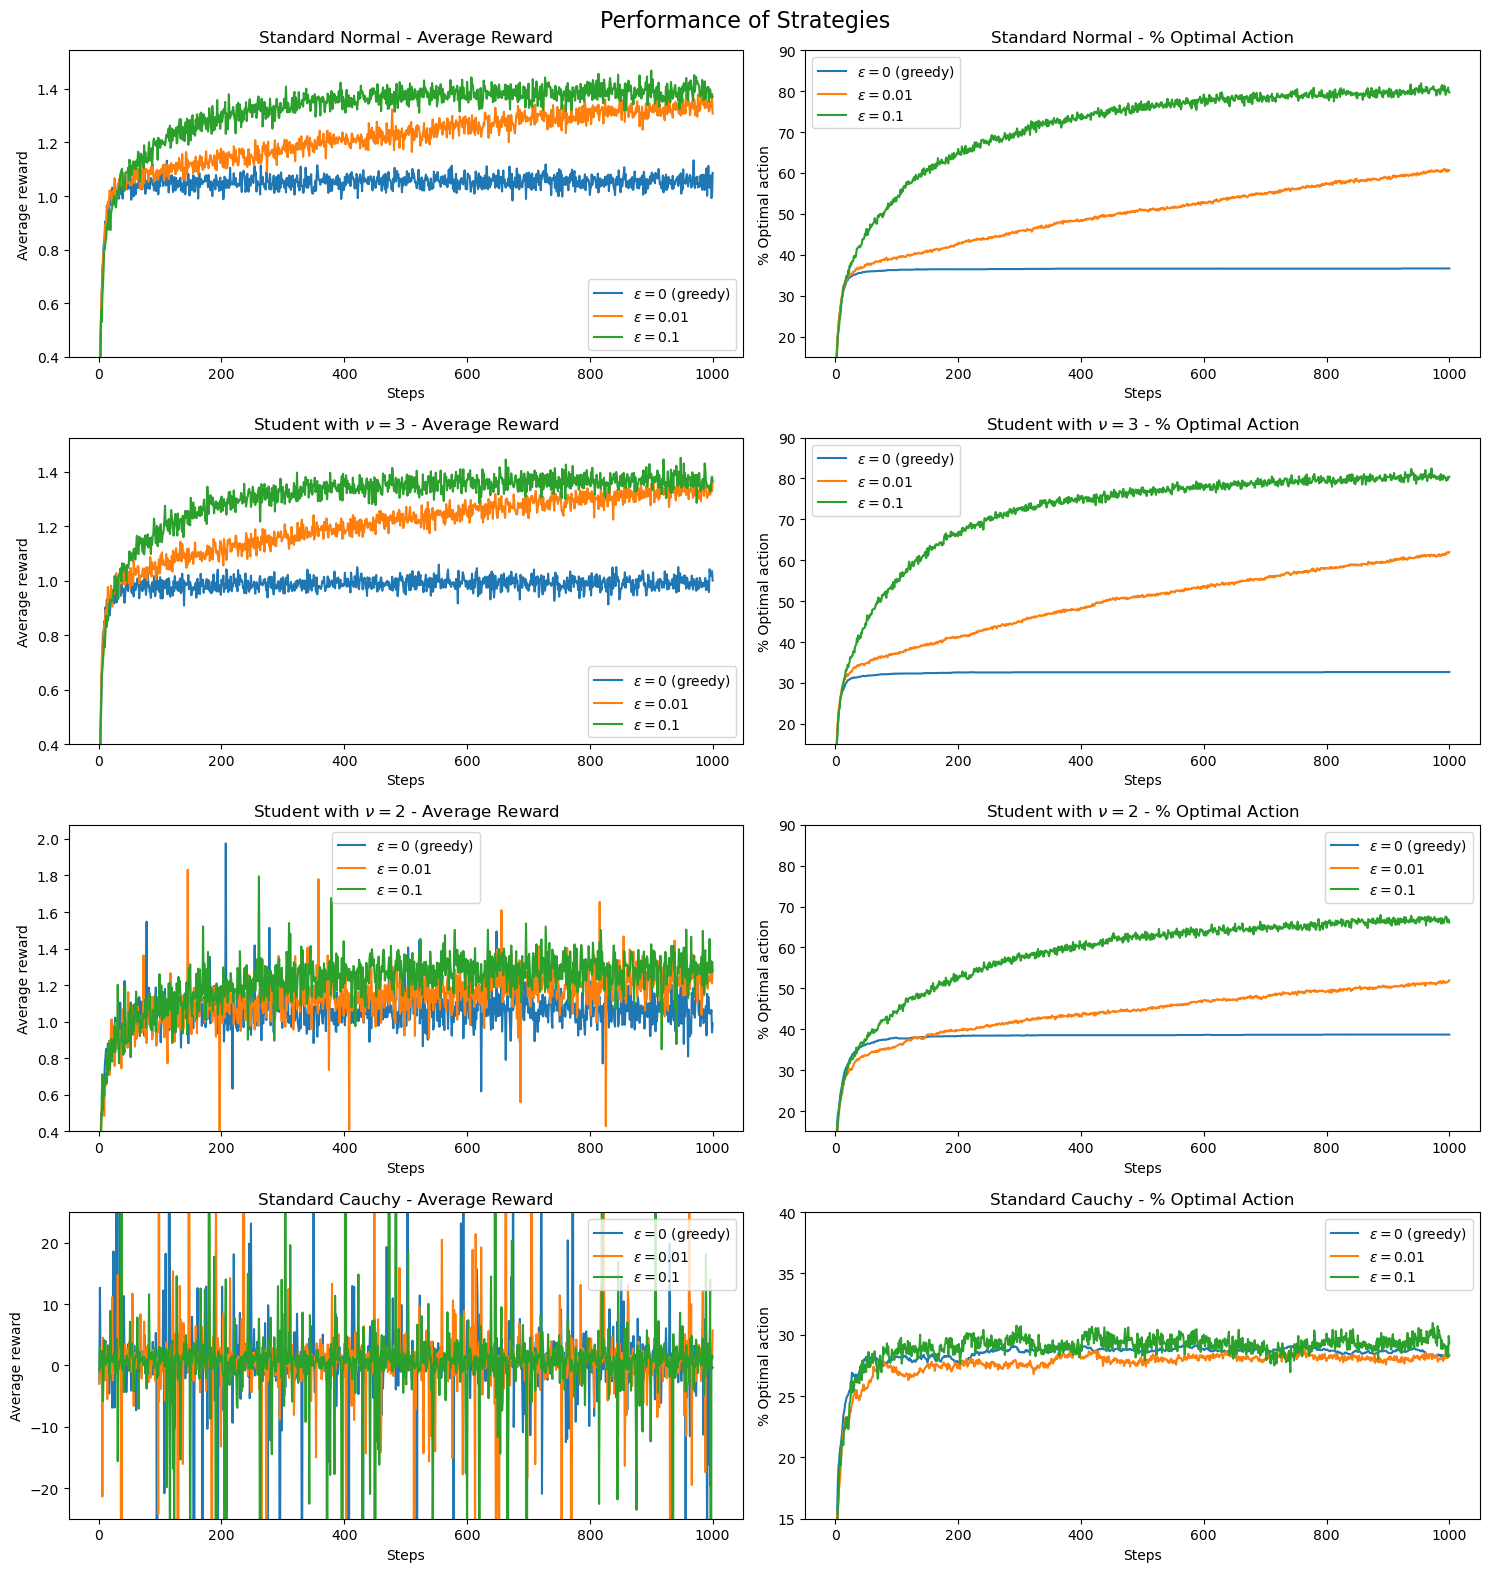
\includegraphics[scale=0.13,center]{images/bandit_tester/eps_greedy_1.png}
    \end{frame}
    \begin{frame}{Результаты -- $\epsilon$-greedy}
        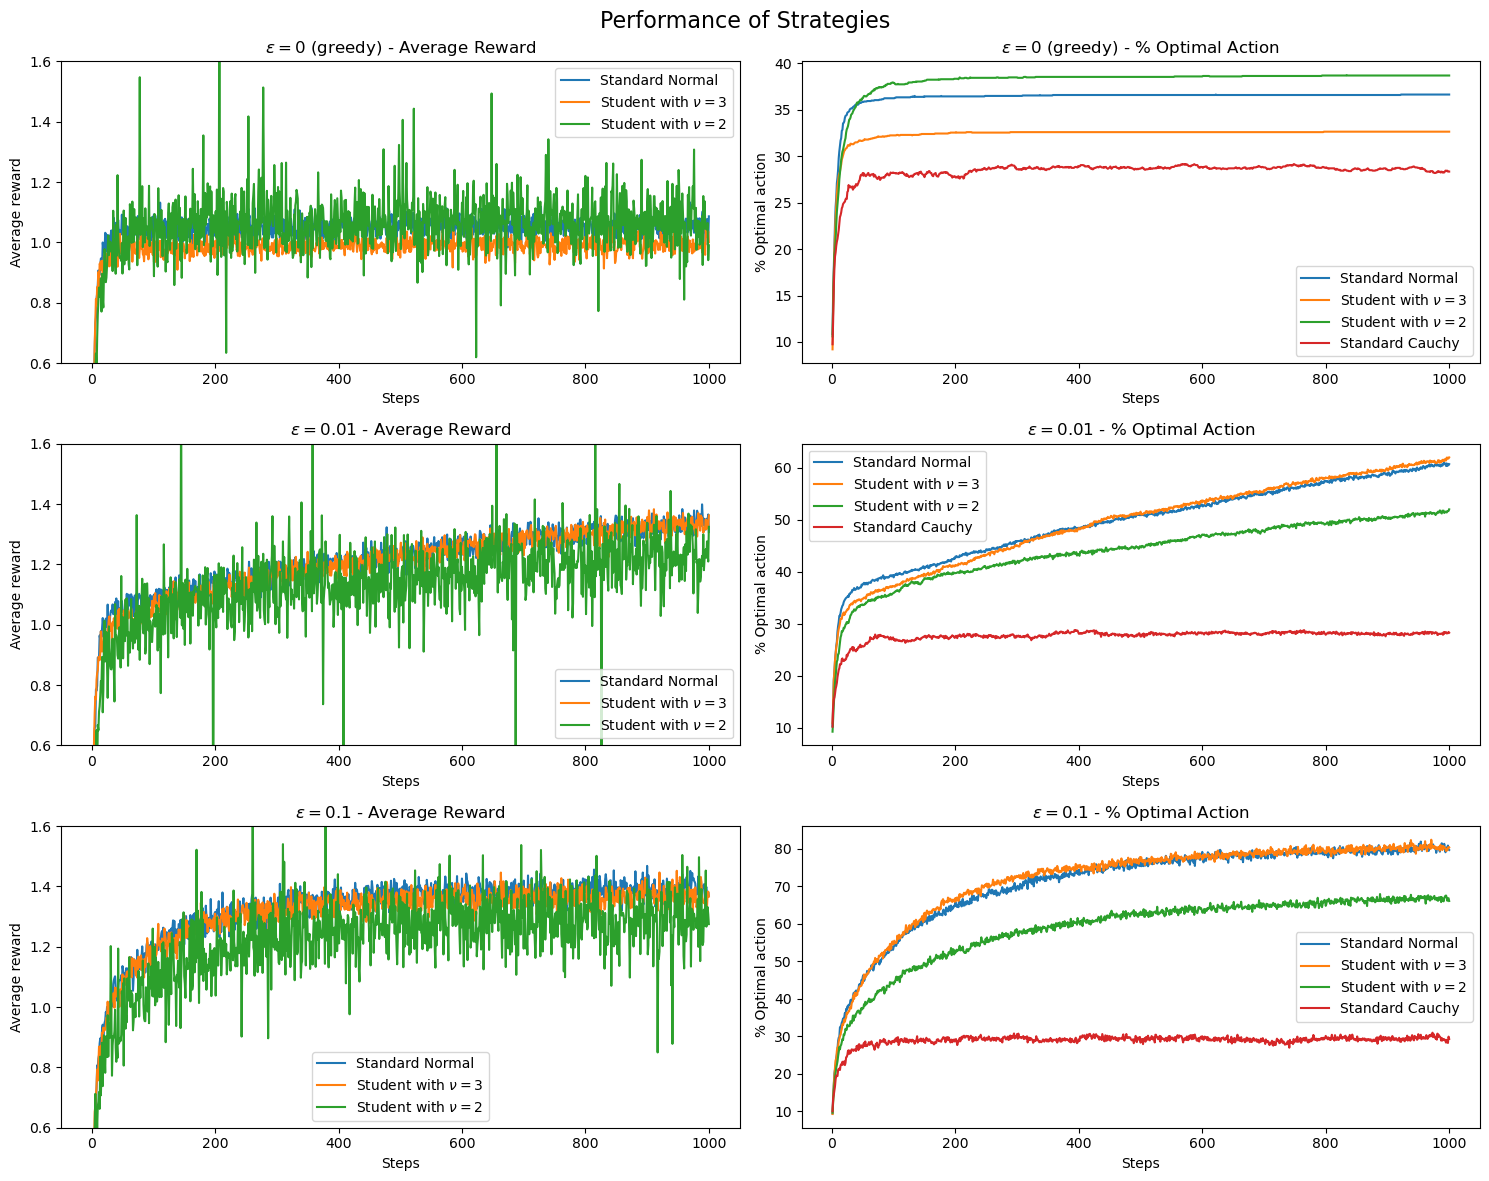
\includegraphics[scale=0.13,center]{images/bandit_tester/eps_greedy_2.png}
    \end{frame}
    \begin{frame}{Результаты -- optimistic initialization}
        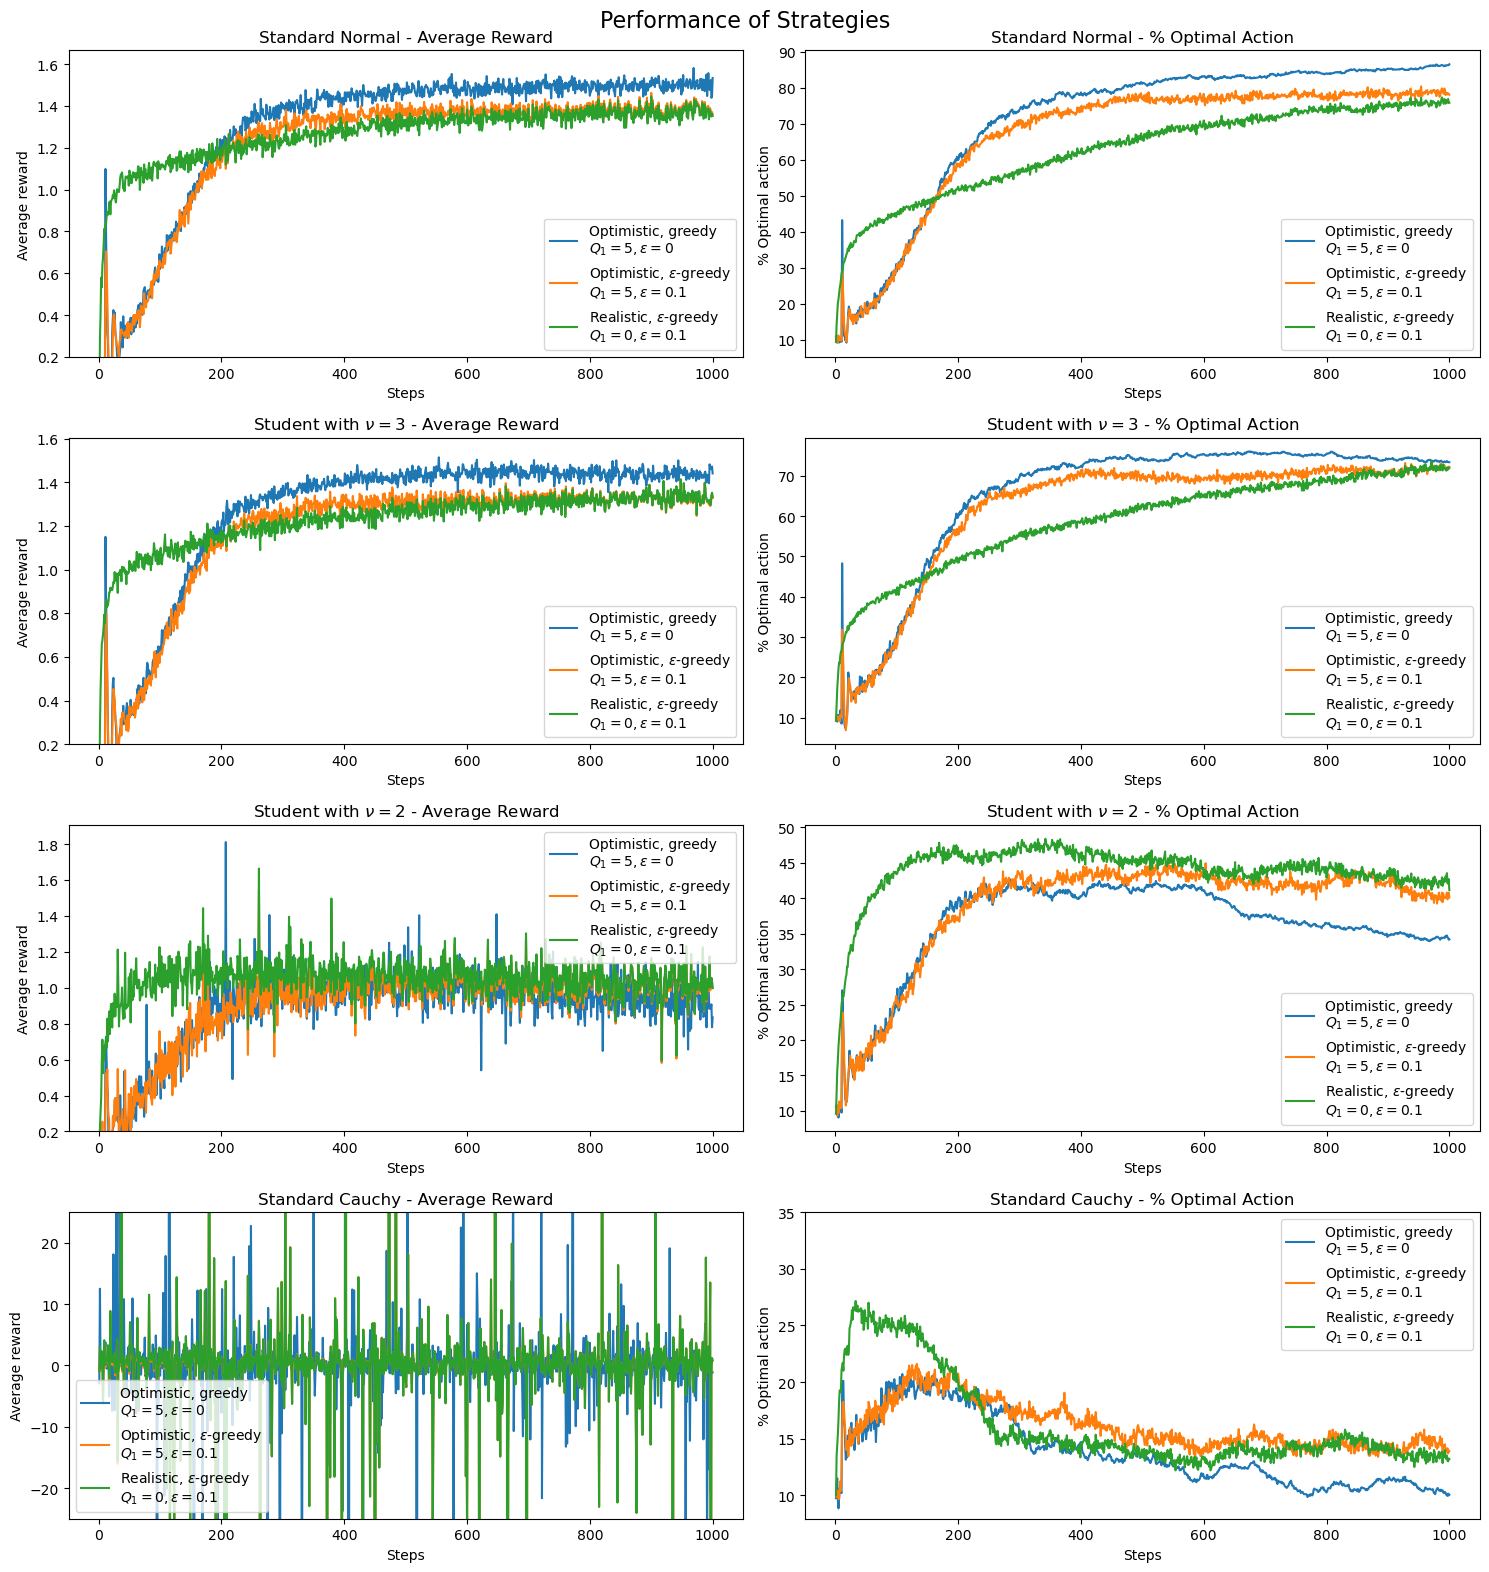
\includegraphics[scale=0.13,center]{images/bandit_tester/optimistic_1.png}
    \end{frame}
    \begin{frame}{Результаты -- optimistic initialization}
        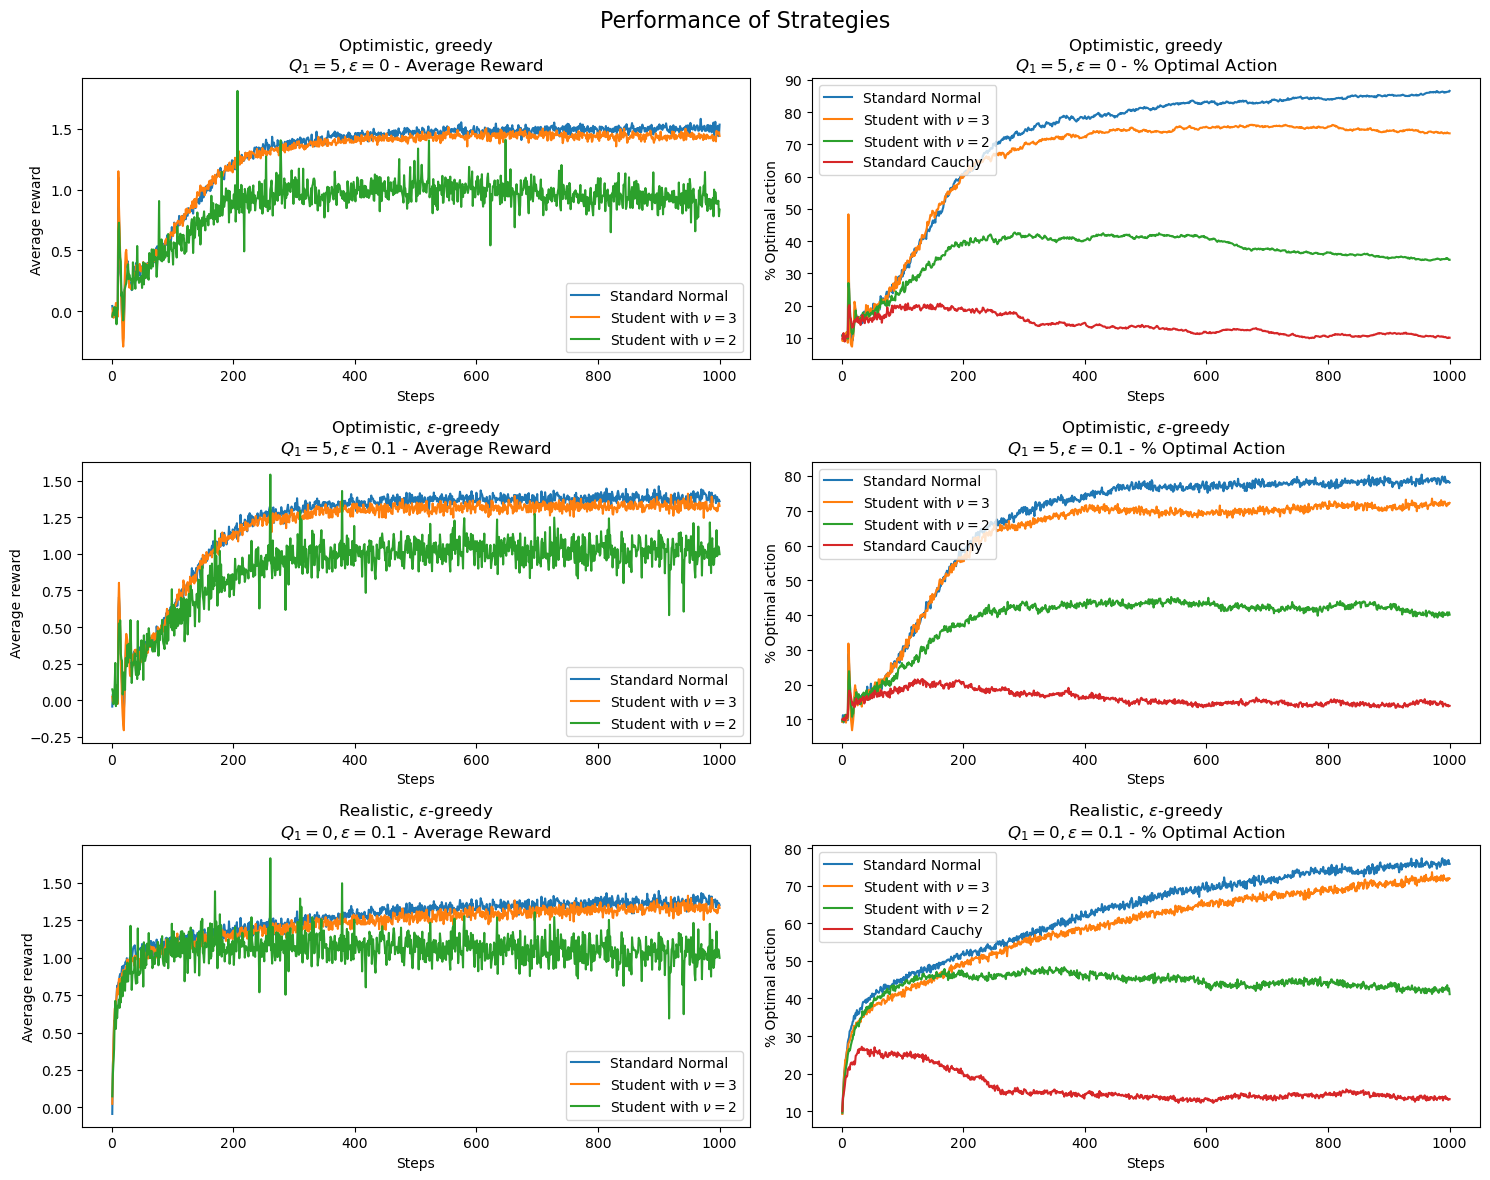
\includegraphics[scale=0.13,center]{images/bandit_tester/optimistic_2.png}
    \end{frame}
    \begin{frame}{Результаты -- UCB}
        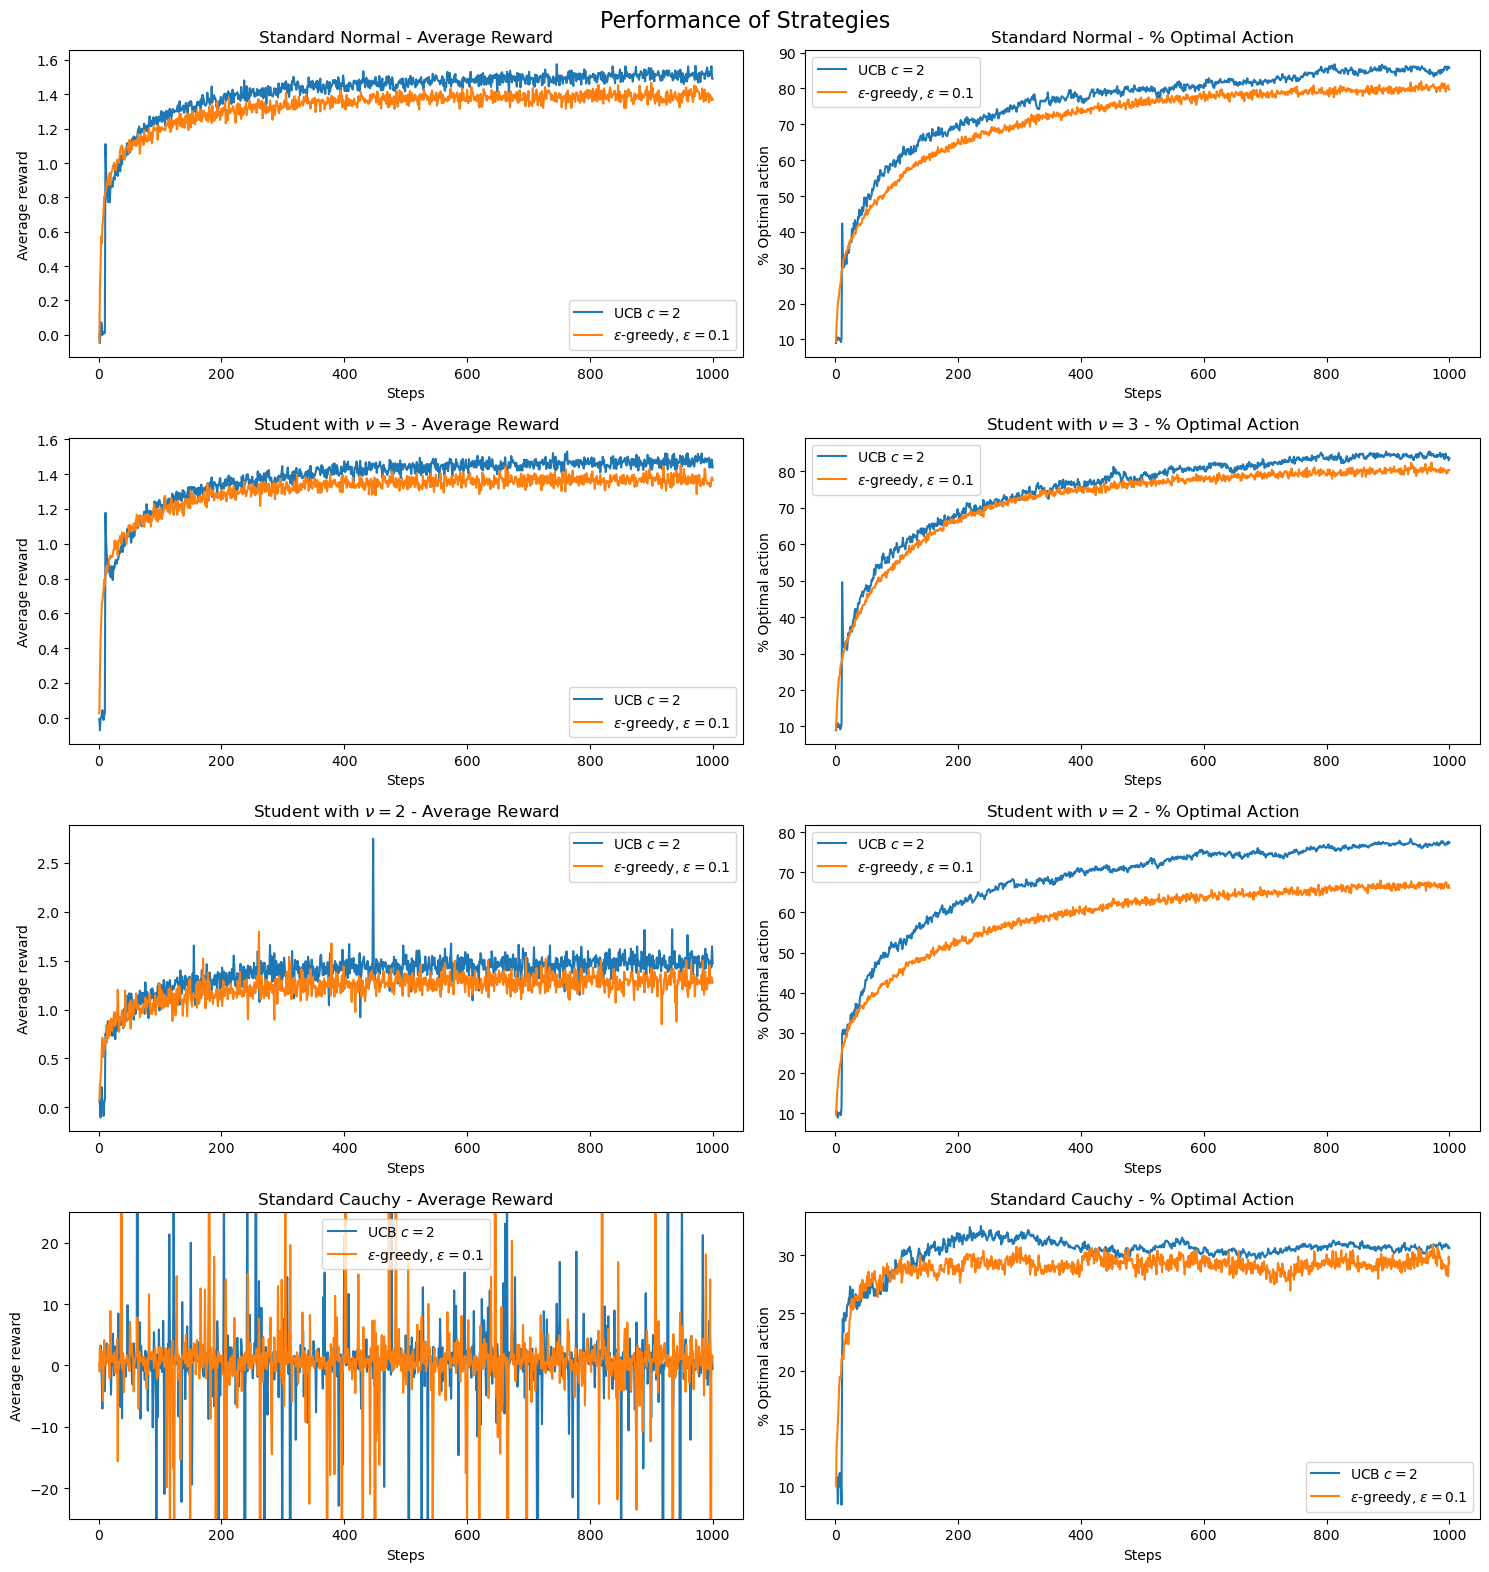
\includegraphics[scale=0.13,center]{images/bandit_tester/ucb_1.png}
    \end{frame}
    \begin{frame}{Результаты -- UCB}
        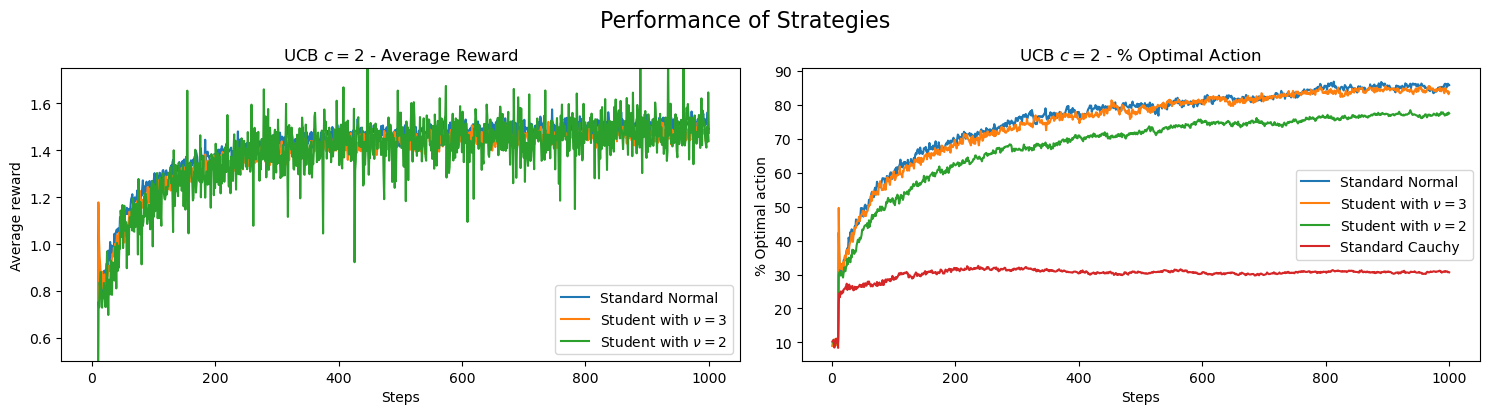
\includegraphics[scale=0.13,center]{images/bandit_tester/ucb_2.png}
    \end{frame}
    \begin{frame}{Результаты -- gradient bandits}
        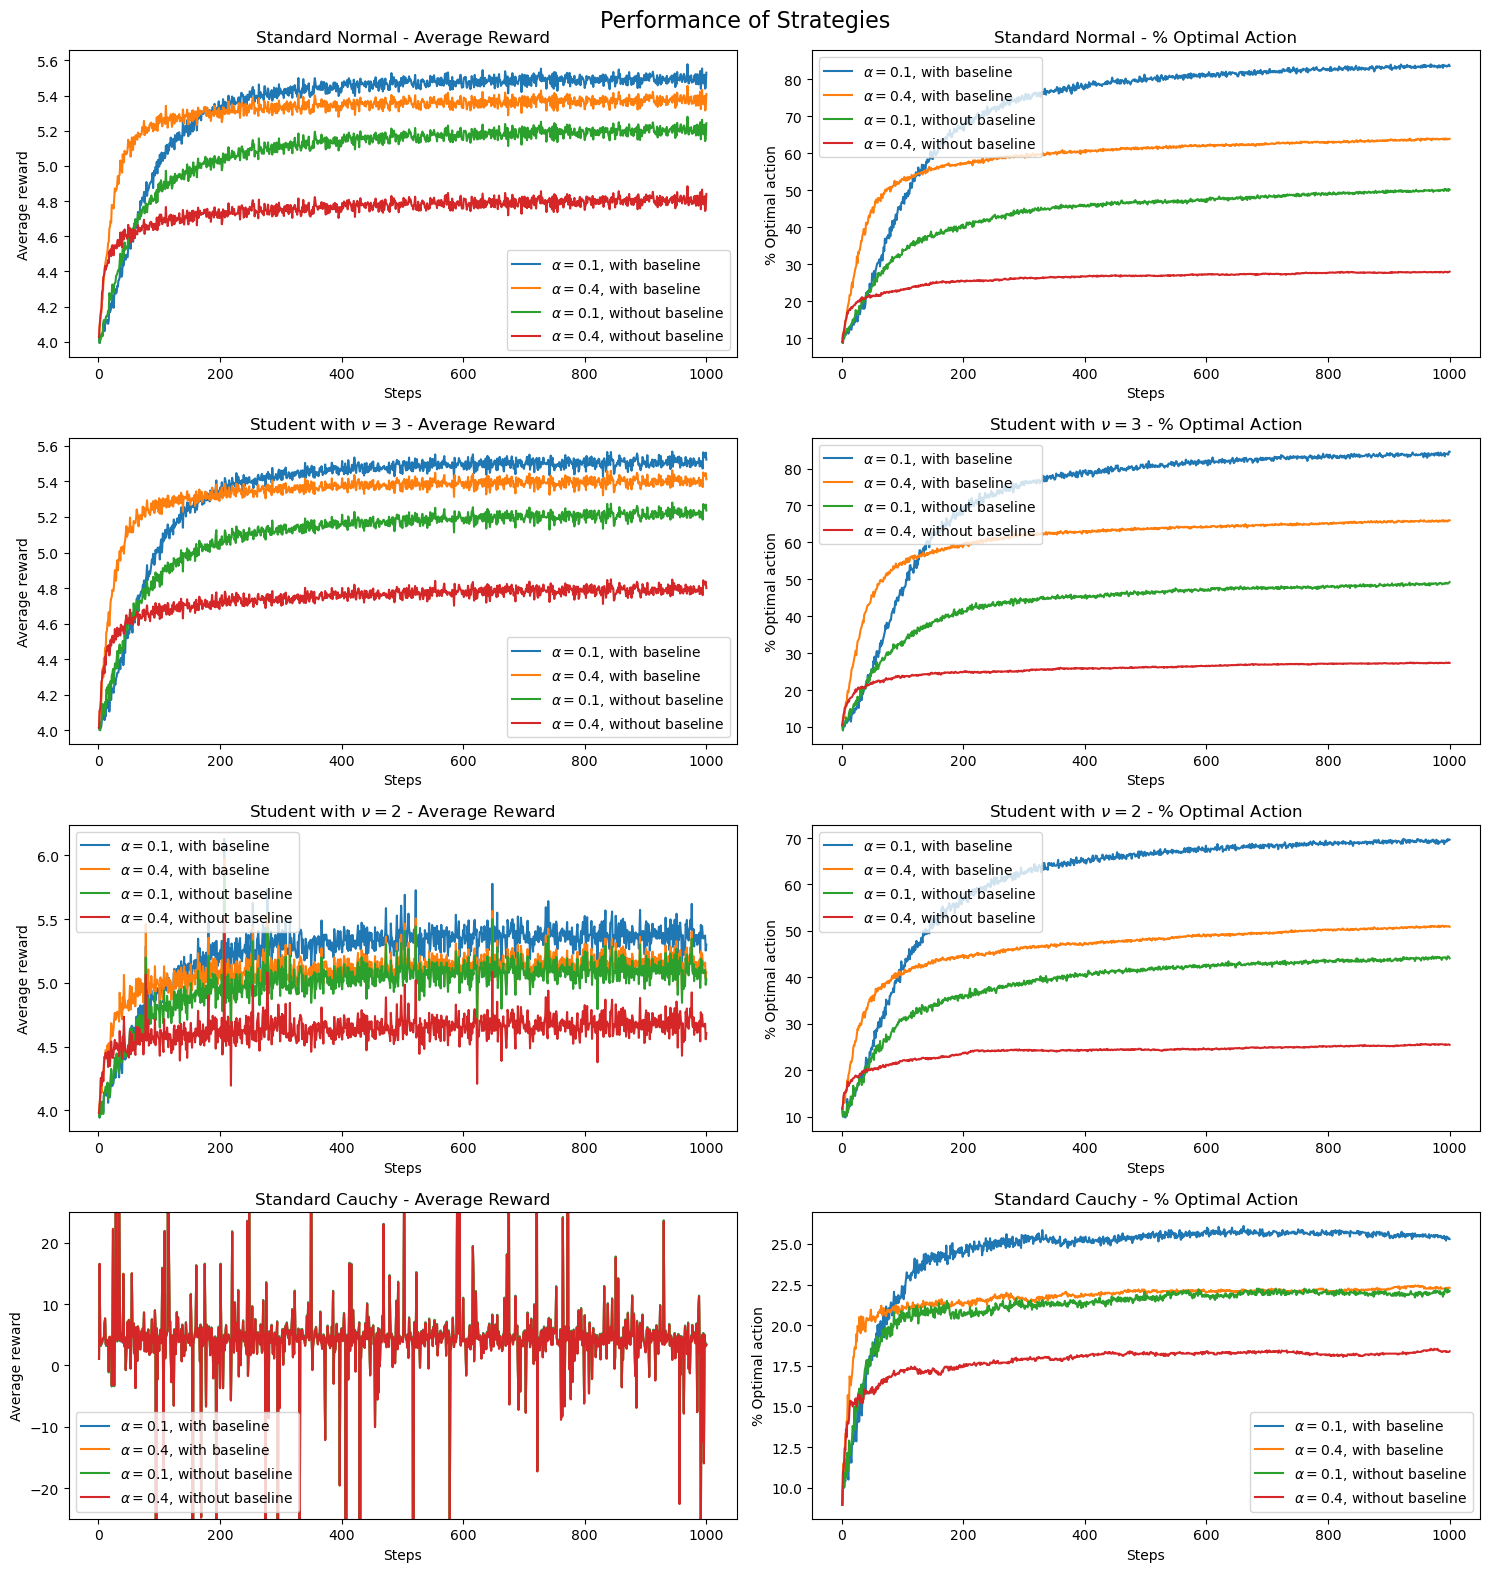
\includegraphics[scale=0.13,center]{images/bandit_tester/gradient_1.png}
    \end{frame}
    \begin{frame}{Результаты -- gradient bandits}
        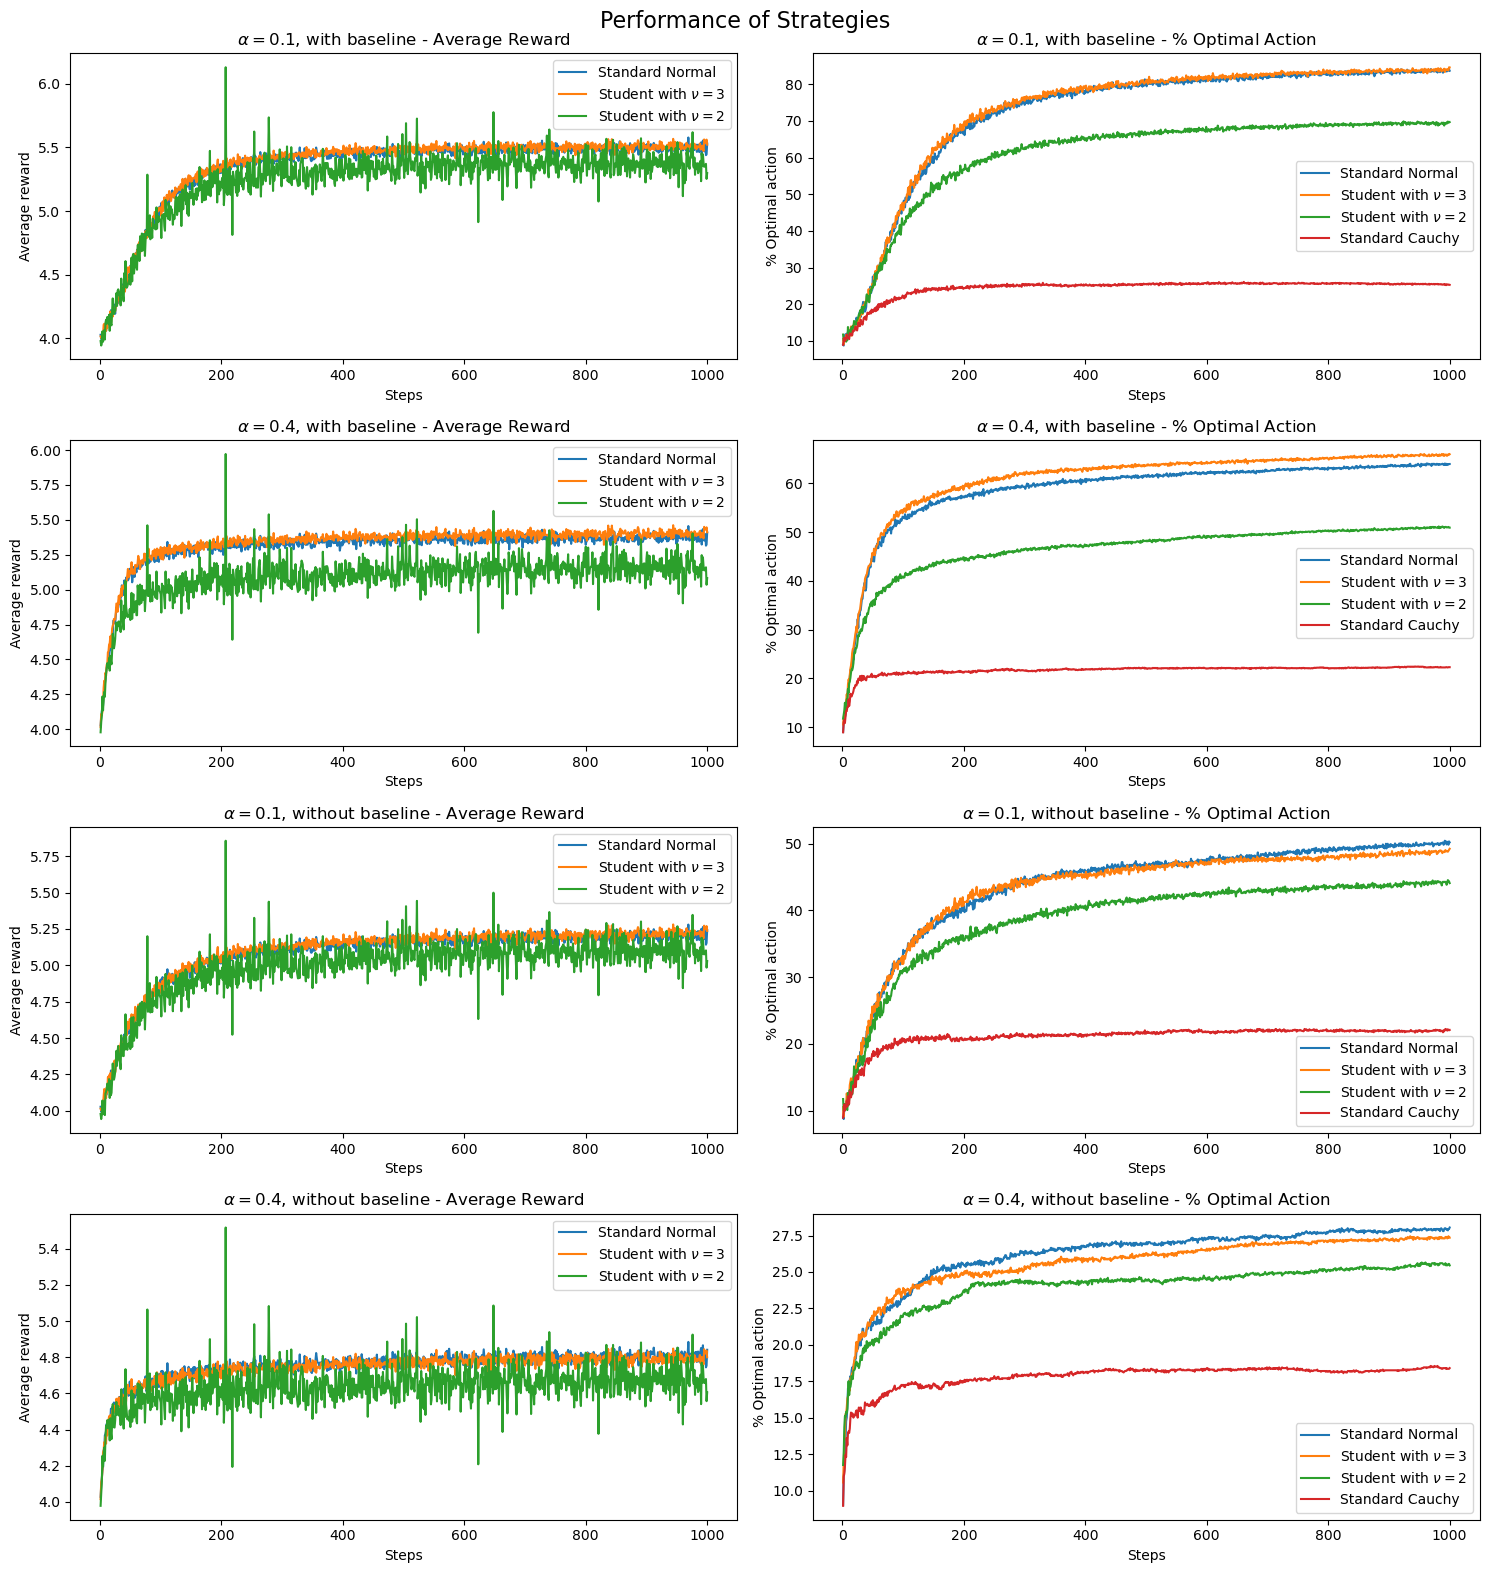
\includegraphics[scale=0.13,center]{images/bandit_tester/gradient_2.png}
    \end{frame}
    \begin{frame}{Результаты -- gradient bandits}
        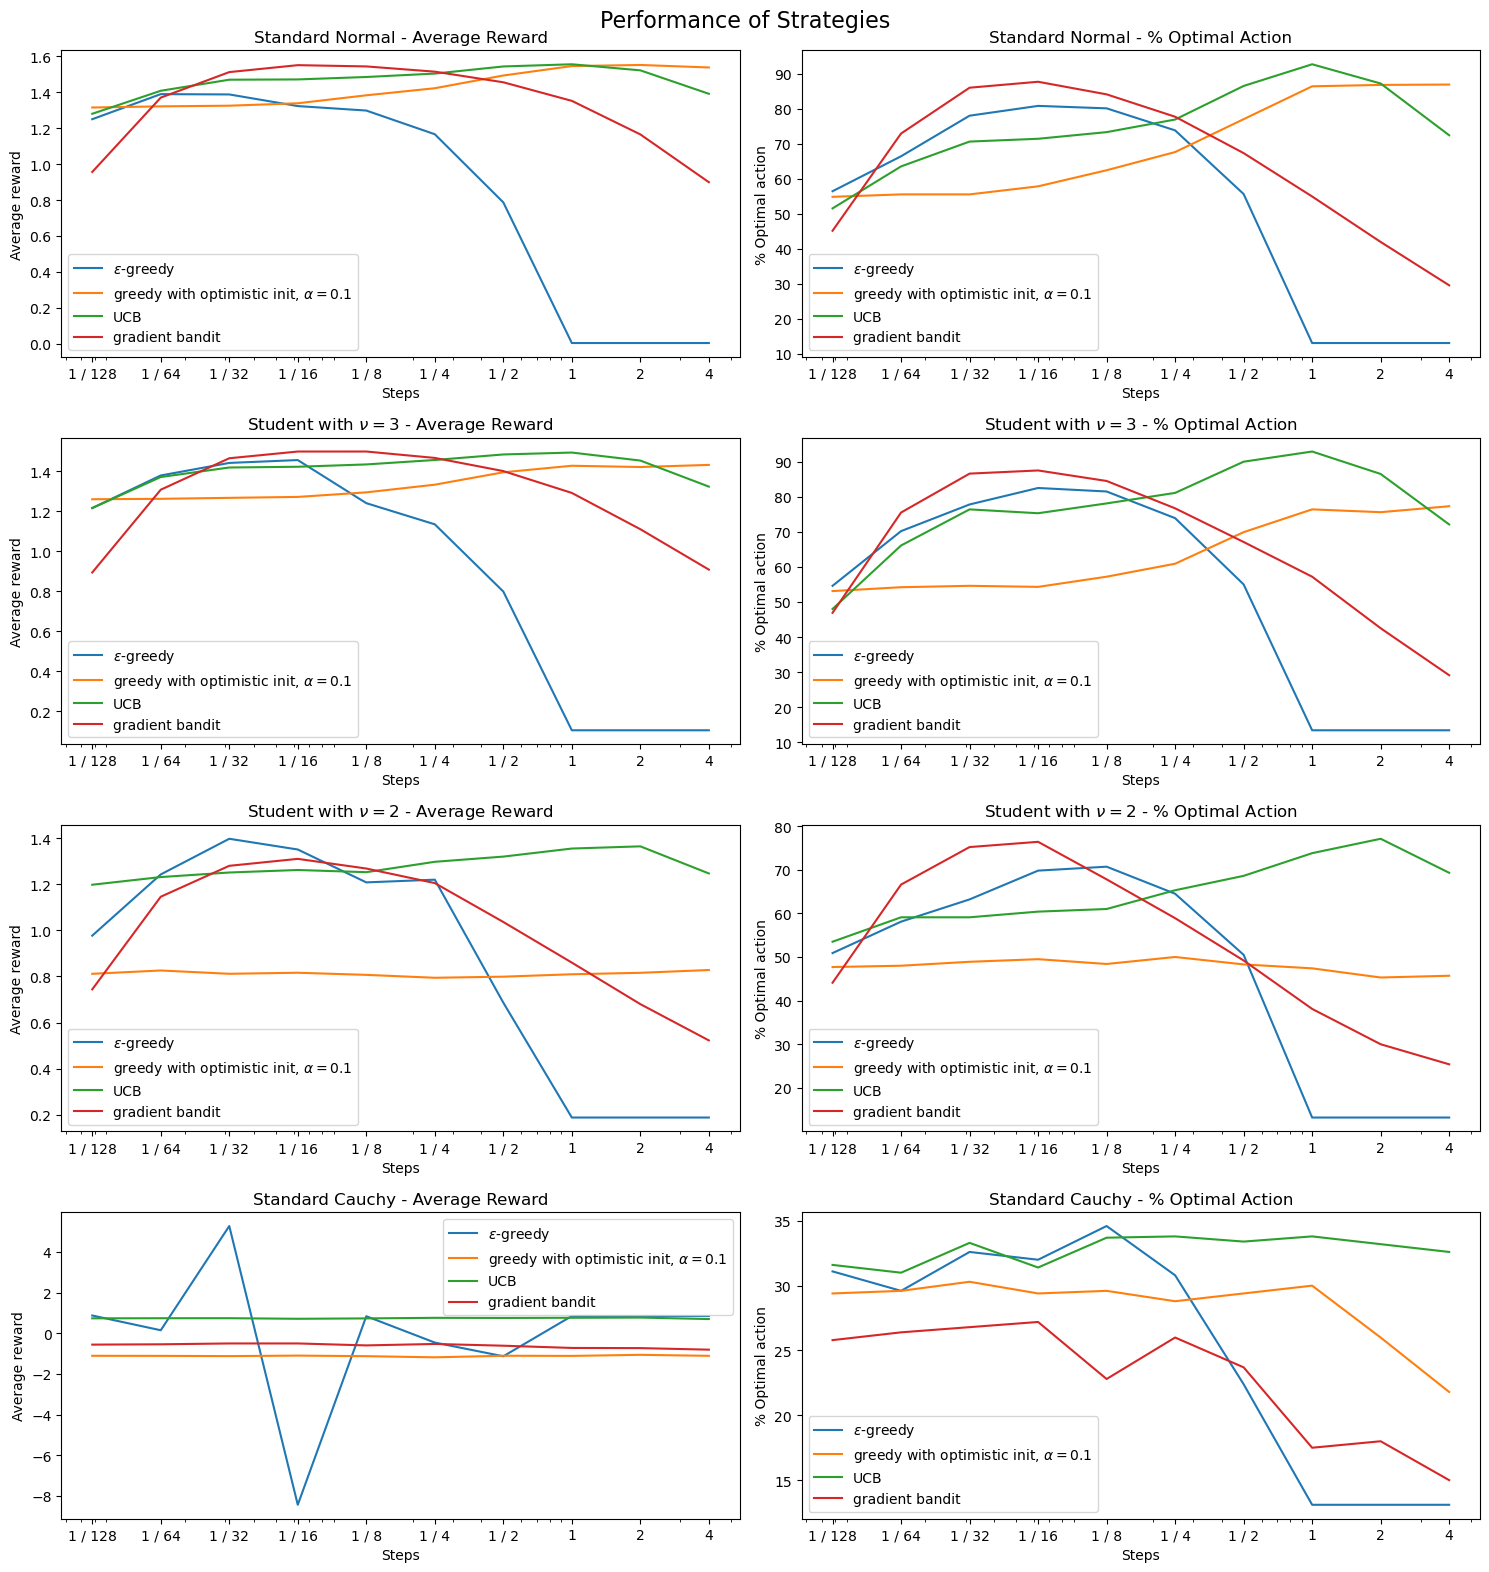
\includegraphics[scale=0.13,center]{images/bandit_tester/overall.png}
    \end{frame}
    \begin{frame}{Выводы}
        Проделанные эксперименты позволяют судить о том, что Gradient bandits, $\epsilon$-greedy и UCB -- стратегии показывают высокую эффективность на степенных распределениях. Так как UCB -- единственная из стратегий, показывающая высокую эффективность на всех метриках и всех распределений, то эта стратегия -- лучший из кандидатов для применения в оптимизации портфолио в модели прироста стоимости акций как многоруких бандитов.
    \end{frame}


\section{Теория}
    \begin{frame}{Неудачные алгоритмы}{слайд 1}
        В каждой из стратегий найдена формула для вычисления оптимальных действий и получен алгоритм, реализующий стратегию.
        \begin{enumerate}
            \item<1-> Каждый ход увеличиваем одну из вероятностей $p_i$ на $\Delta p \geq 0$, а другую вероятность $p_j$ -- уменьшать на $\Delta p$ так, чтобы $V = \textbf{p}^T \cdot \textbf{m} - \lambda (\textbf{p}^2)^T \boldsymbol{\sigma}^2 $ увеличилось на максимально возможное значение.
            \onslide<2->{Проблемы:
            \begin{enumerate}
                \item Каждый ход изменяем только 2 вероятности, поэтому может долго сходиться к оптимальному значению
                \item Долгое время работы одного шага -- $O(n^2)$
                \item Нет гарантий, что сойдется к оптимальному вектору вероятностей
            \end{enumerate}
            }
            \setcounter{currentenumi}{\theenumi}
        \end{enumerate}
    \end{frame}
    \begin{frame}{Неудачные алгоритмы}{слайд 2}
        \begin{enumerate}
        \setcounter{enumi}{\thecurrentenumi}
            \item<1-> Каждый ход увеличиваем одну из вероятностей $p_i$ на $\Delta p_{\uparrow}$, а все остальные ненулевые вероятности -- уменьшать на $\frac{\Delta p_{\uparrow}}{\phi_{t,i}}$, где $\phi_{t,i} := \phi_t - I_{p_i \neq 0}$.
            \onslide<2->{Проблемы:
                \begin{enumerate}
                    \item Долгое время работы одного шага -- $O(n^2)$
                    \item Нет гарантий, что сойдется к оптимальному вектору вероятностей
                \end{enumerate}
            }
        \end{enumerate}
    \end{frame}
    \begin{frame}{Первый рабочий алгоритм}
        \begin{block}{Замечание 1}
            $V$ вогнута на $R^n$
        \end{block}
        \begin{block}{Замечание 2}
            $\Delta^n$ замкнуто и выпукло в $R^n$
        \end{block}
        \onslide<2->{Тогда можно найти оптимальный вектор вероятностей с помощью метода градиентного подъема. В качестве алгоритма был взят метод за $O(1)$, описанный в статье \cite{cauchy_simplex}}
        \onslide<3->{Проблема: получаемый вектор может иметь небольшую погрешность}
    \end{frame}
    \begin{frame}{Второй рабочий алгоритм}
        \onslide<1->{
        \begin{alertblock}{Утверждение 1}
            Пусть $w_i = \frac{\partial V}{\partial p_i} = m_i - 2\lambda p_i \sigma_i^2$. Тогда $P \in \Delta^n$ является решением уравнения $\textbf{p} = \underset{\textbf{p} \in \Delta^n}{\arg \max} \: \left(\textbf{p}^T \cdot \textbf{m} - \lambda \left(\textbf{p}^T\right)^2 \cdot \boldsymbol{\sigma}^2 \right)$ тогда и только тогда, когда $\forall \, i,j: \: i \neq j \: \land p_i \neq 0 \: \land p_j \neq 0 \hookrightarrow w_i(p_i) = w_j(p_j) = w$ и $\forall \, i,j: \: p_i = 0, p_j \neq 0 \hookrightarrow w_i(p_i) \leq w_j(p_j)$
        \end{alertblock}
        }
        \onslide<2->{
        \begin{alertblock}{Утверждение 2}
            Если упорядочить все $m_i$ по возрастанию и сопоставить каждому $m_i$ свой $p_i$ из оптимального вектора вероятностей, то все нулевые вероятности будут находиться ``не правее'' ненулевых вероятностей, причем в какой-то точке могут находиться одновременно ненулевые и нулевые вероятности только в том случае, когда неулевым вероятностям соответствуют безрисковые рычаги.
        \end{alertblock}
        }
    \end{frame}
    \begin{frame}{Второй рабочий алгоритм}
        \begin{block}{Утв. 3 (из портфельной теории Марковица)}
            Если $\forall i \sigma_i^2 > 0$ и $\exists i,\, j: \: m_i \neq m_j$, то существует метод нахождения $\textbf{p} = \underset{\textbf{p} \in R^n}{\arg \max} V(\textbf{p})$ на гиперплоскости $p_1 + ... + p_n = 1$, и для $\textbf{p}$ в таком случае верно, что 
            $$p_i = \frac{m_i}{2\lambda \sigma_i^2} + \frac{1 - \Sigma_1}{\Sigma_0} \cdot \frac{1}{2 \lambda \sigma_i^2}$$
            где 
            $$\Sigma_0 = \sum_{i=1}^n \frac{1}{2 \lambda \sigma_i^2}, \; \Sigma_1 = \sum_{i=1}^n \frac{m_i}{2 \lambda \sigma_i^2}$$
        \end{block}
    \end{frame}
    \begin{frame}{Второй рабочий алгоритм}
        \begin{block}{Утв. 4 (из портфельной теории Марковица)}
            Если $\exists! \, i: \: \sigma_i^2 = 0$, то есть существует безрисковый рычаг (пусть его среднее $m_0$), то существует метод нахождения $\textbf{p} = \underset{\textbf{p} \in R^n}{\arg \max} V(\textbf{p})$ на гиперплоскости $p_1 + ... + p_n = 1$, и $p_i = \frac{m_i - m_0}{2 \lambda \sigma_i^2} \cdot \left(1 + m_0 \frac{\Sigma_1'}{\Sigma_2'} \right)$, где $\Sigma_k' = \sum_{i=1}^n \frac{(m_i - m_0)^k}{2 \sigma_i^2}$ и $i \neq 0$.
        \end{block}
    \end{frame}
    \begin{frame}{Второй рабочий алгоритм}
        Пусть мы отсортировали все рычаги и отбросили все, что хуже наилучшего безрискового. Достаточно найти такое $t$, что $\forall i$ либо $m_i \leq t \land p_i = 0$, либо $m_i > t \land w_i = t \Leftrightarrow p_i = \frac{m_i - t}{2\lambda \sigma_i^2}$ и $\sum_{i=1}^n p_i = \sum_{i=1}^n p_i(t) = 1$. \pause \\ Для каждого $t$ однозначно определен набор тех $i$, для которых вероятности ненулевые, а именно такие $i$, что $m_i > t$. Кроме того, заметим, что при уменьшении $t$ сумма вероятностей увеличивается, а при $t = m_{(j)}$ (то есть $j$-ая порядковая статистика) верно, что 
        $$\sum_{i=1}^n p_i(m_{(j)}) = \sum_{i=j+1}^n \frac{m_{(i)} - m_{(j)}}{2 \lambda \sigma_{(i)}^2} = \sum_{i=j+1}^n \frac{m_{(i)}}{2 \lambda \sigma_{(i)}^2} \: - m_{(j)} \sum_{i=j+1}^n \frac{1}{2 \lambda \sigma_{(i)}^2} $$
    \end{frame}
    \begin{frame}{Второй рабочий алгоритм}
        Если обозначить $\sum_{i=j+1}^n \frac{m_{(i)}}{2 \lambda \sigma_{(i)}^2} := \Sigma_1(j+1)$, а $\sum_{i=j+1}^n \frac{1}{2 \lambda \sigma_{(i)}^2} := \Sigma_0(j+1)$, то 
        $$
            \sum_{i=1}^n p_i(m_{(j)}) = \Sigma_1(j+1) - m_{(j)} \Sigma_0(j+1)
        $$
        причем $\Sigma_1(n+1) = \Sigma_0(n+1) = 0$ и $$\Sigma_1(i) = \Sigma_1(i+1) + \frac{m_{(i)}}{2\lambda \sigma_{(i)}^2}, \: \Sigma_0(i) = \Sigma_0(i+1) + \frac{1}{2\lambda \sigma_{(i)}^2}$$
    \end{frame}
    \begin{frame}{Второй рабочий алгоритм}
        Ввиду увеличения суммы вероятностей оптимальное $t$ либо лежит на полуинтервале \\ $(m_{(i)}, m_{(i+1)}]$ и $\sum_{j=1}^n p_j (m_{(i+1)}) \leq 1 < \sum_{j=1}^n p_j (m_{(i)})$, либо лежит на луче $(-\infty, m_{(1)})$ и $\sum_{j=1}^n p_j (m_{i+1}) \leq 1$. Во всех случаях мы можем вычислить $p_i$ по формулам из пункта, учитывая только те $i$, для которых $m_{(i)} \geq t$, то есть все $m_{(i)}$ от конца интервала, где находится $t$, и до $m_{(n)}$.
    \end{frame}
    \begin{frame}{Описание алгоритма}
        \begin{enumerate}
            \item<1-> Сортируем все $m_i$ по убыванию, в случае равенства по возрастанию $\sigma_i^2$. Работает за $O(n \log n)$.
            \item<2-> С начала массива ищем безрисковый рычаг с наибольшим матожиданием. Если нашли (это первый рычаг с $\sigma_i^2 = 0$), то отбрасываем все рычаги правее найденного $\left(O(n) \right)$. 
            \item<3-> Если отбросили все рычаги, кроме безрисокового, то вероятность выбора безрискового рычага равна 1, заканчиваем работу $\left( O(1) \right)$.
            \item<4-> Иначе считаем $\Sigma_1(n+1) = \Sigma_0(n+1) = 0$, проходимся слева направо по $m_{(i)}$, пересчитывая за $O(1)$ $\Sigma_1(i+1)$ и $\Sigma_0(i+1)$, вычисляя за $O(1)$ сумму вероятностей. Находим первое такое $i$, что $\sum_{i=1}^n p_i(m_{(i+1)}) \leq 1$ и $\sum_{i=1}^n p_i(m_{(i+1)}) > 1$ $\left( O(n) \right)$.
            \item<5-> Если такое $i$ нашлось, то $p_j$ для $j \geq i + 1$ вычисляются по формулам из пункта  а для $j \leq i \hookrightarrow p_j = 0$. Если же не нашлось, то у всех рычагов ненулевые вероятности, и, аналогично, по формулам из пункта  вычисляются все $p_i$ $\left( O(n) \right)$.
        \end{enumerate}
    \end{frame}
    \begin{frame}{Особенности алгоритма}
        Плюсы:
        \begin{enumerate}
            \item<1-> Работает за $O(n \log n)$ вместо $O(n^2)$, причем этот $n \log n$ ``лёгкий'', поскольку в него включена лишь сортировка.
            \item<2-> Дает точное решение
        \end{enumerate}
        \onslide<3->{
        Минусы:
        \begin{enumerate}
            \item Проблема холодного старта
        \end{enumerate}
        }
    \end{frame}
    \begin{frame}{Модификации исходных алгоритмов}
        \begin{enumerate}
            \item<1-> $\epsilon$-greedy стратегии:
            \begin{itemize}
                \item Классический
                \item Adaptive: на $t$-ом шаге $\epsilon_t = \frac{1}{t}$ 
                \item VDBE: 
                $
                \epsilon_{t+1} = \delta  \frac{\left| e^{w_t(a)/\tau} - e^{w_{t+1}(a)/\tau} \right|}{e^{w_t(a)/\tau} + e^{w_{t+1}(a)/\tau}}  + (1 - \delta) \epsilon_t
                $, где $w_t(a) = \frac{\partial V}{\partial p_a}$ на $t$-ом шаге, $\tau$ -- температура
            \end{itemize}
            \item<2-> Positive initialization: инициализируем $Q_0(a) = q > 0, \; Q^2_0(a) = q^2$.
            \item<3-> Аналог UCB: В алгоритме за $O(n \log n)$ считаем, что $m_i = q_i + c \sqrt{\frac{\ln T}{N_t(a)}}$
            \item<4-> Аналог gradient bandits
        \end{enumerate}
    \end{frame}
    


\section{Итоговые эксперименты}
    \begin{frame}{Параметры}
        \begin{itemize}
            \item<1-> Кол-во тестов -- 2000, длина теста -- 1000 шагов
            \item<2-> Распределения рычагов (все рычаги брались из одного семейства распределений):
            \begin{itemize}
                \item Нормальное ($t_{\infty}$)
                \item Распределение Стьюдента с $\nu = 3$ ($t_3$) 
                \item Распределение Стьюдента с $\nu = 2.1$ ($t_{2.1}$)
                \item Распределение Стьюдента с 2 степенями свободы $t_2$
            \end{itemize}
            \item<3-> Матожидание бралось из $N(1,1)$, дисперсия бралась из $Exp(2)$
        \end{itemize}
    \end{frame}
    \begin{frame}{Метрики}
        \begin{itemize}
            \item <1-> Среднее сожаление: если $V_{max} = (\textbf{p}_{max}^T \cdot \textbf{m} - \lambda (\textbf{p}_{max}^2)^T \cdot \boldsymbol{\sigma}^2)$, где $\textbf{p}_{max}$ -- оптимальный вектор вероятностей, то $Reg_t = V_{max} - (\textbf{p}_t^T \cdot \textbf{q} - \lambda (\textbf{p}_{t}^2)^T \cdot \textbf{s}^2)$. Если $Reg_t < 0$, то алгоритм ``переоценивает'' себя.
            \item <2-> Среднее реальное сожаление: $RReg_t = V_{max} - (\textbf{p}_t^T \cdot \textbf{m} - \lambda (\textbf{p}_{t}^2)^T \cdot \boldsymbol{\sigma}^2)$. Всегда $\geq 0$.
            \item <3-> Процент оптимальных действий: $$\delta = 1 - \frac{1}{2}\sum_{i=1}^n |p_i - p_{i, max}|$$
        \end{itemize}
    \end{frame}
    \begin{frame}{Графики}
        Были построены графики, сгруппированные по каждому семейству распределений и по каждому алгоритму. Кроме того, были построены графики для различных значений $\lambda \in [0.1,\, 0.3,\, 0.6,\, 1,\, 2,\, 4]$.
    \end{frame}
    \begin{frame}{Первый рабочий алгоритм}
        Предварительно был реализован первы рабочий алгоритм через градиентный подъем, после чего на примерах были сравнены оба алгоритма. Результаты совпадают в пределах погрешности.
    \end{frame}
    \begin{frame}{Результаты -- $\epsilon$-greedy}
        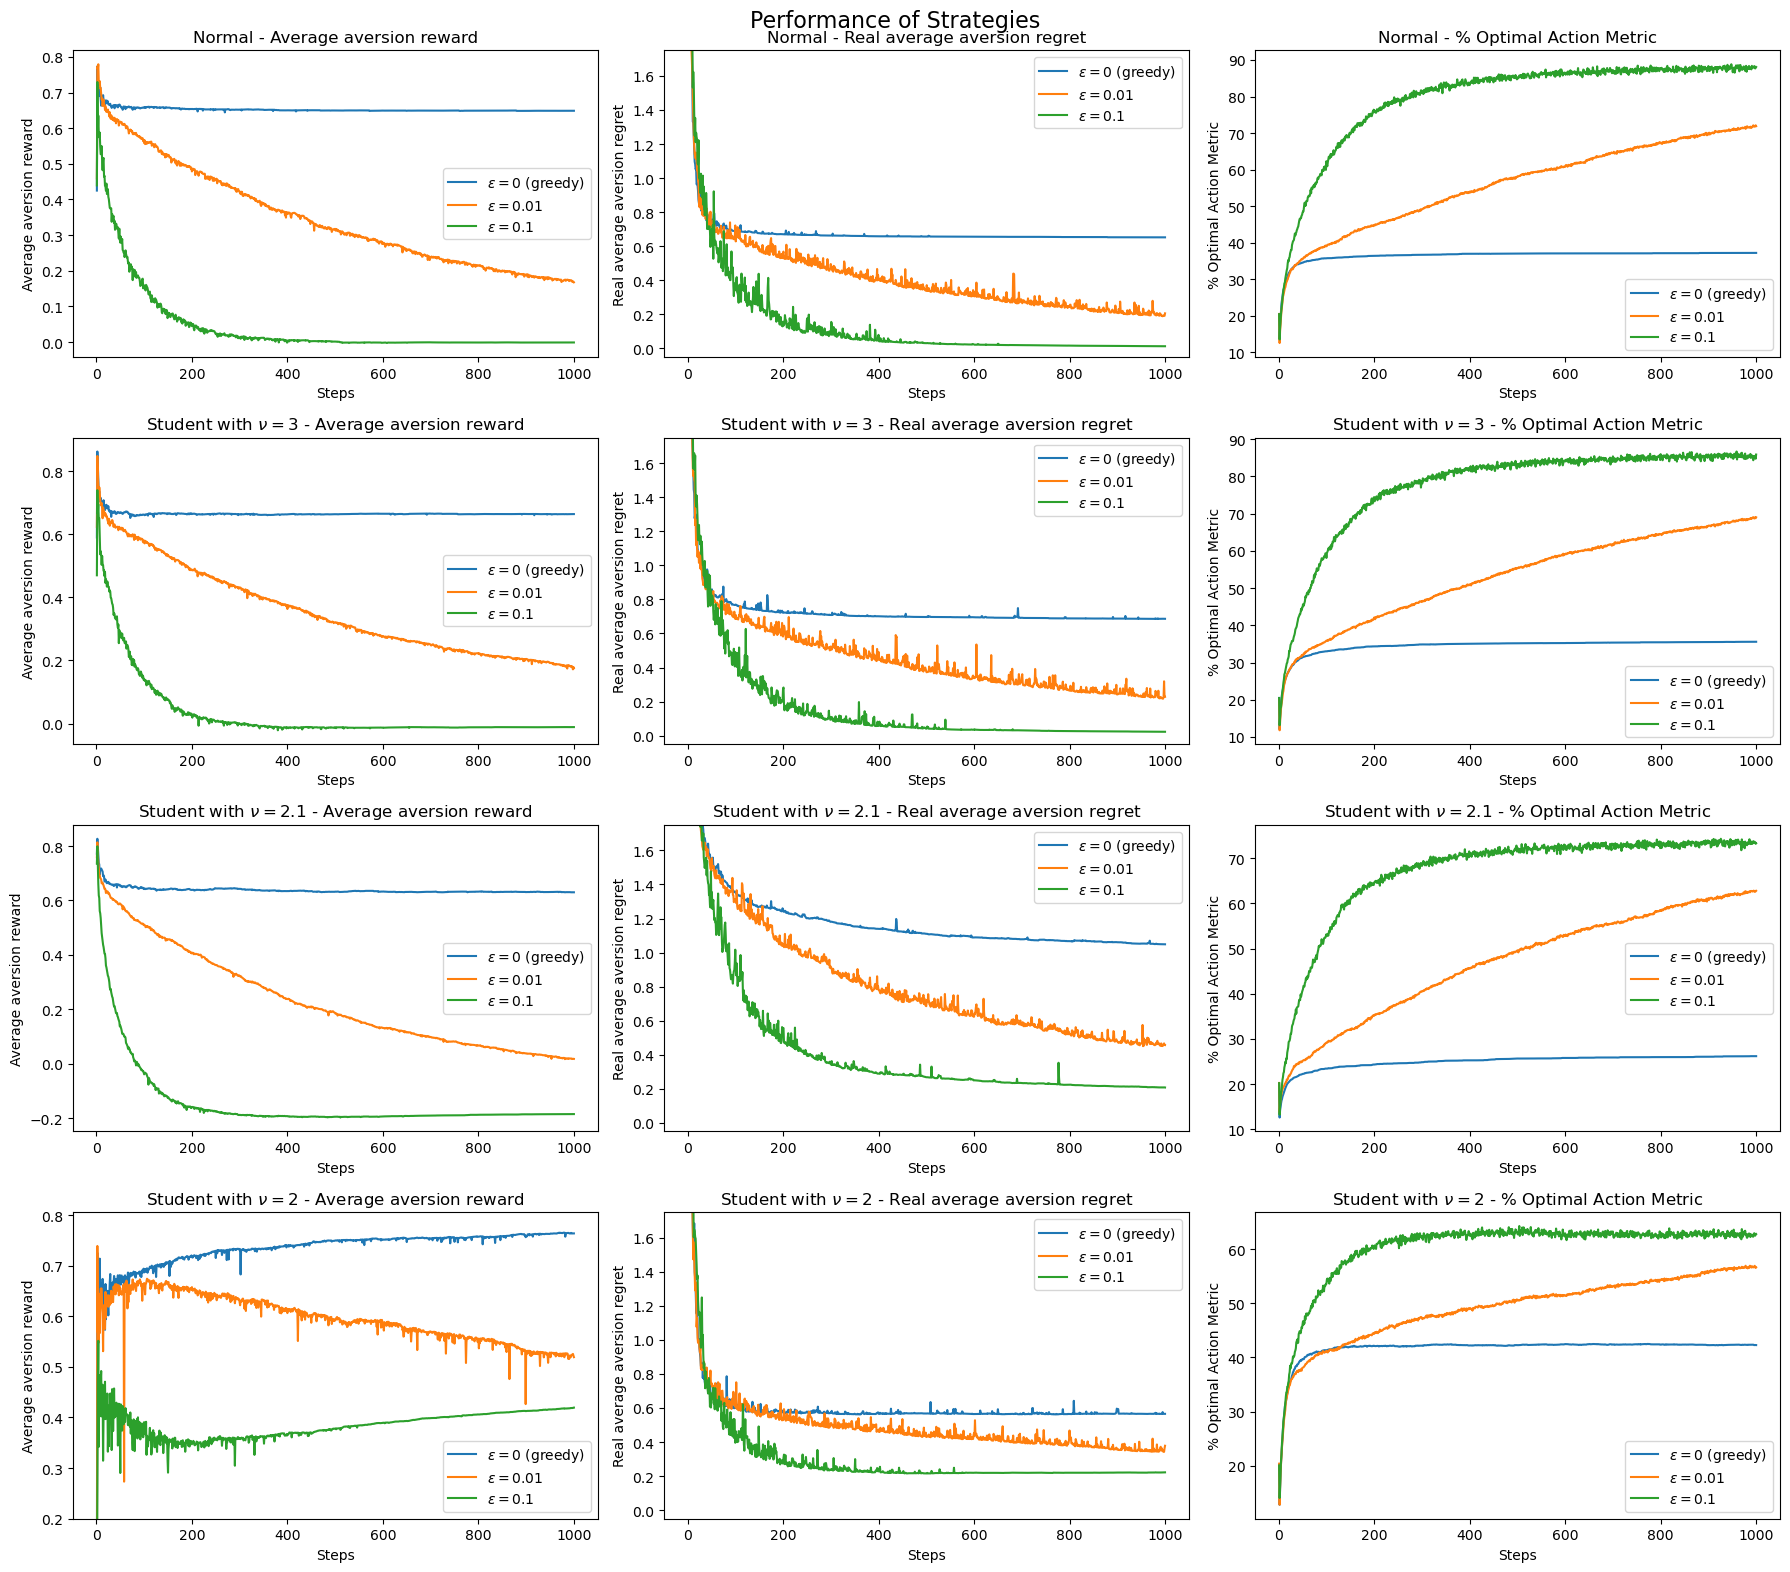
\includegraphics[scale=0.13,center]{images/theory_images/epsilon_greedy/one_distr.png}
    \end{frame}
    \begin{frame}{Результаты -- $\epsilon$-greedy}
        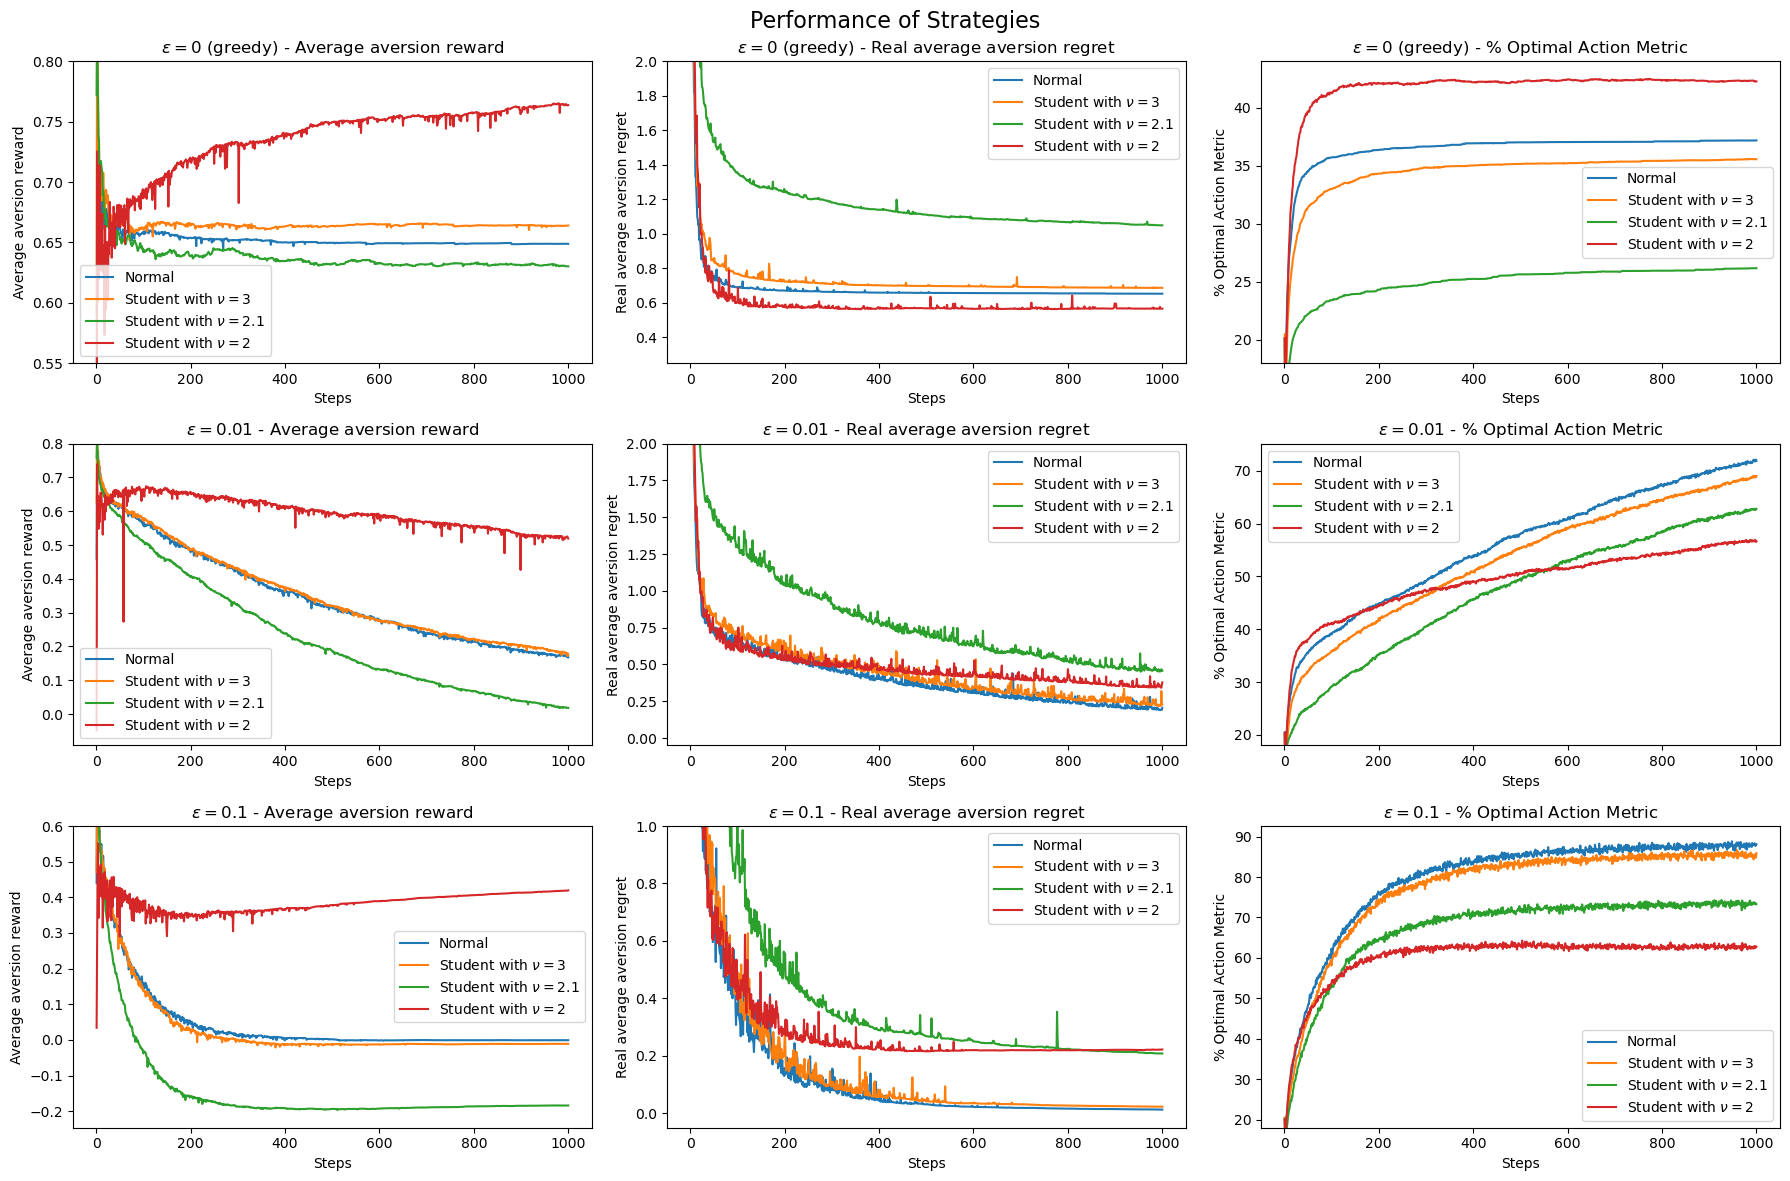
\includegraphics[scale=0.13,center]{images/theory_images/epsilon_greedy/one_strat.png}
    \end{frame}
    \begin{frame}{Результаты -- $\epsilon$-greedy}
        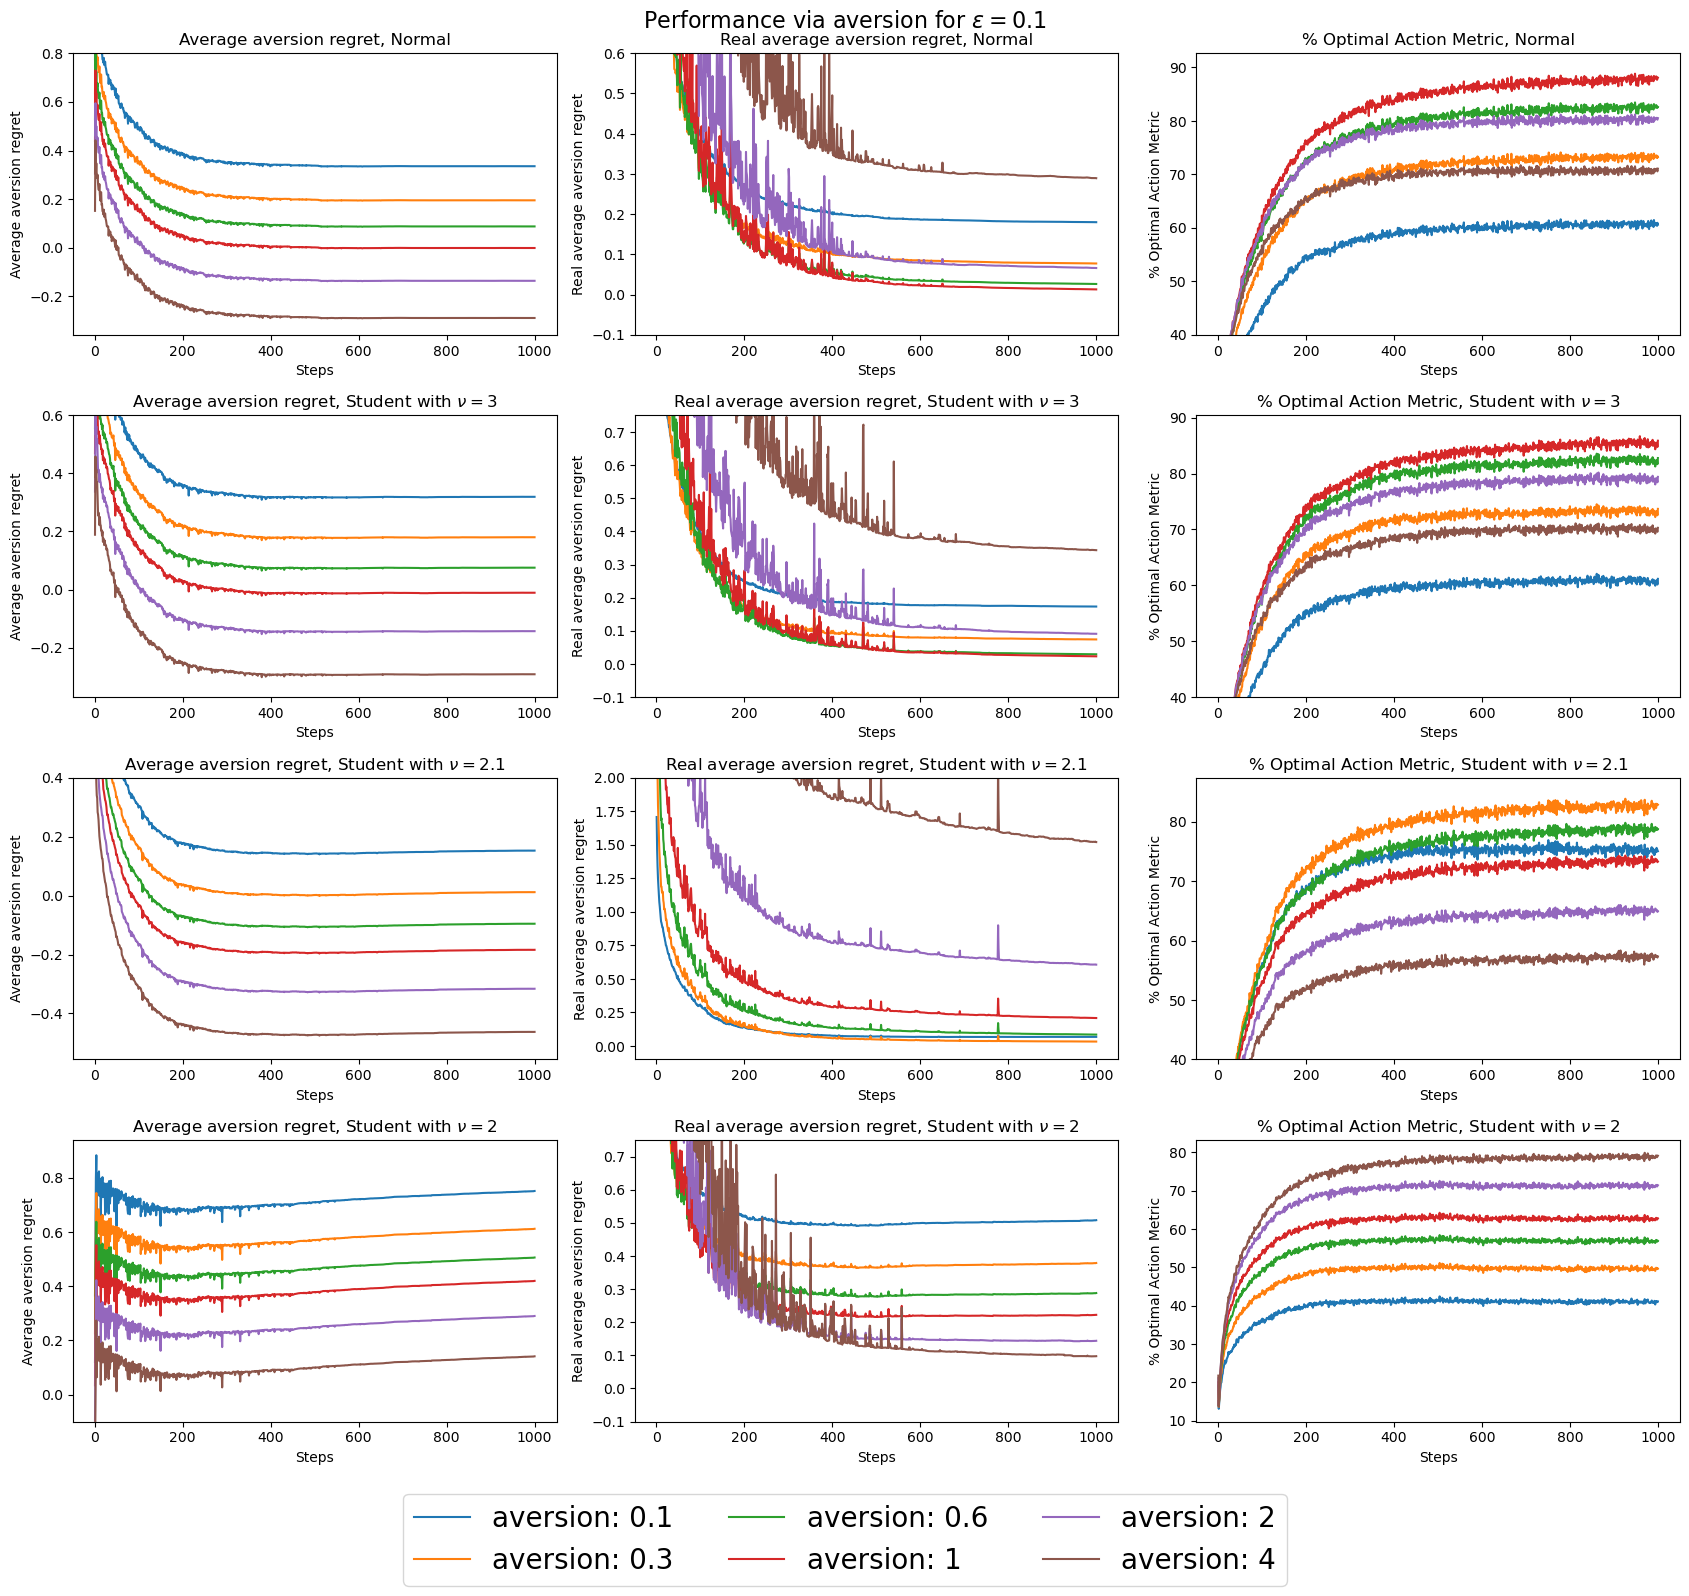
\includegraphics[scale=0.13,center]{images/theory_images/epsilon_greedy/avers_distr.png}
    \end{frame}
    \begin{frame}{Результаты -- $\epsilon$-greedy}
        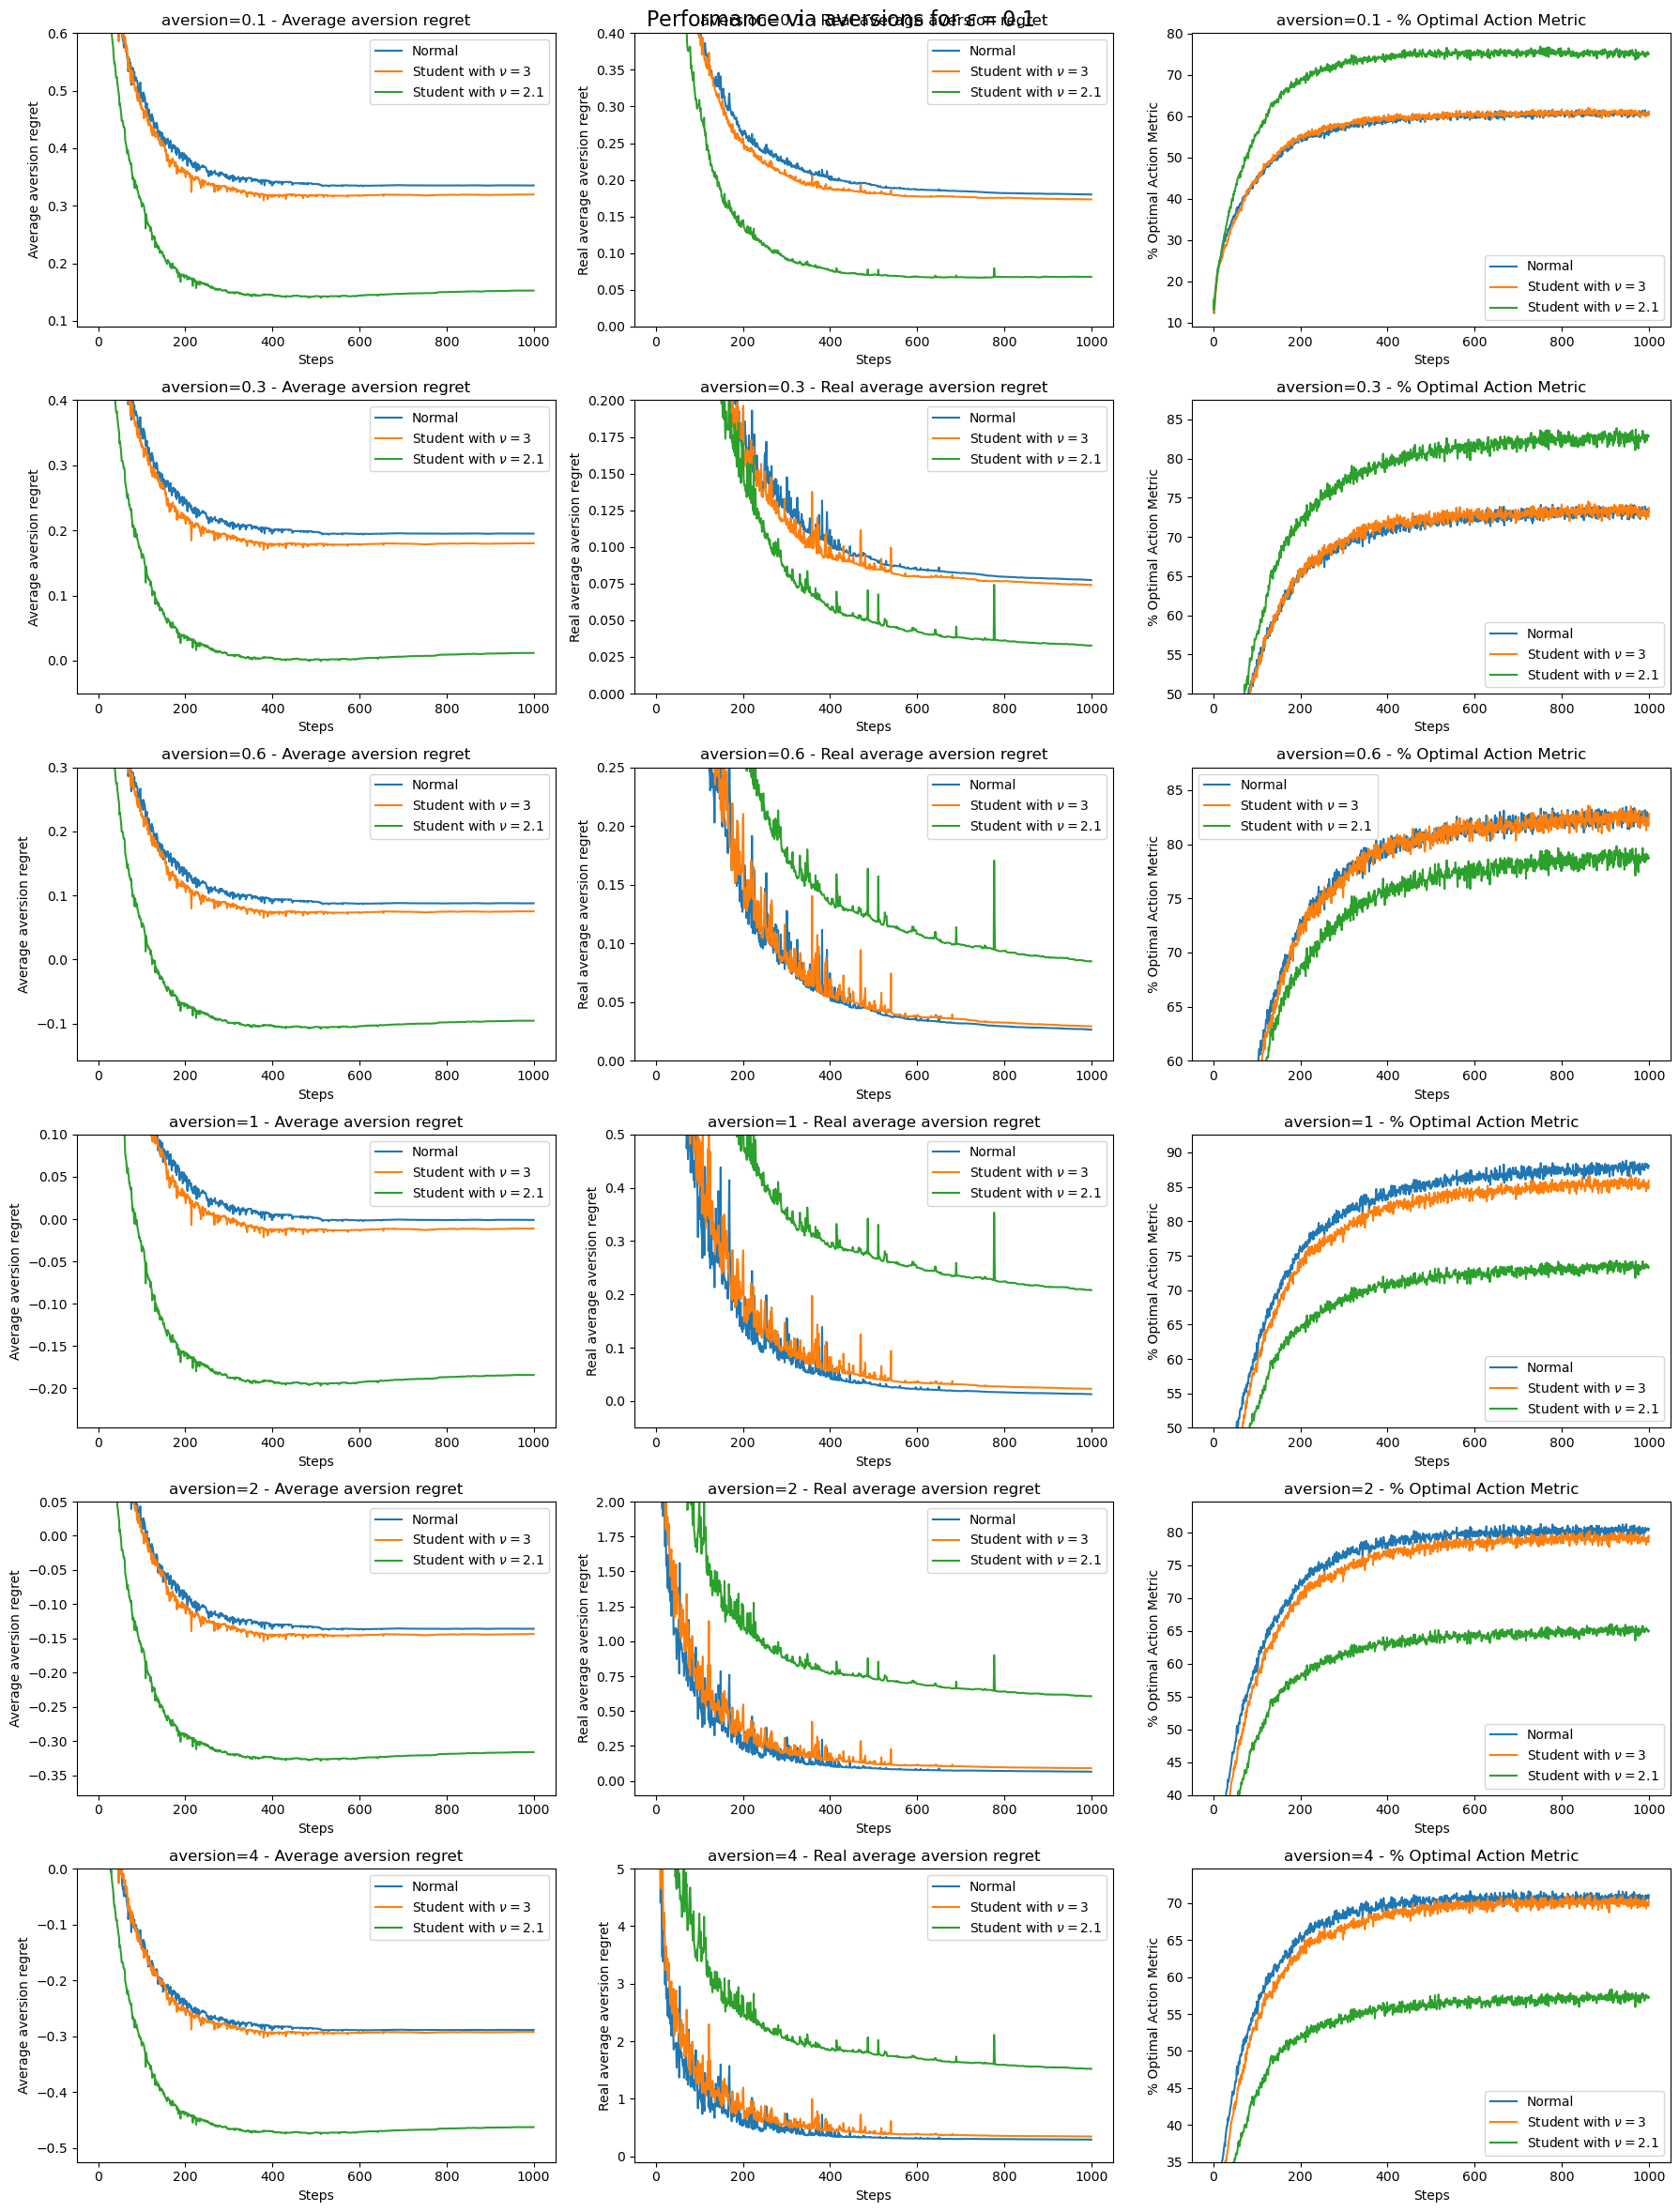
\includegraphics[scale=0.13,center]{images/theory_images/epsilon_greedy/avers_avers.png}
    \end{frame}
    \begin{frame}{Результаты -- $\epsilon$-greedy}
        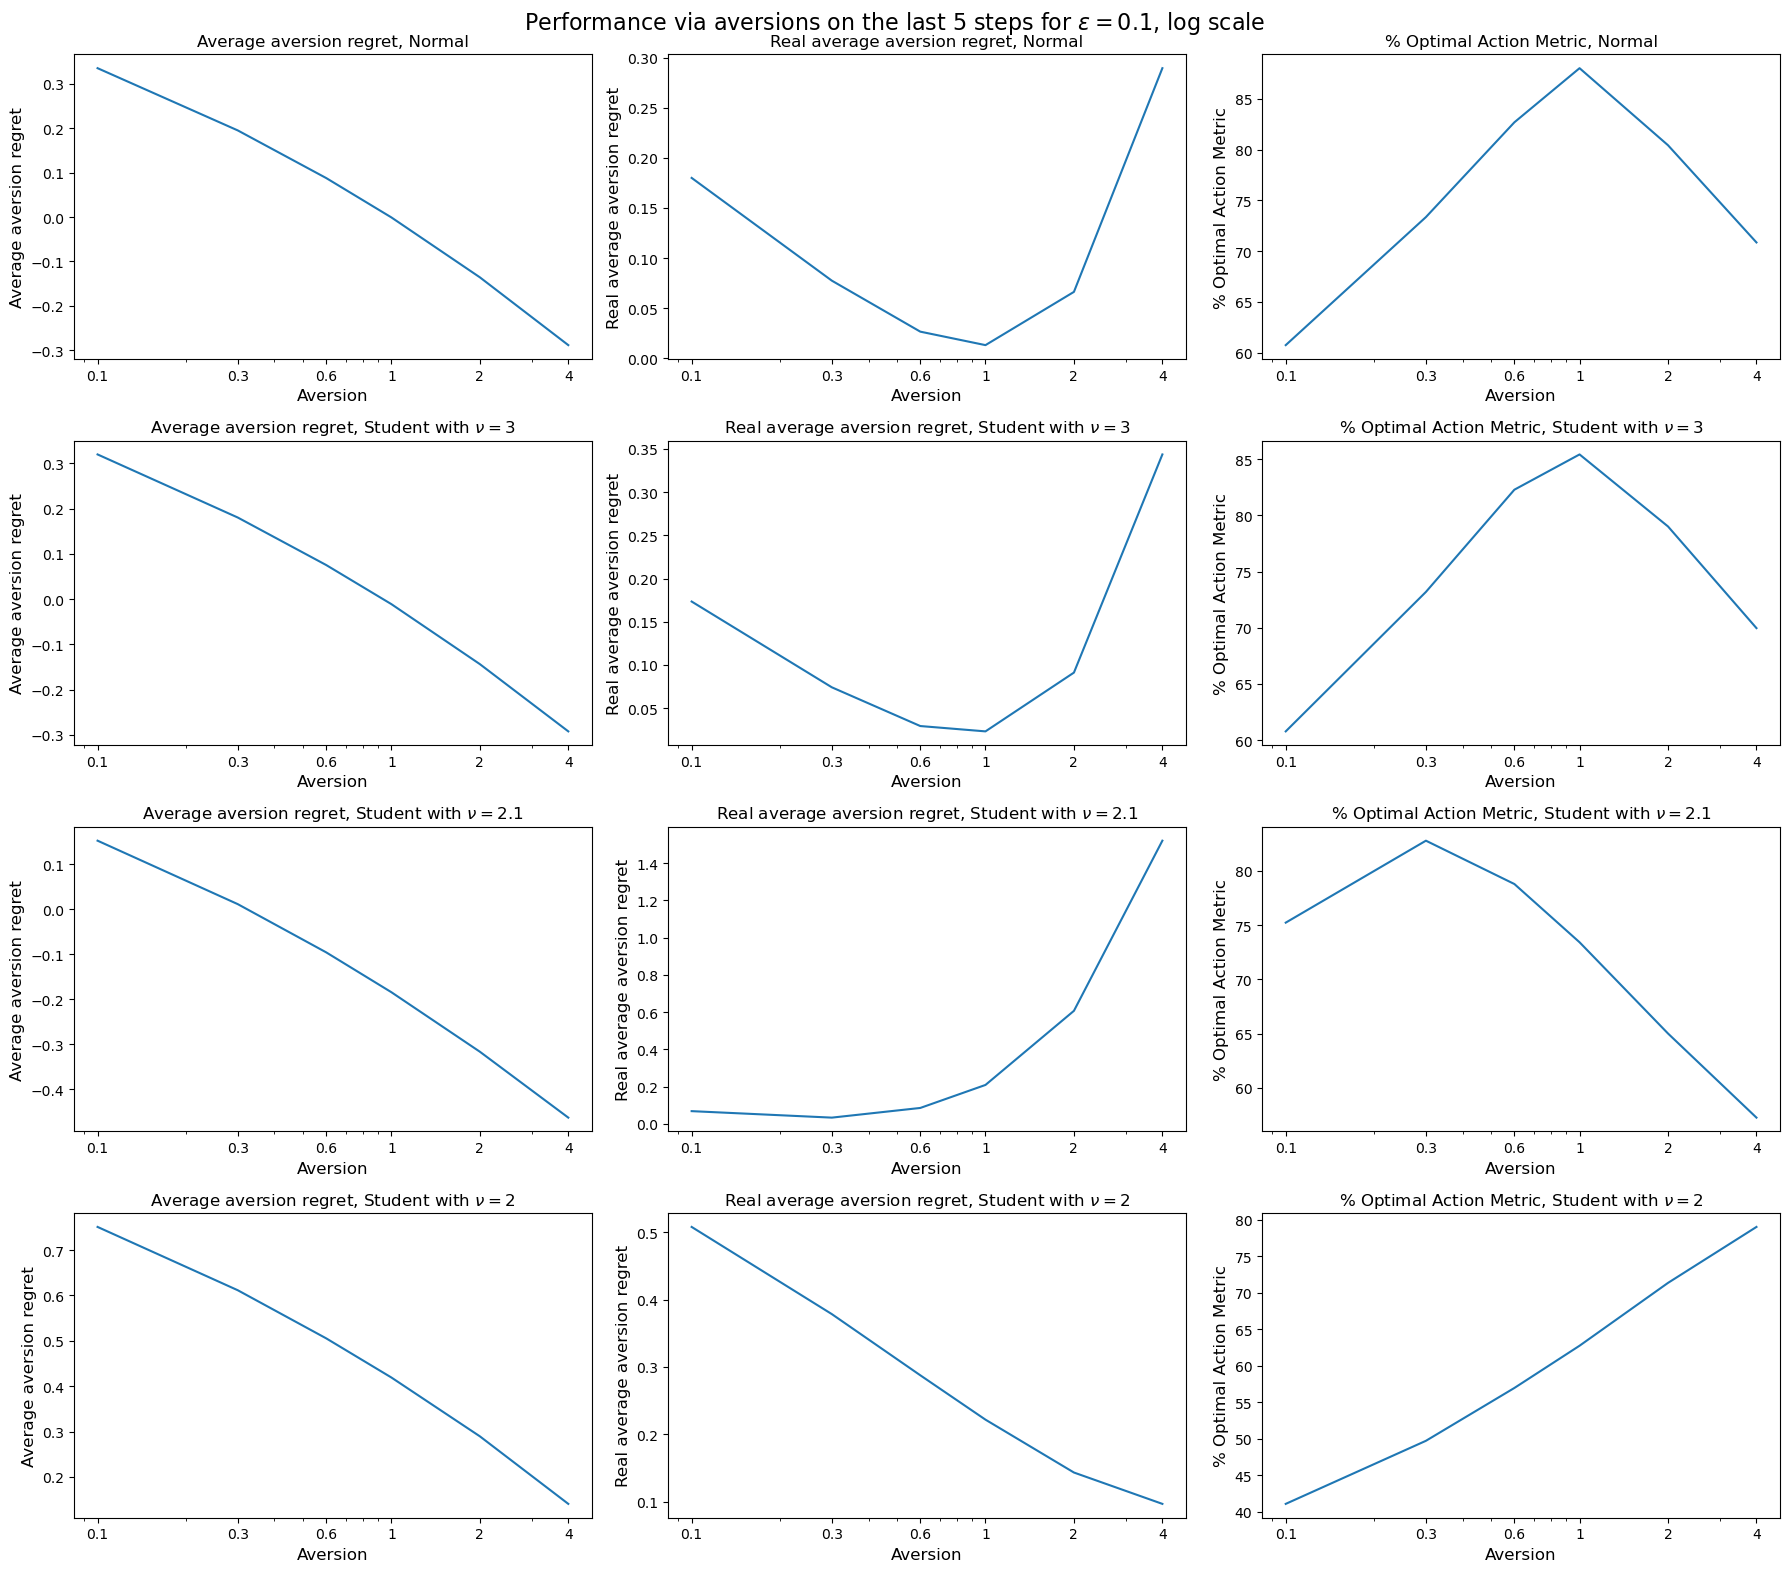
\includegraphics[scale=0.13,center]{images/theory_images/epsilon_greedy/avers_last.png}
    \end{frame}
    \begin{frame}{Результаты -- adaptive $\epsilon$}
        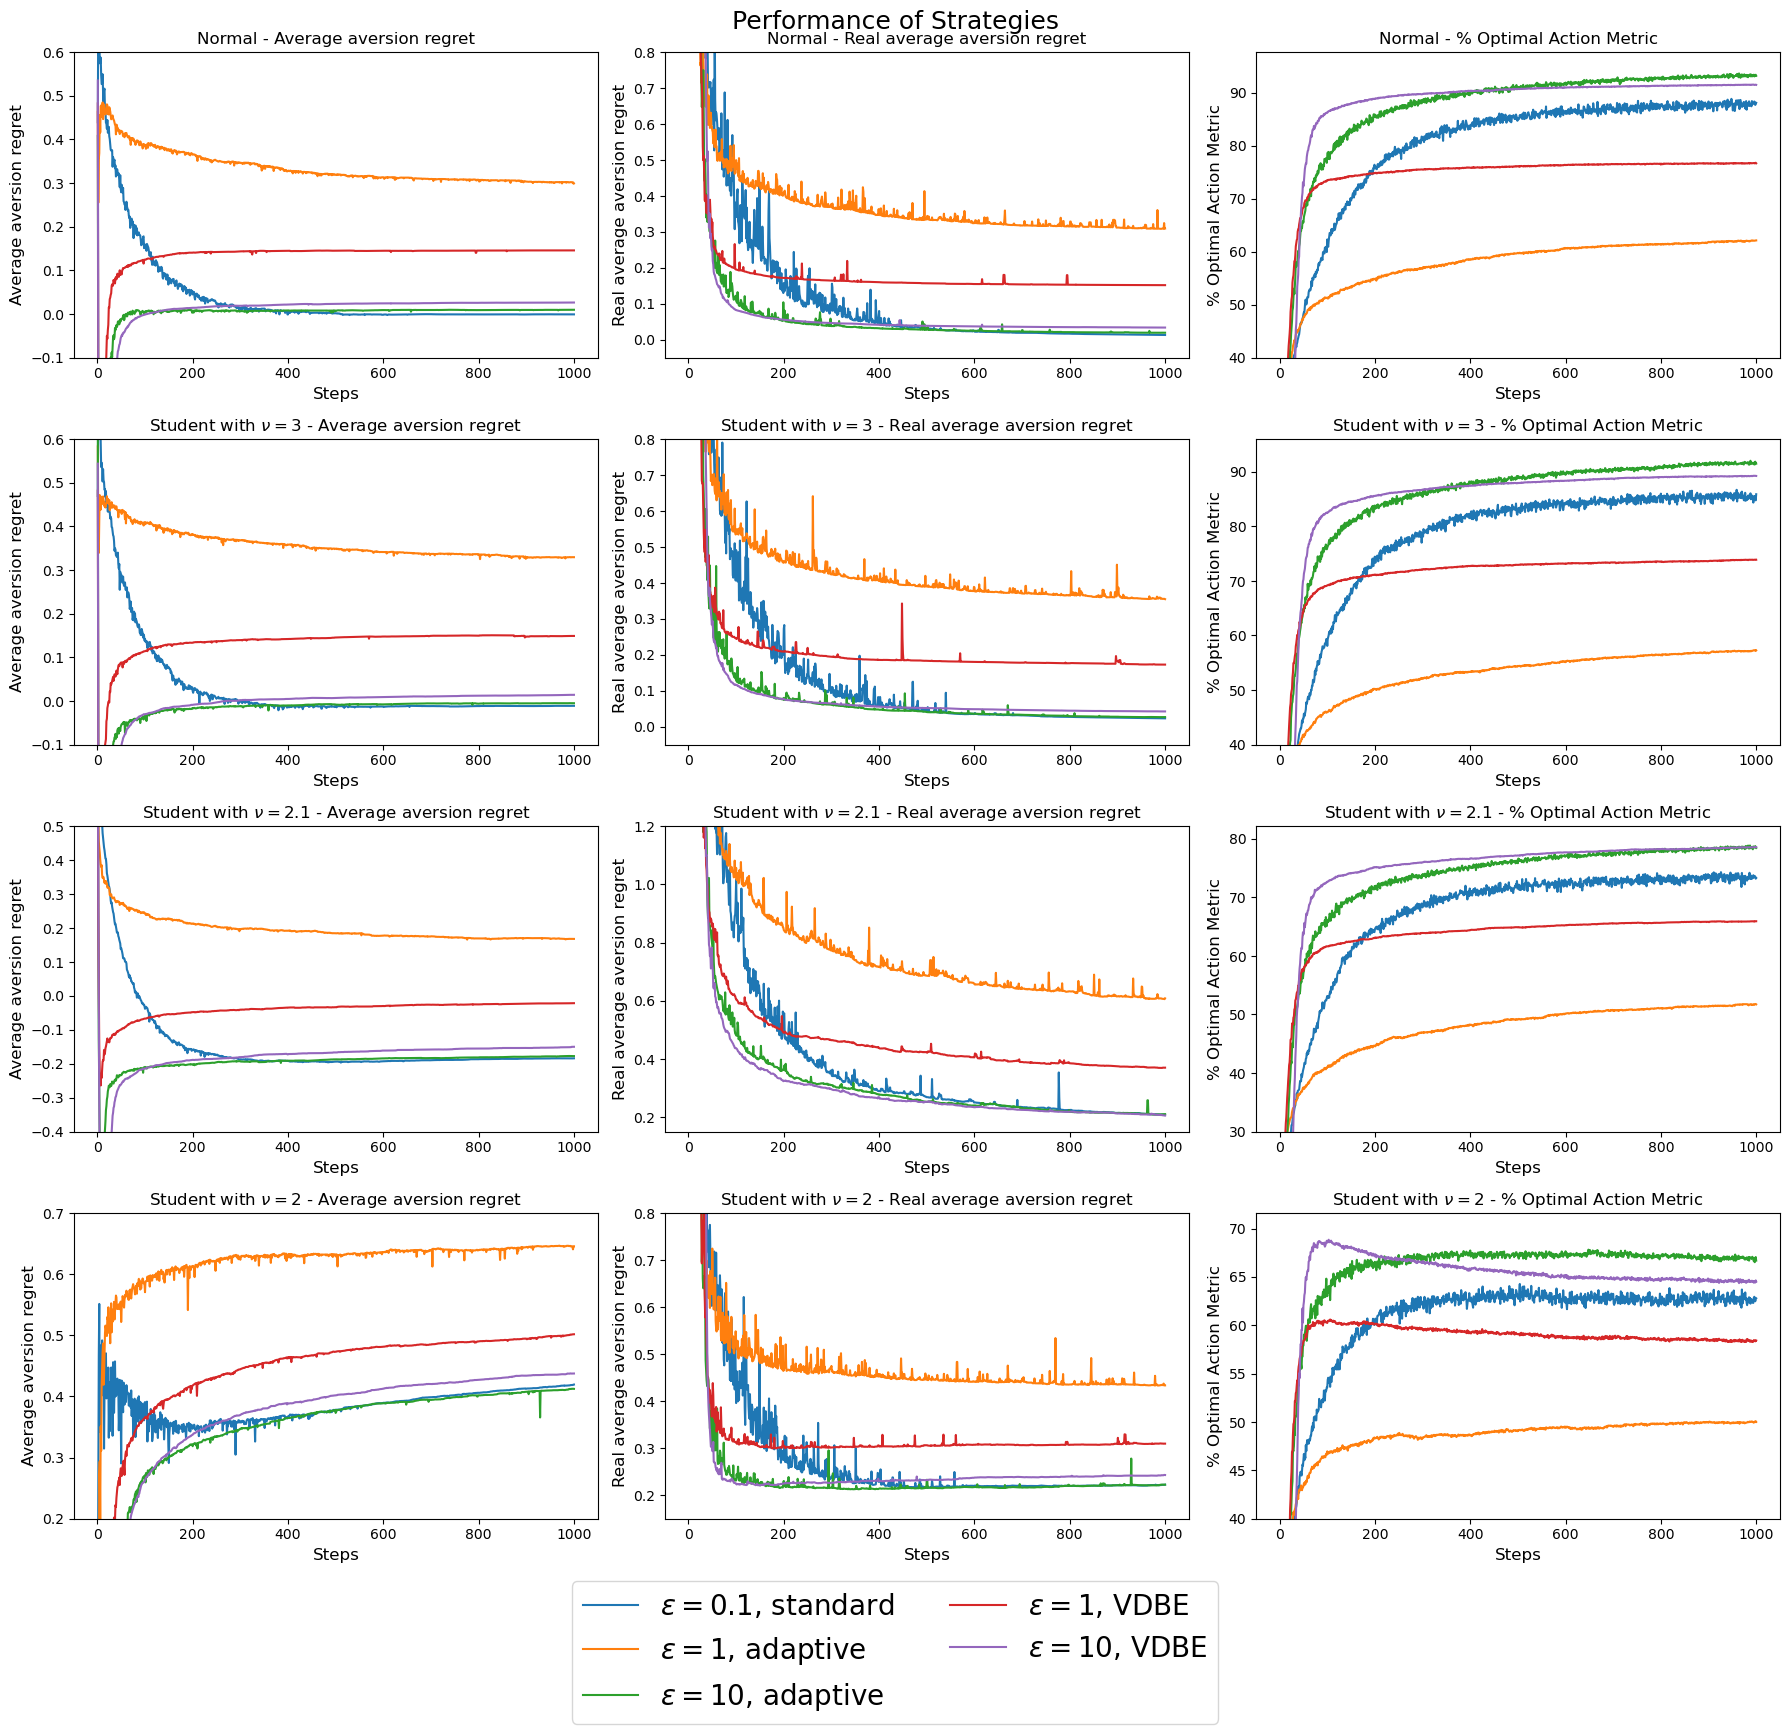
\includegraphics[scale=0.13,center]{images/theory_images/adaptive_epsilon/one_distr.png}
    \end{frame}
    \begin{frame}{Результаты -- adaptive $\epsilon$}
        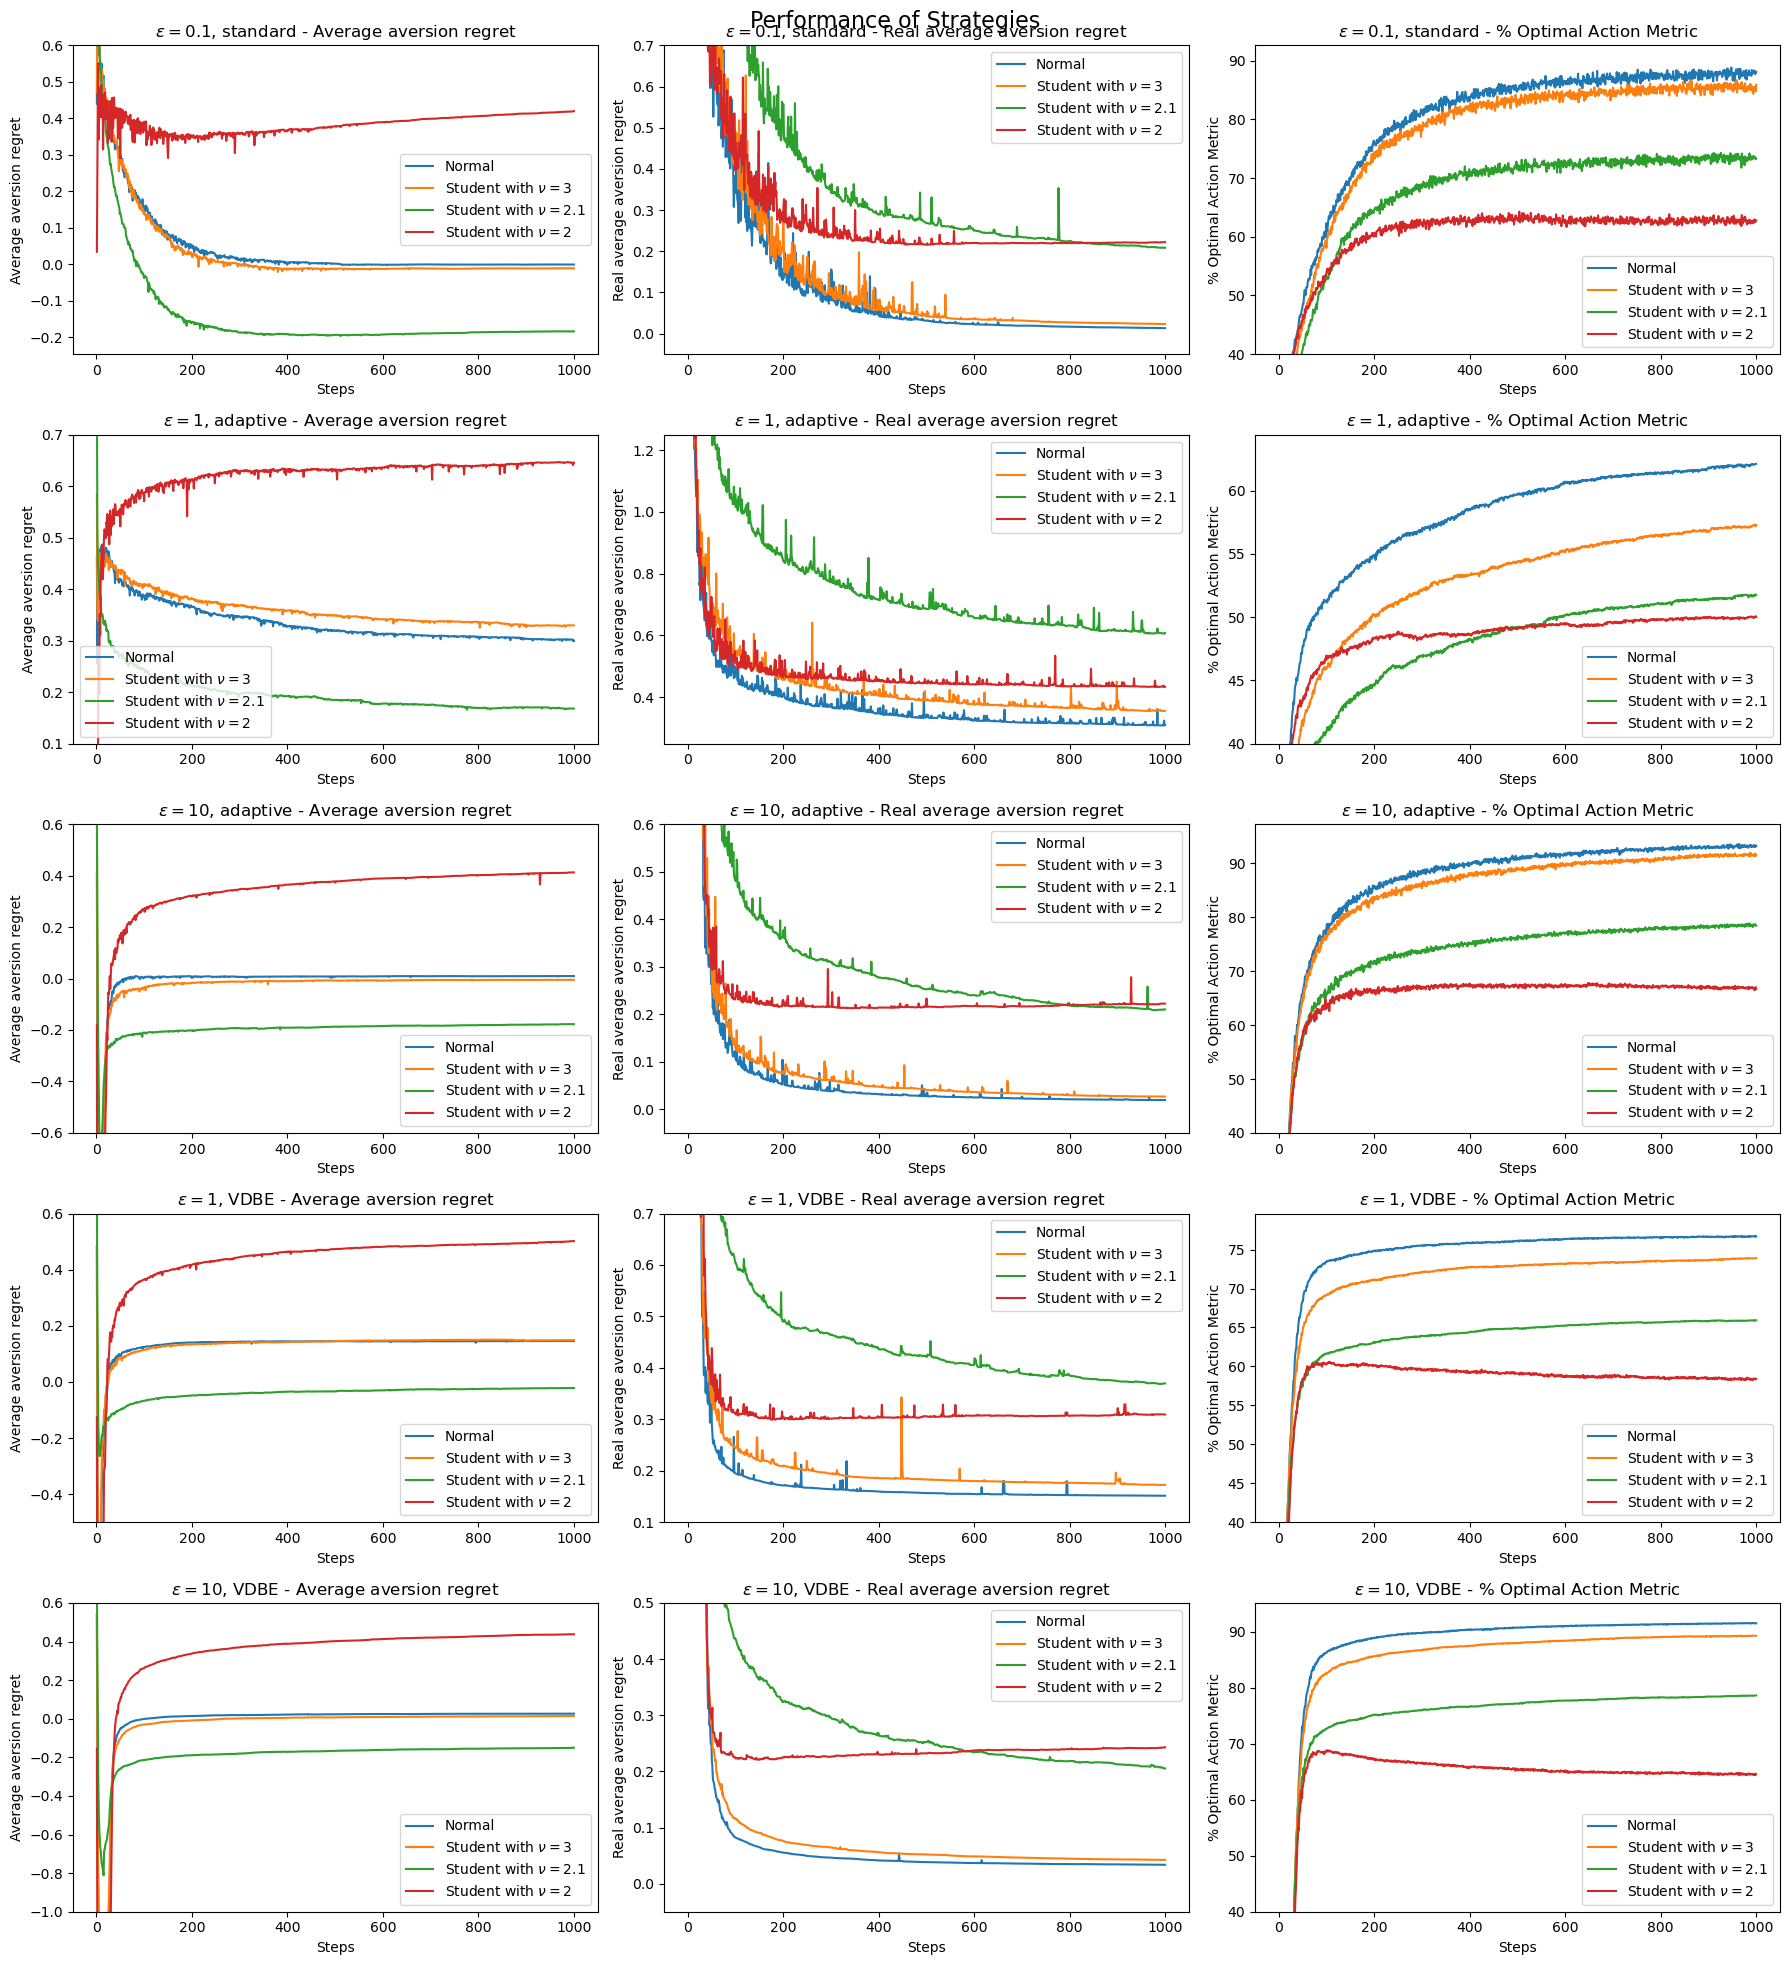
\includegraphics[scale=0.13,center]{images/theory_images/adaptive_epsilon/one_strat.png}
    \end{frame}
    \begin{frame}{Результаты -- adaptive $\epsilon$}
        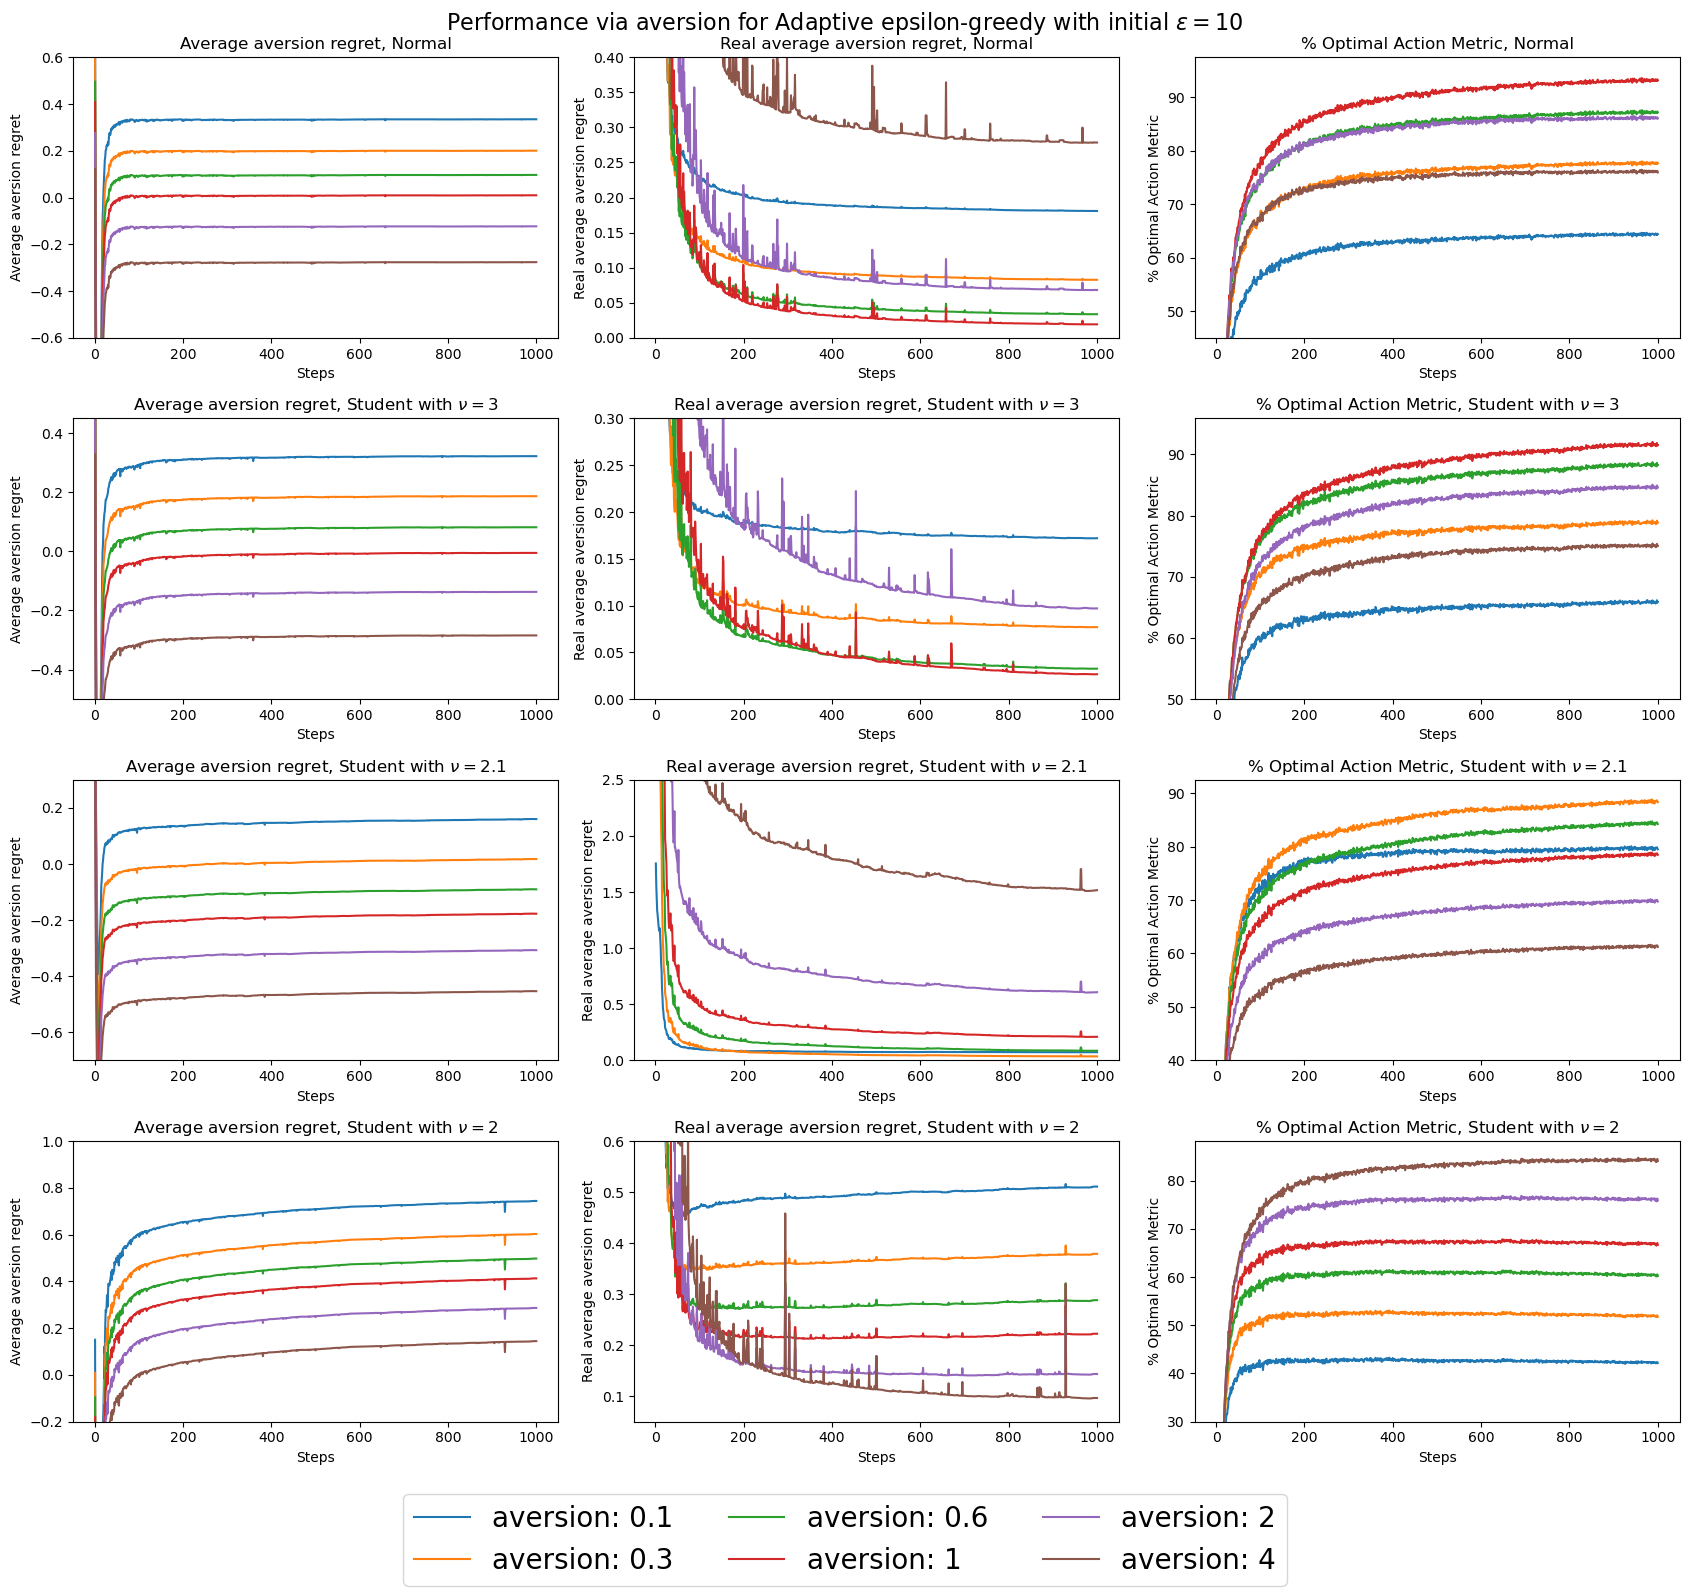
\includegraphics[scale=0.13,center]{images/theory_images/adaptive_epsilon/avers_distr.png}
    \end{frame}
    \begin{frame}{Результаты -- adaptive $\epsilon$}
        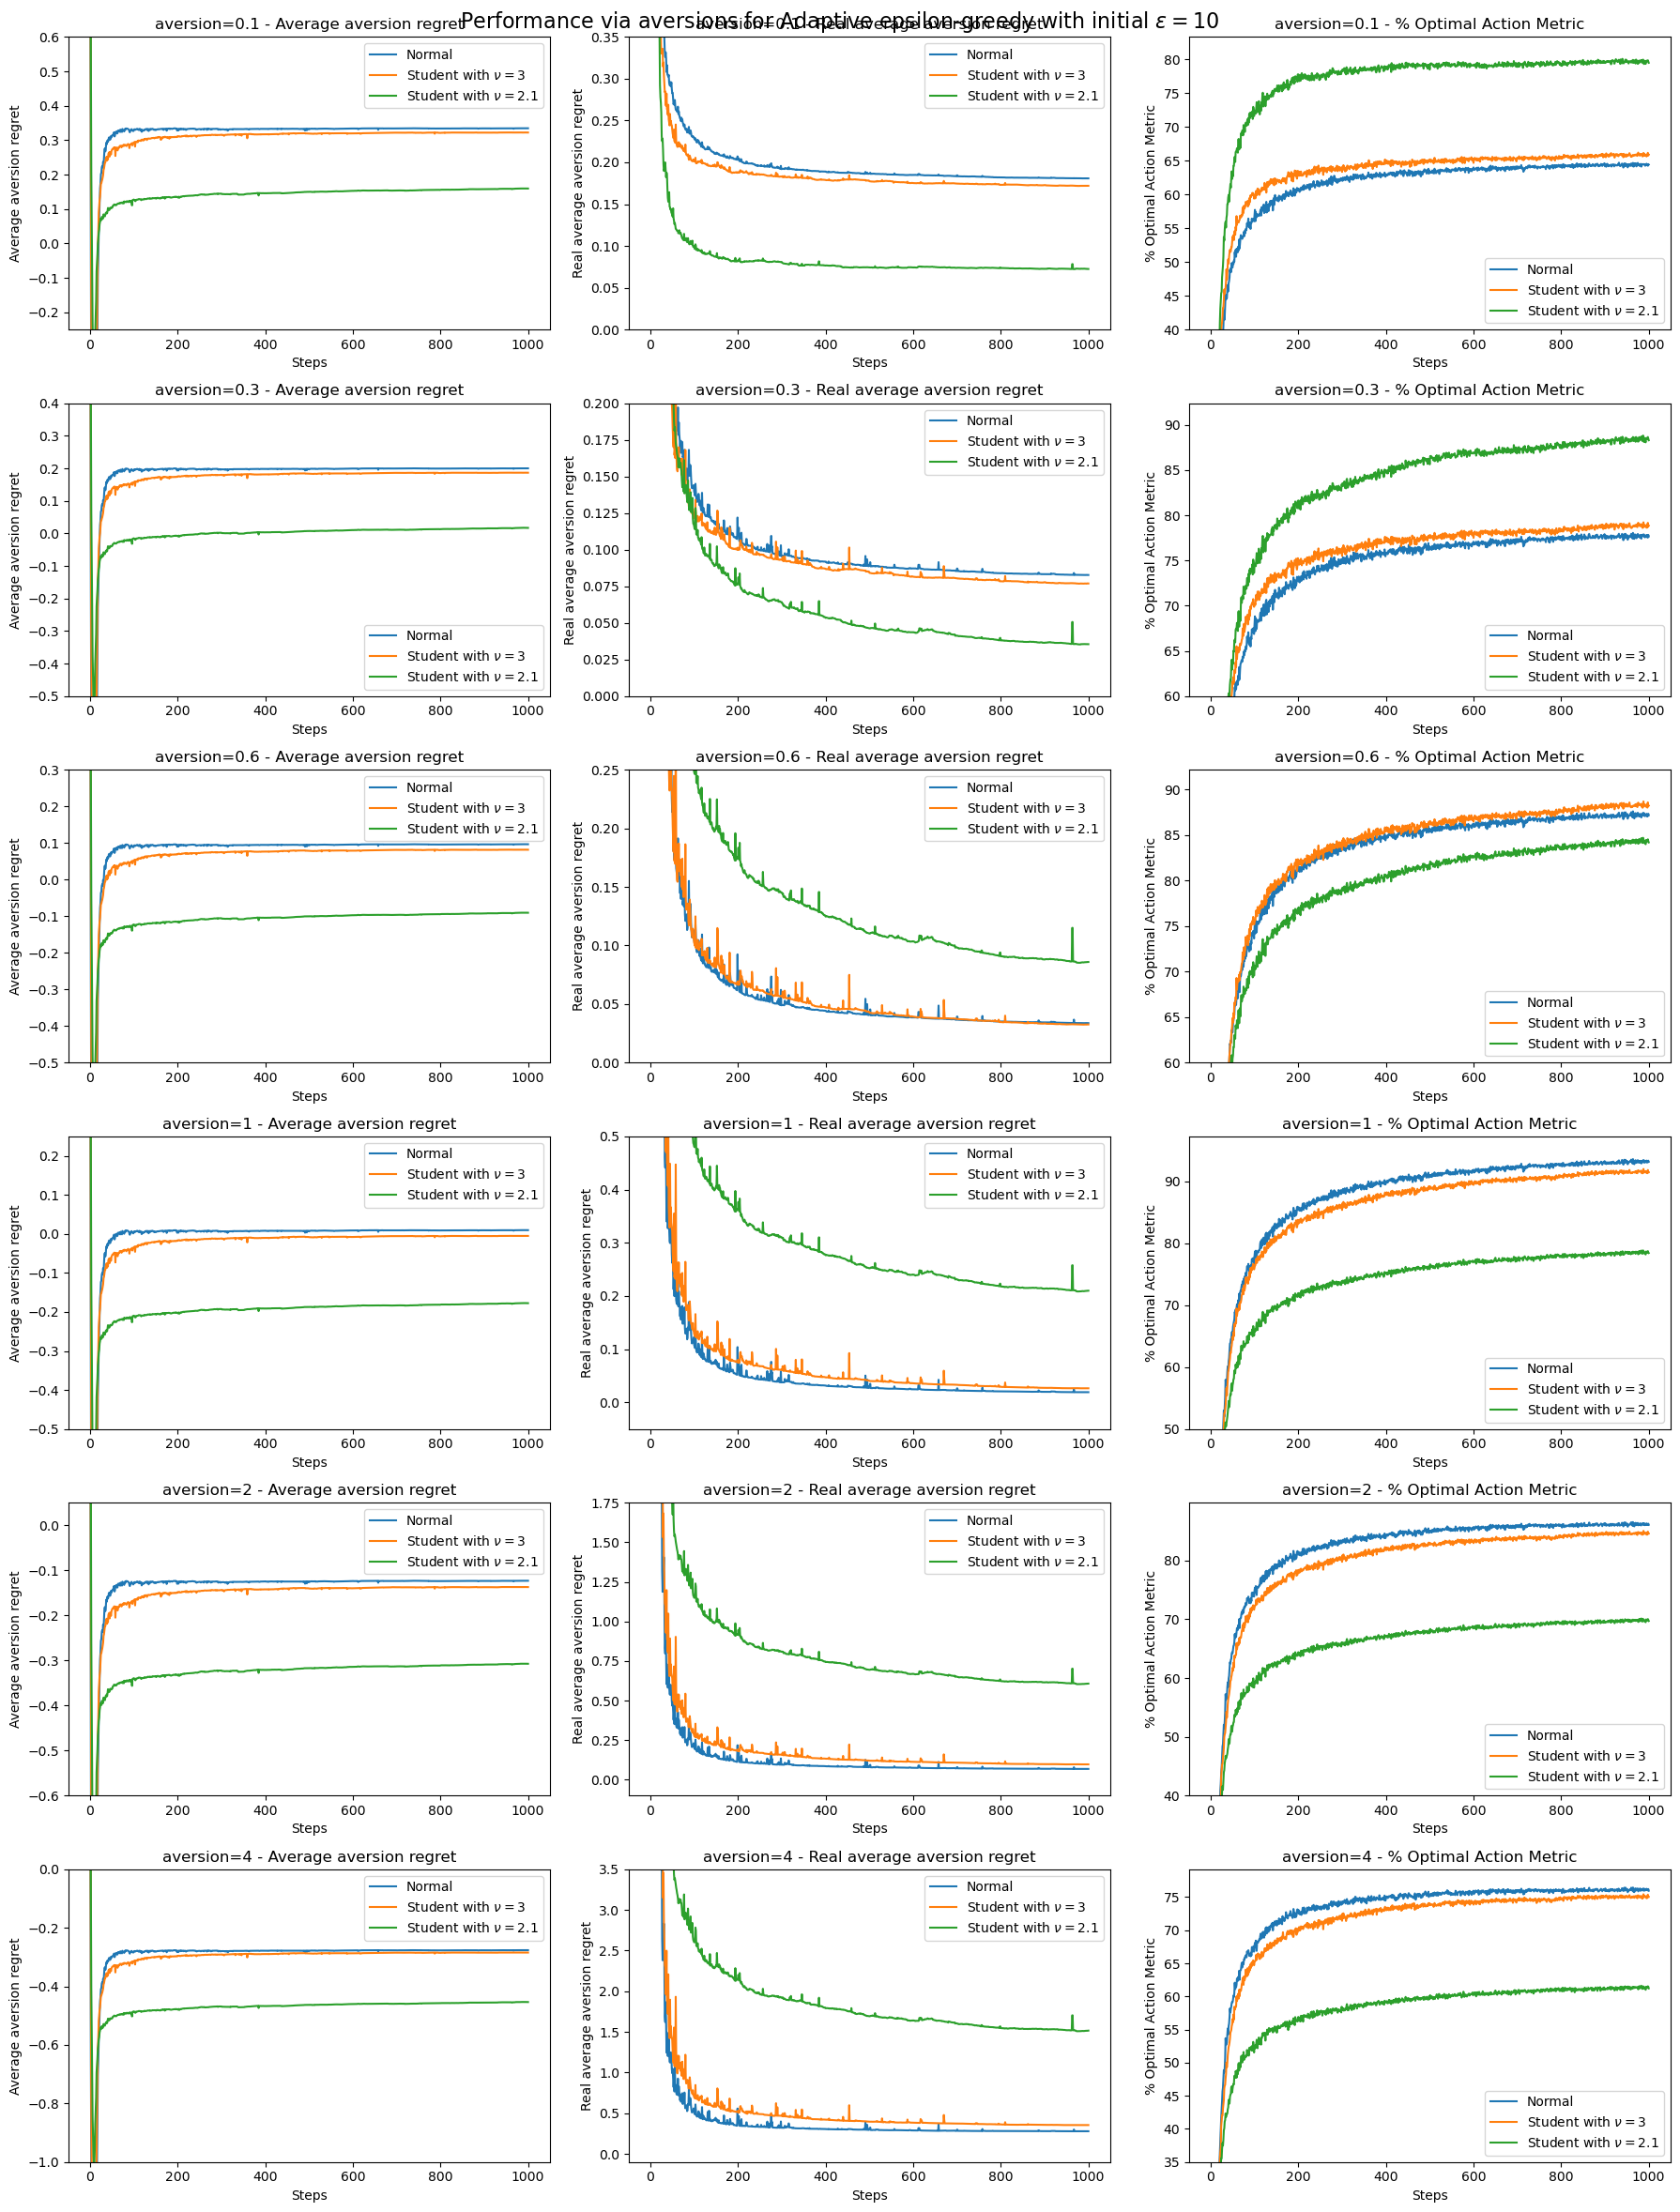
\includegraphics[scale=0.13,center]{images/theory_images/adaptive_epsilon/avers_avers.png}
    \end{frame}
    \begin{frame}{Результаты -- adaptive $\epsilon$}
        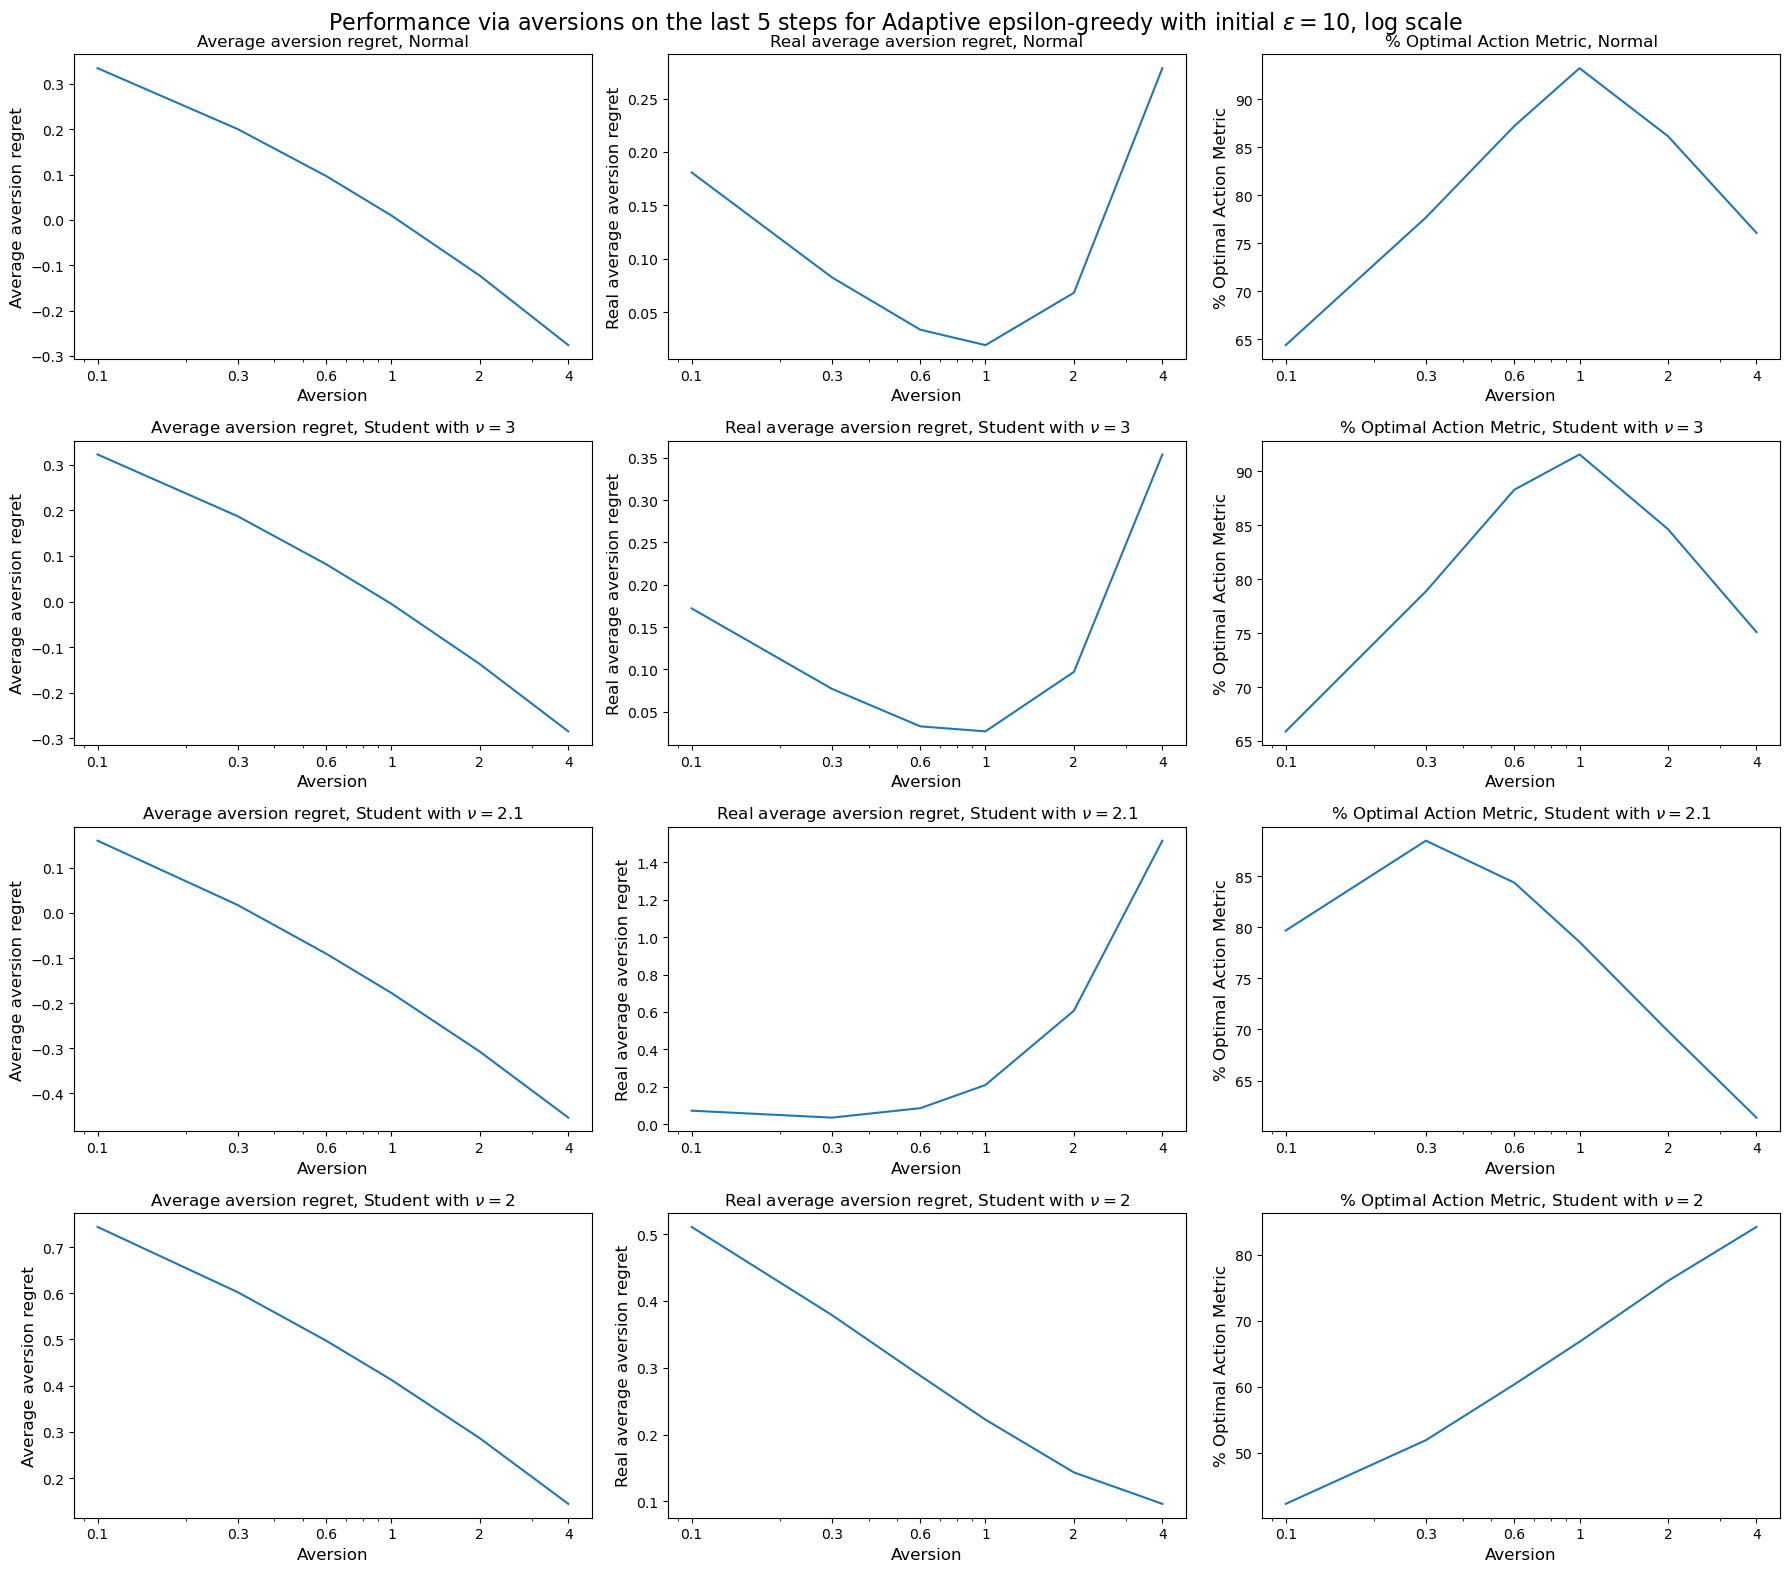
\includegraphics[scale=0.13,center]{images/theory_images/adaptive_epsilon/avers_last.png}
    \end{frame}
    \begin{frame}{Результаты -- positive initialization}
        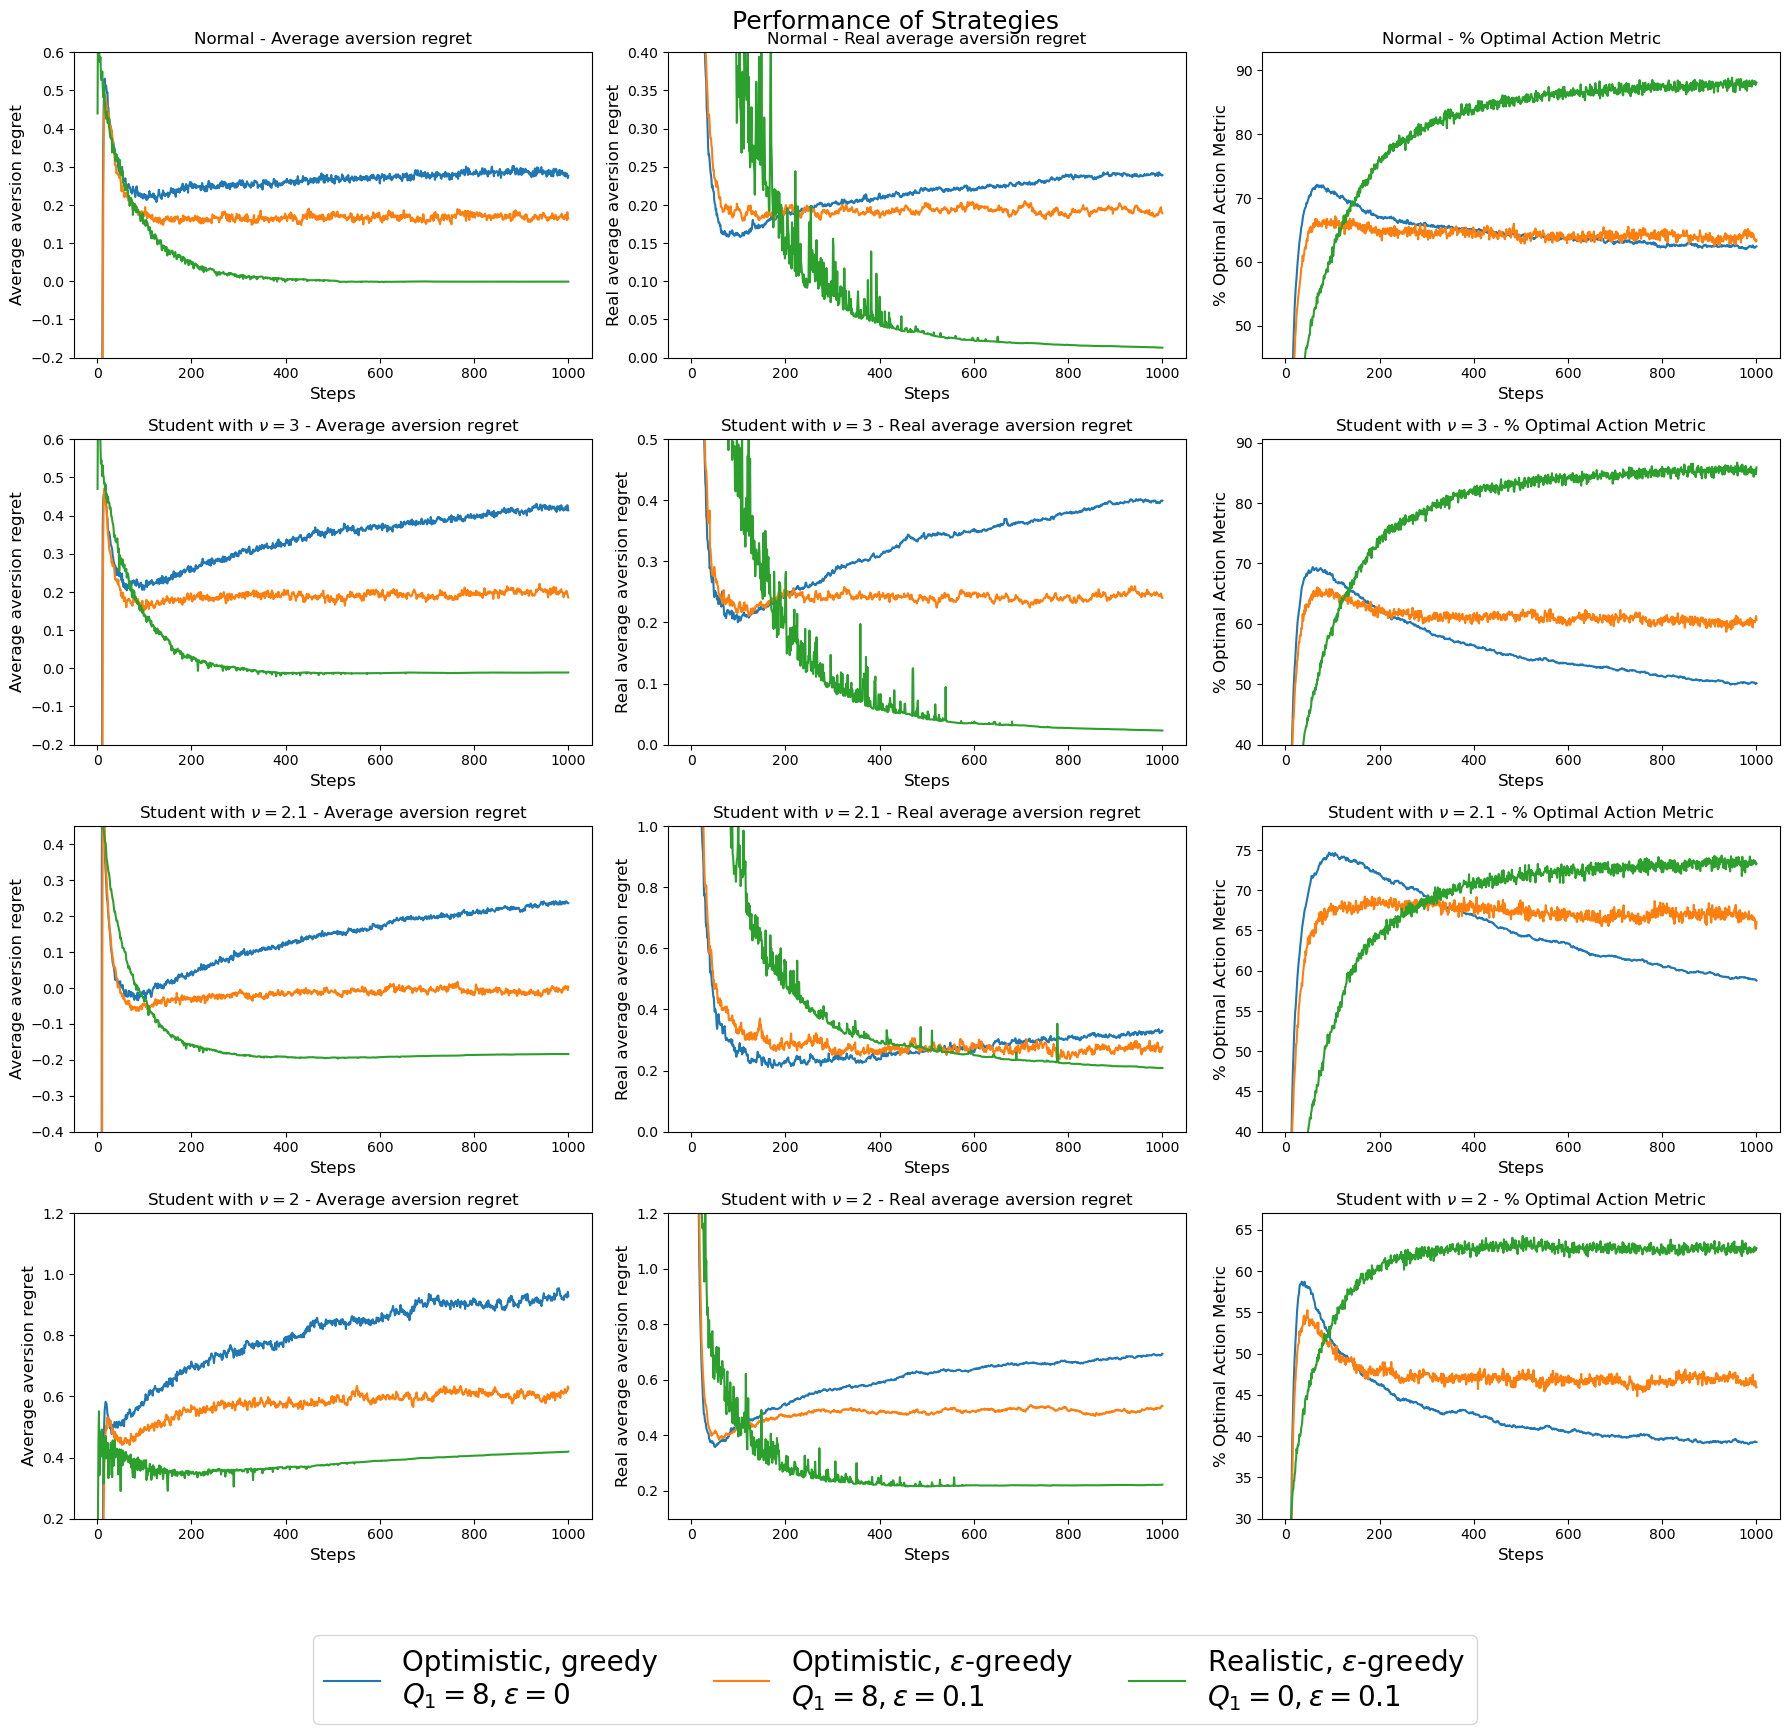
\includegraphics[scale=0.13,center]{images/theory_images/positive_init/one_distr.png}
    \end{frame}
    \begin{frame}{Результаты -- positive initialization}
        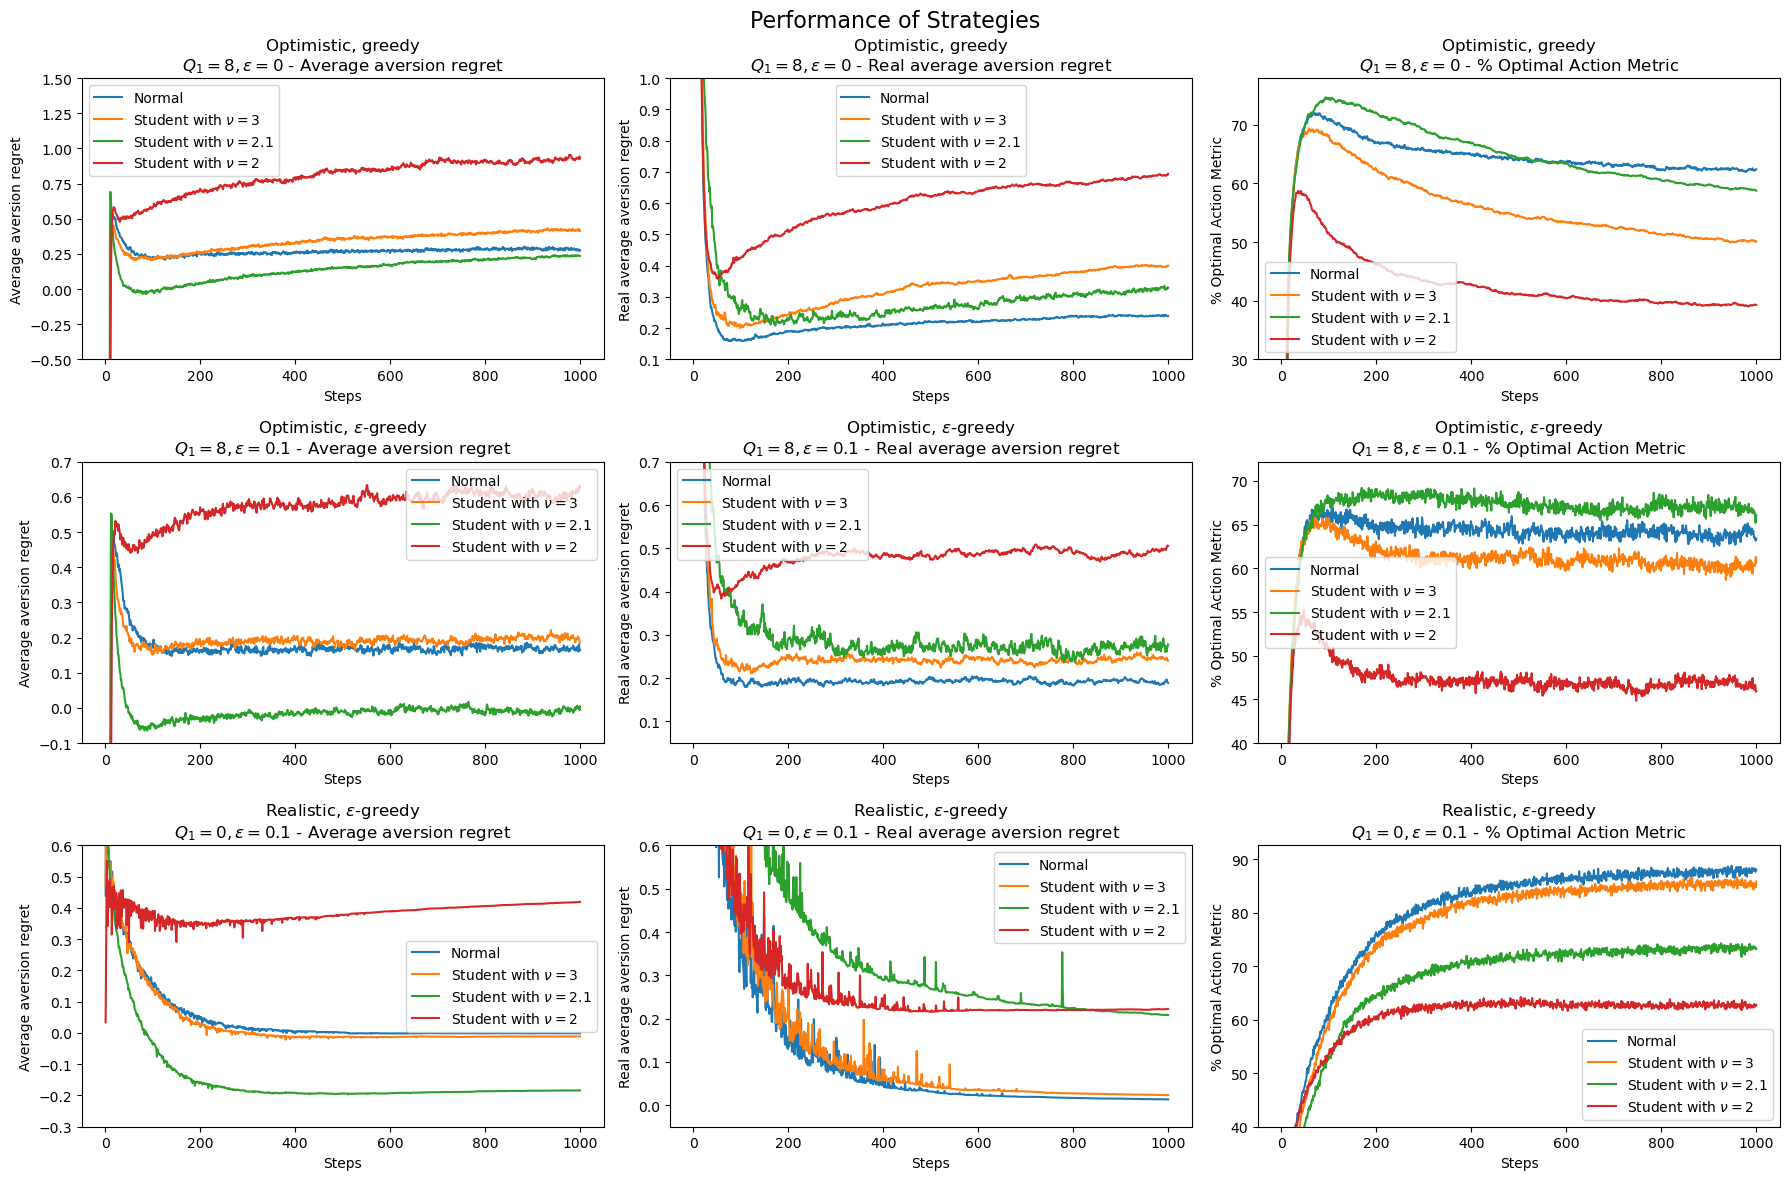
\includegraphics[scale=0.13,center]{images/theory_images/positive_init/one_strat.png}
    \end{frame}
    \begin{frame}{Результаты -- UCB}
        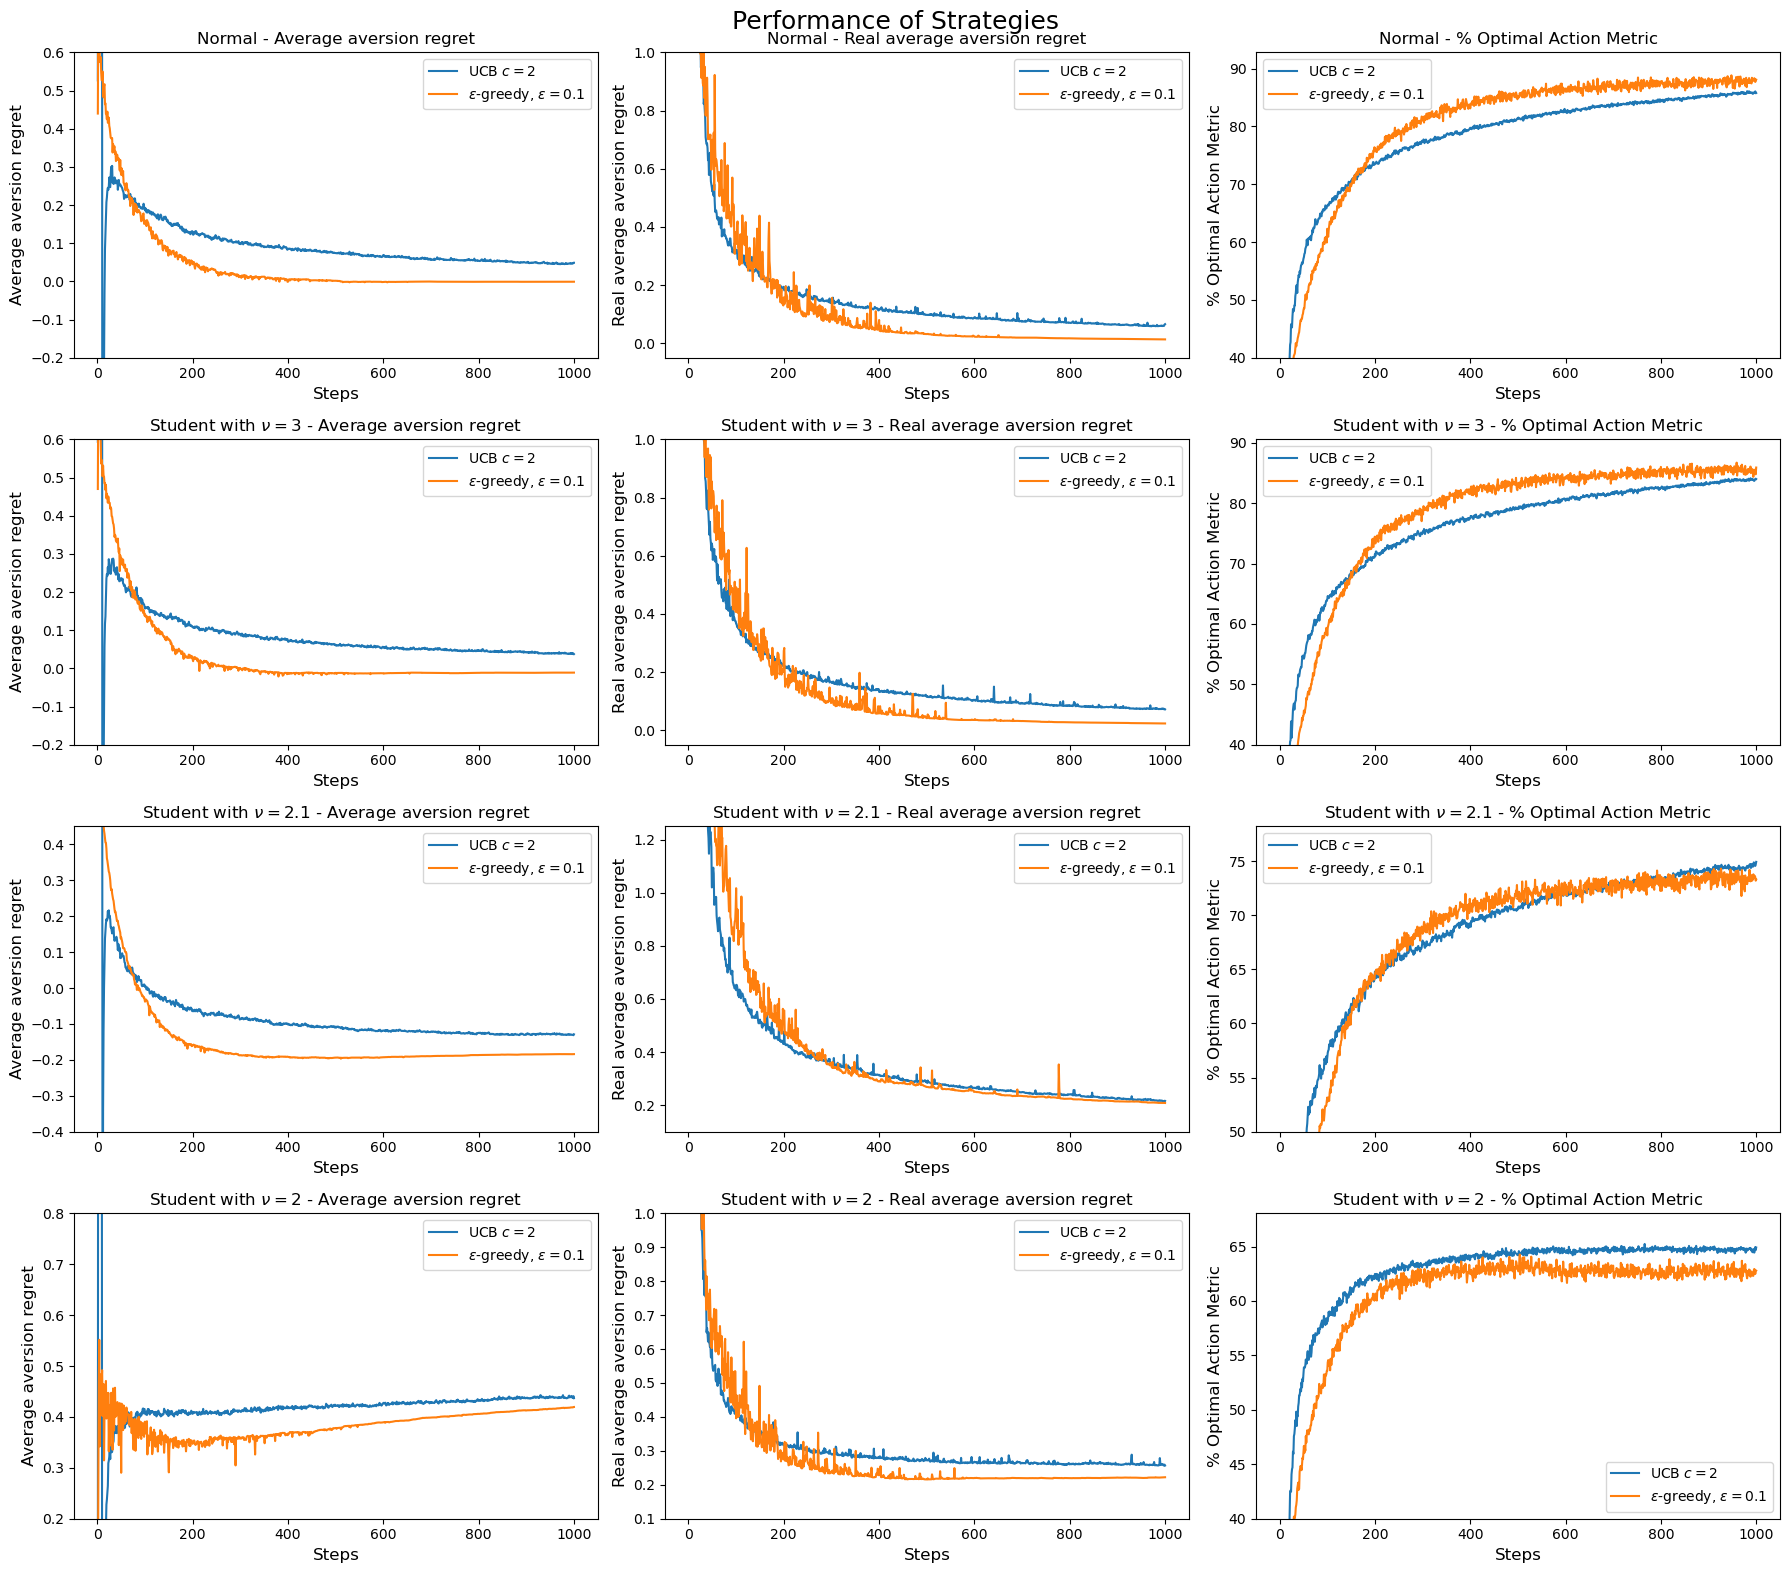
\includegraphics[scale=0.13,center]{images/theory_images/UCB/one_distr.png}
    \end{frame}
    \begin{frame}{Результаты -- UCB}
        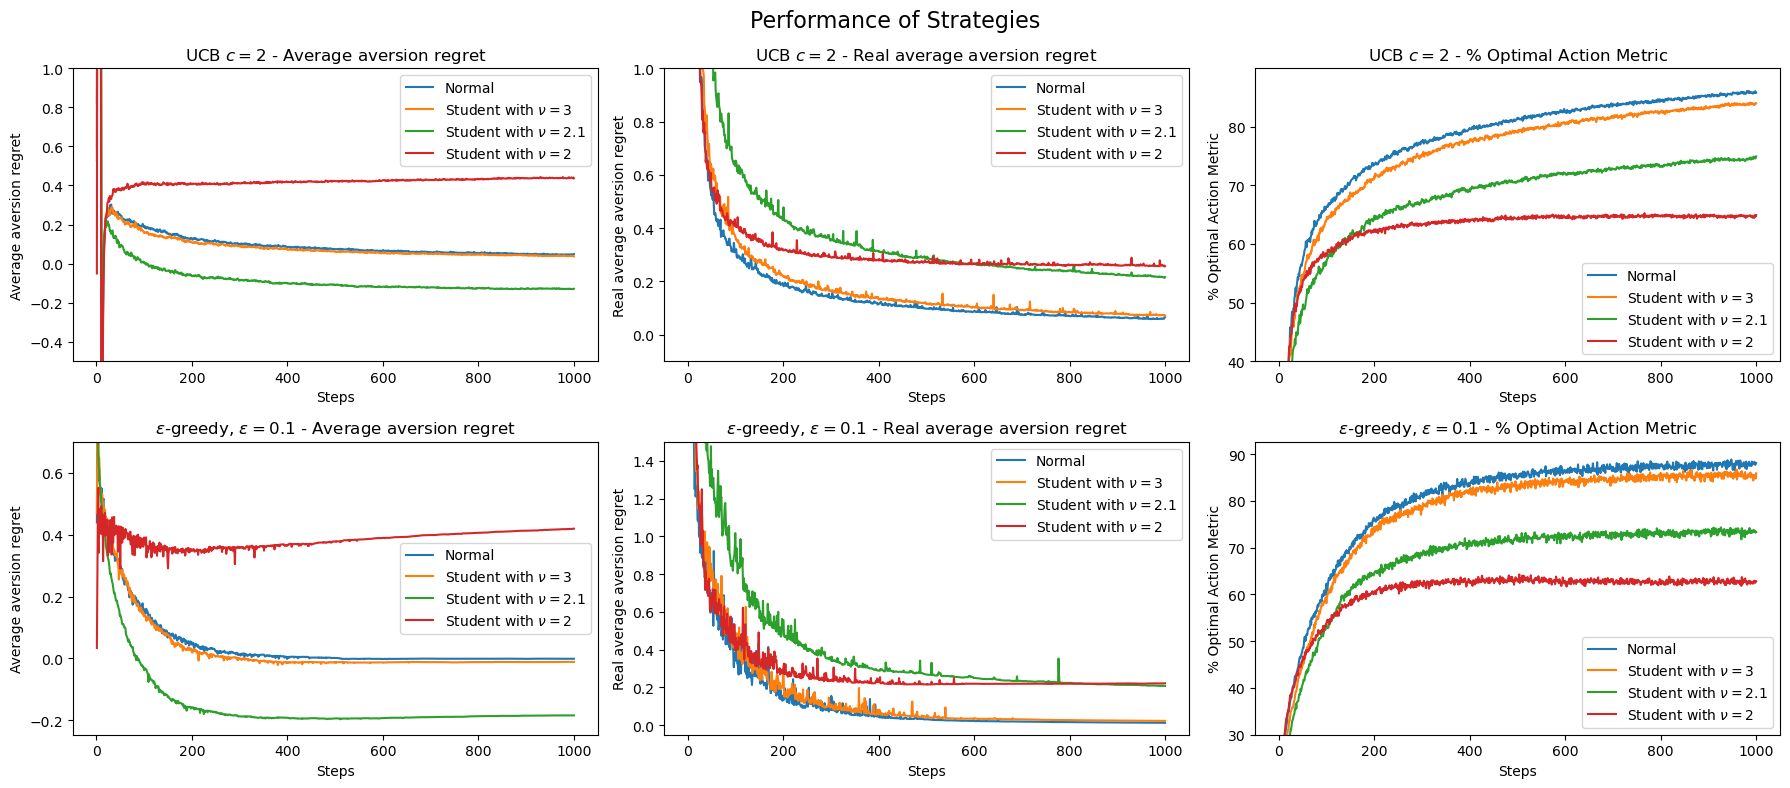
\includegraphics[scale=0.13,center]{images/theory_images/UCB/one_strat.png}
    \end{frame}
    \begin{frame}{Результаты -- UCB}
        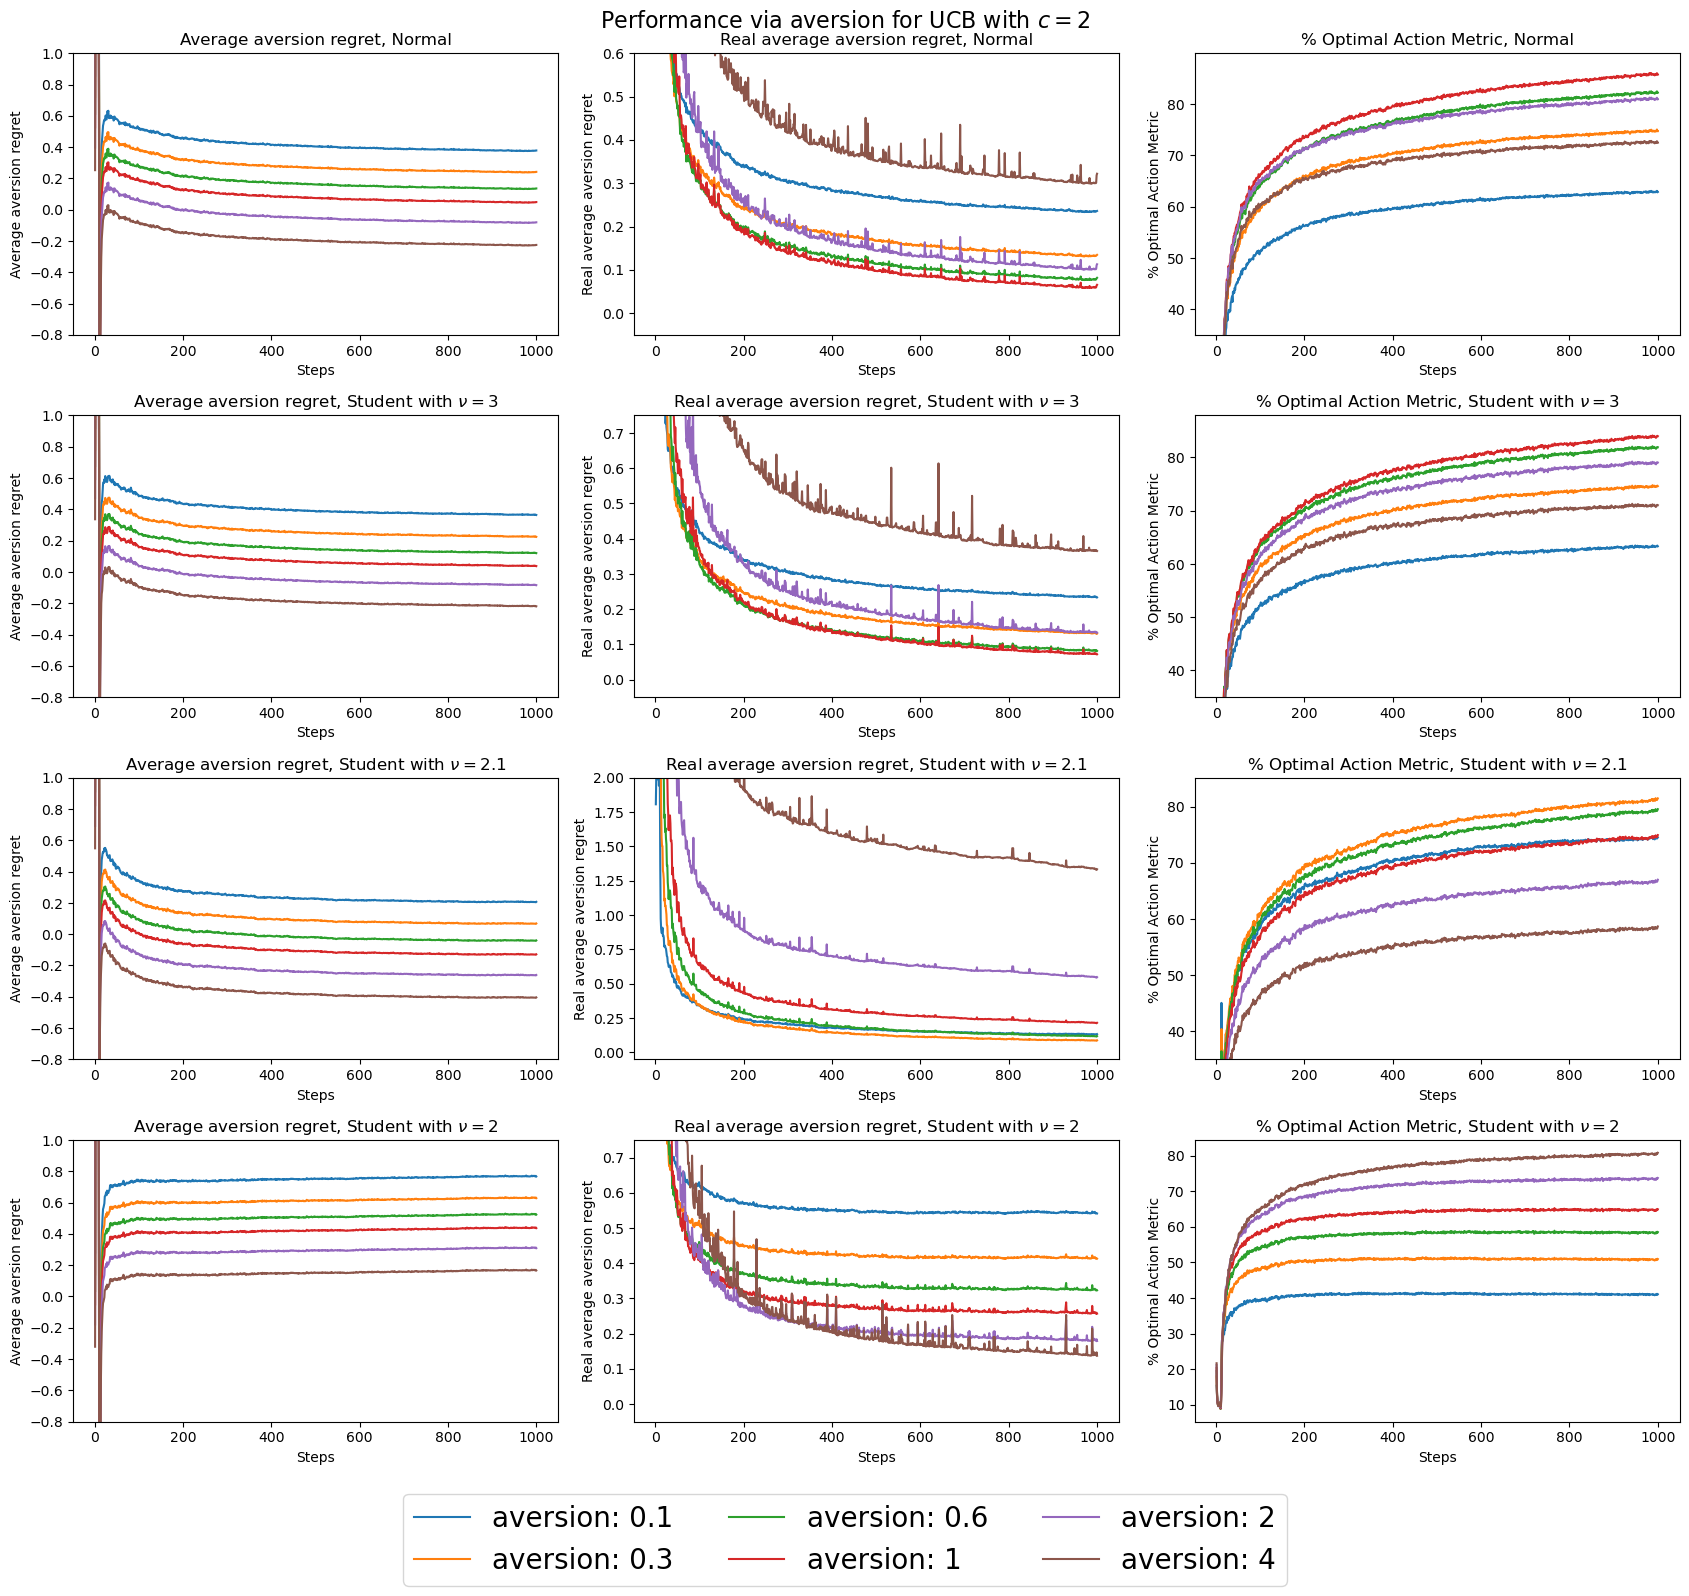
\includegraphics[scale=0.13,center]{images/theory_images/UCB/avers_distr.png}
    \end{frame}
    \begin{frame}{Результаты -- UCB}
        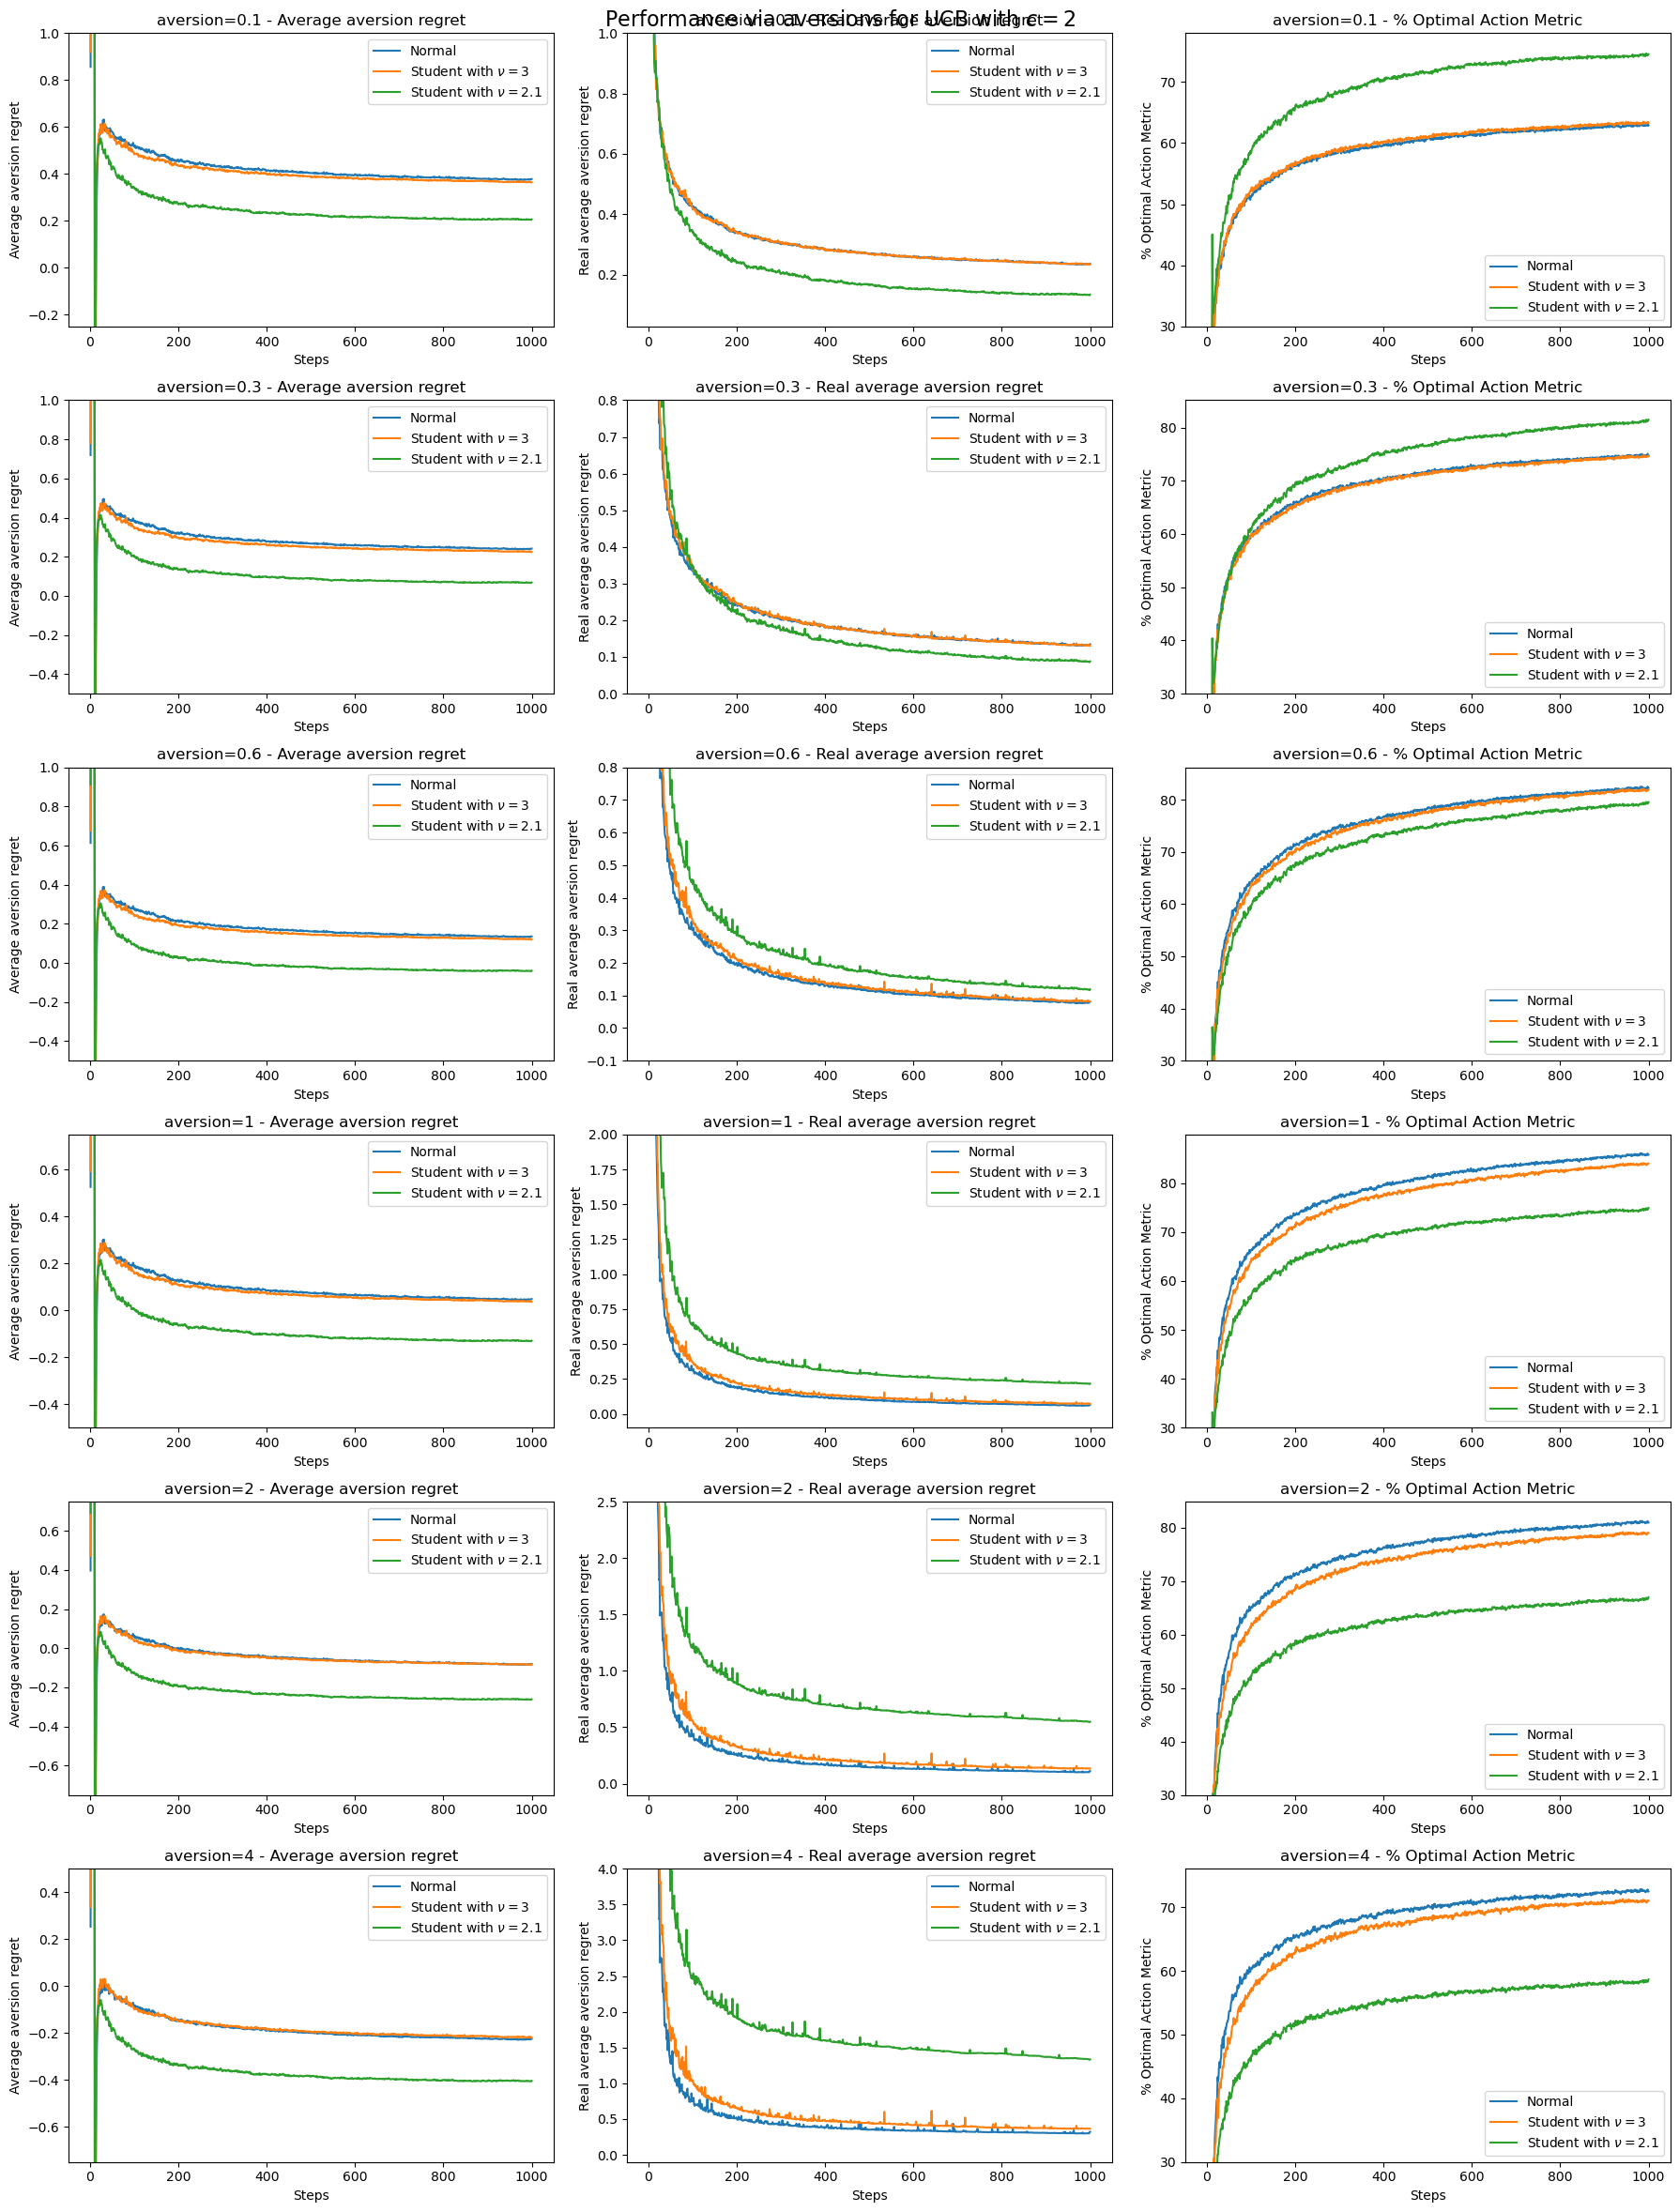
\includegraphics[scale=0.13,center]{images/theory_images/UCB/avers_avers.png}
    \end{frame}
    \begin{frame}{Результаты -- UCB}
        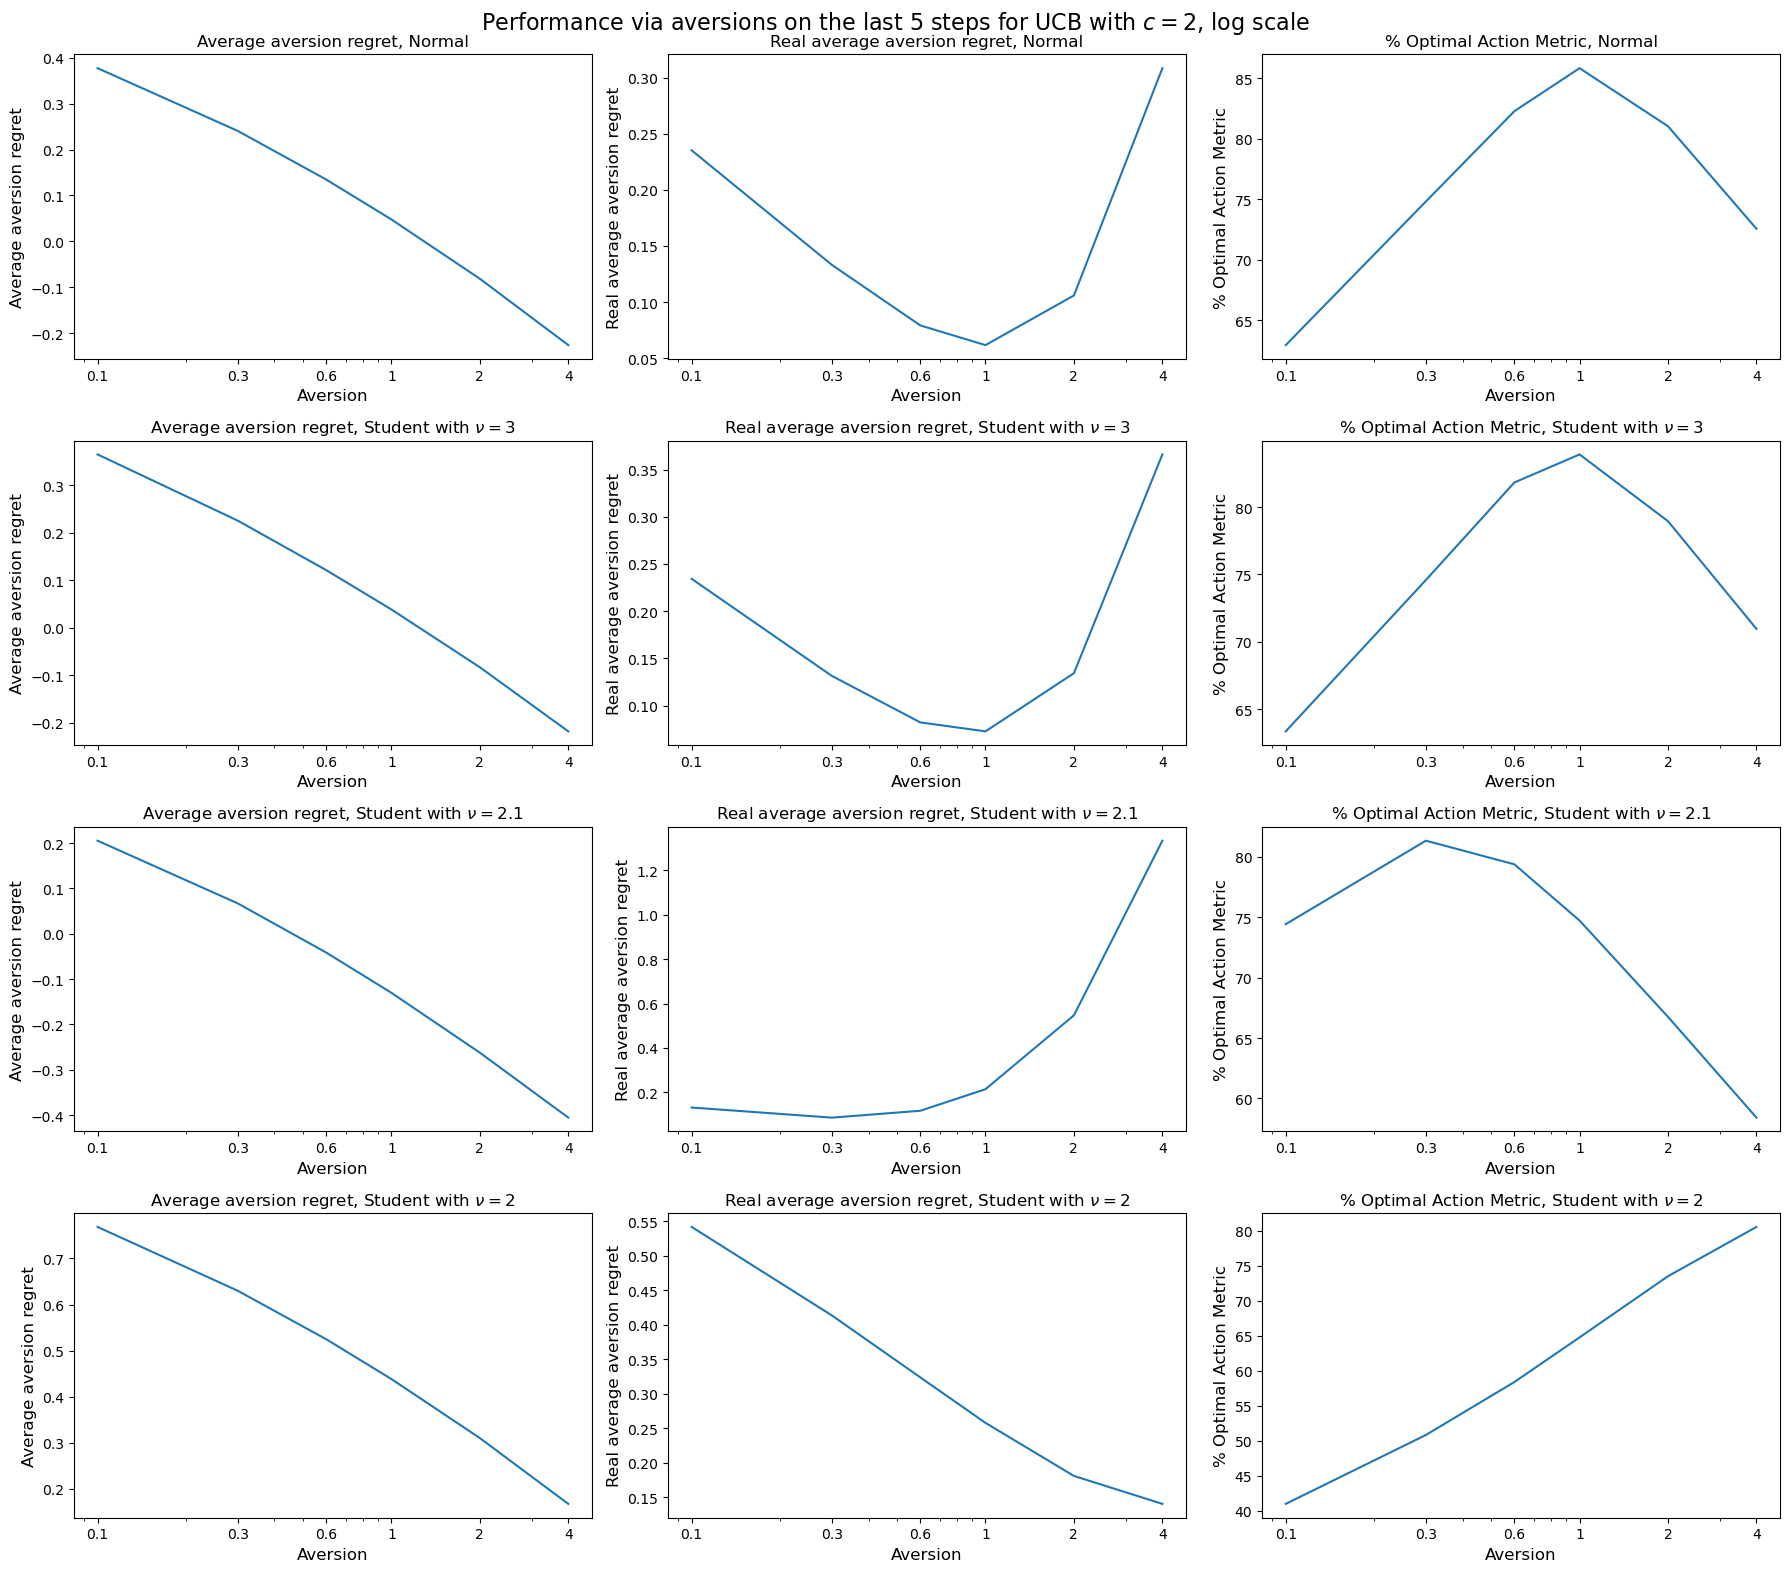
\includegraphics[scale=0.13,center]{images/theory_images/UCB/avers_last.png}
    \end{frame}
    \begin{frame}{Результаты -- gradient bandits}
        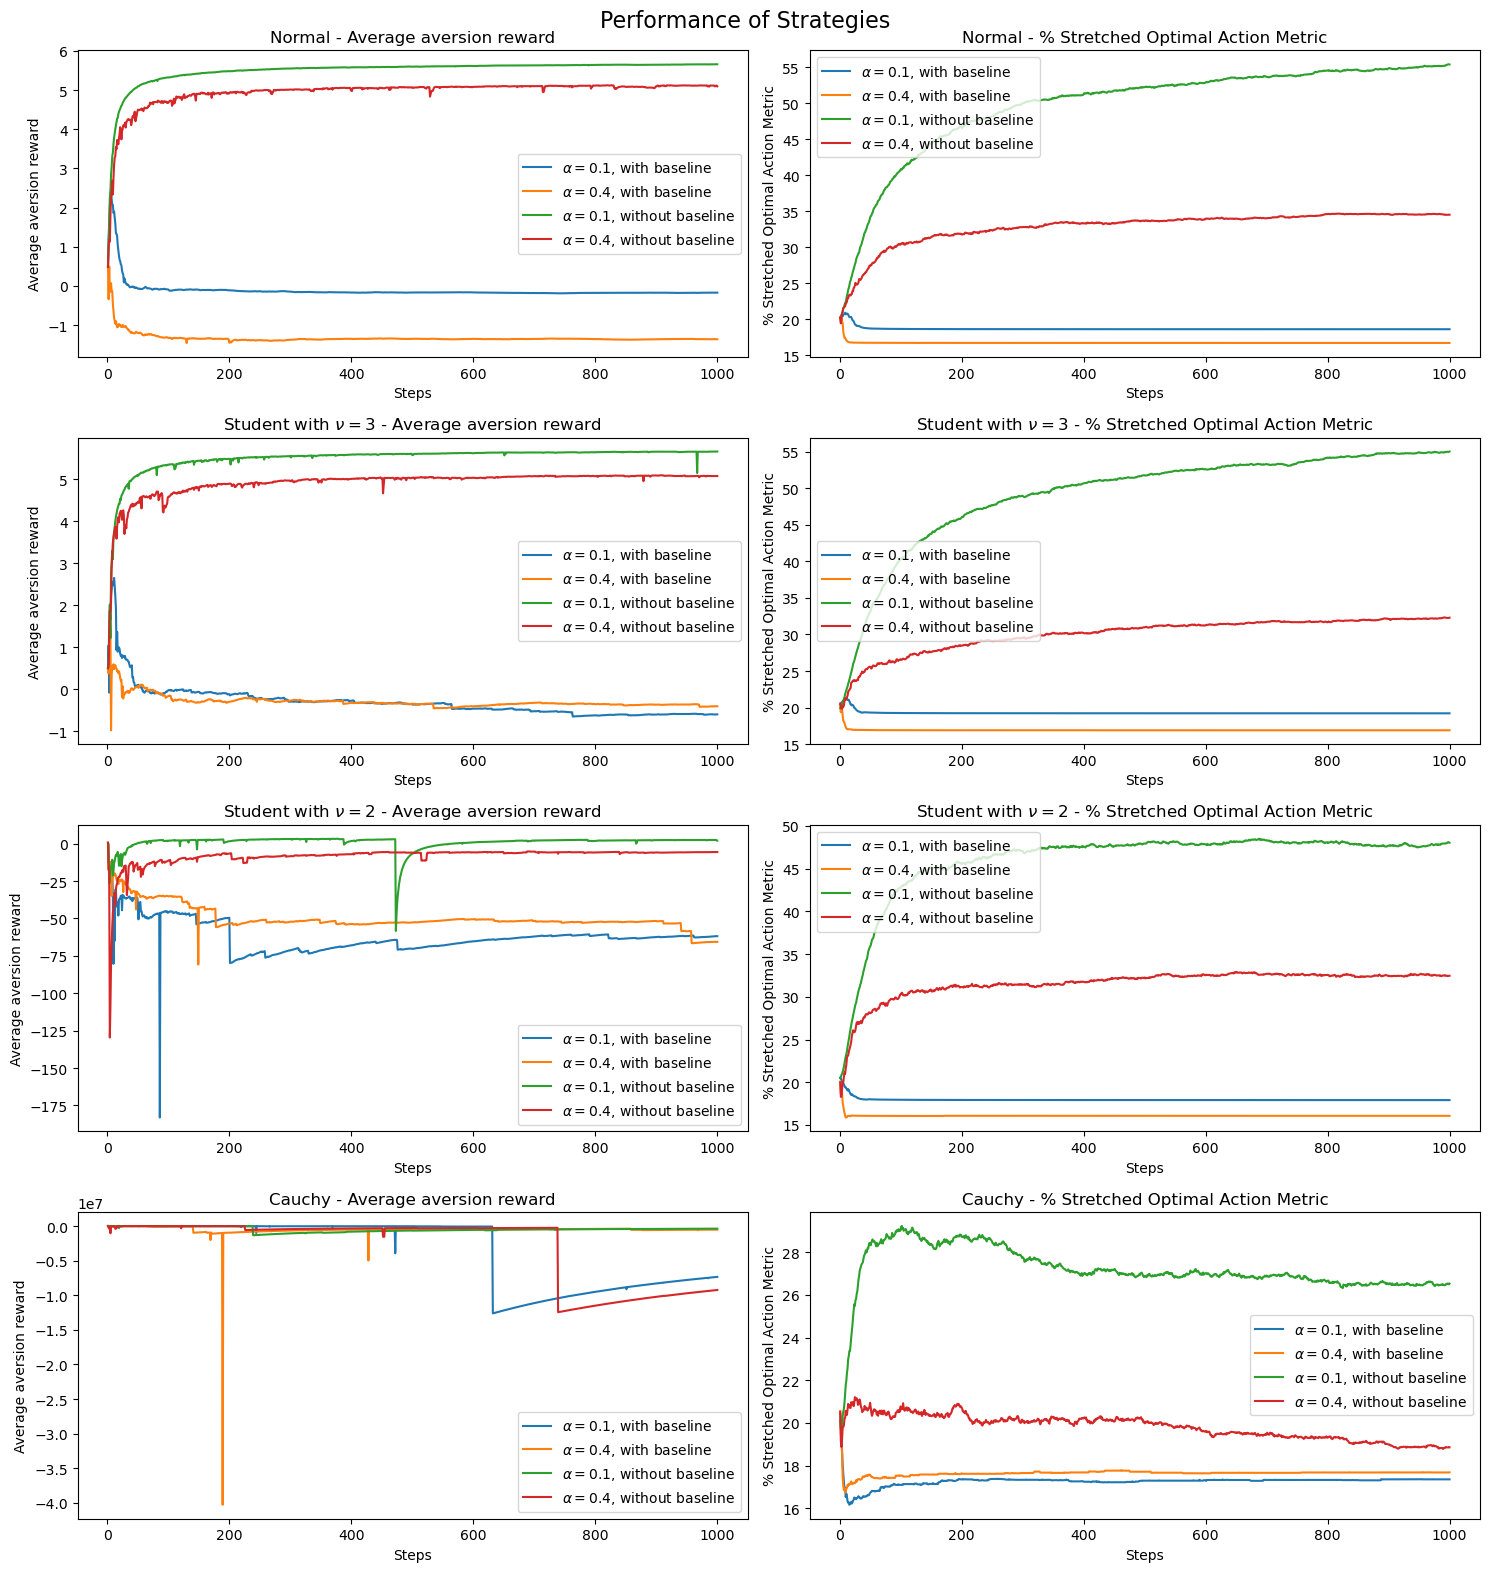
\includegraphics[scale=0.13,center]{images/theory_images/gradient_bandits/one_distr.png}
    \end{frame}
    \begin{frame}{Результаты -- gradient bandits}
        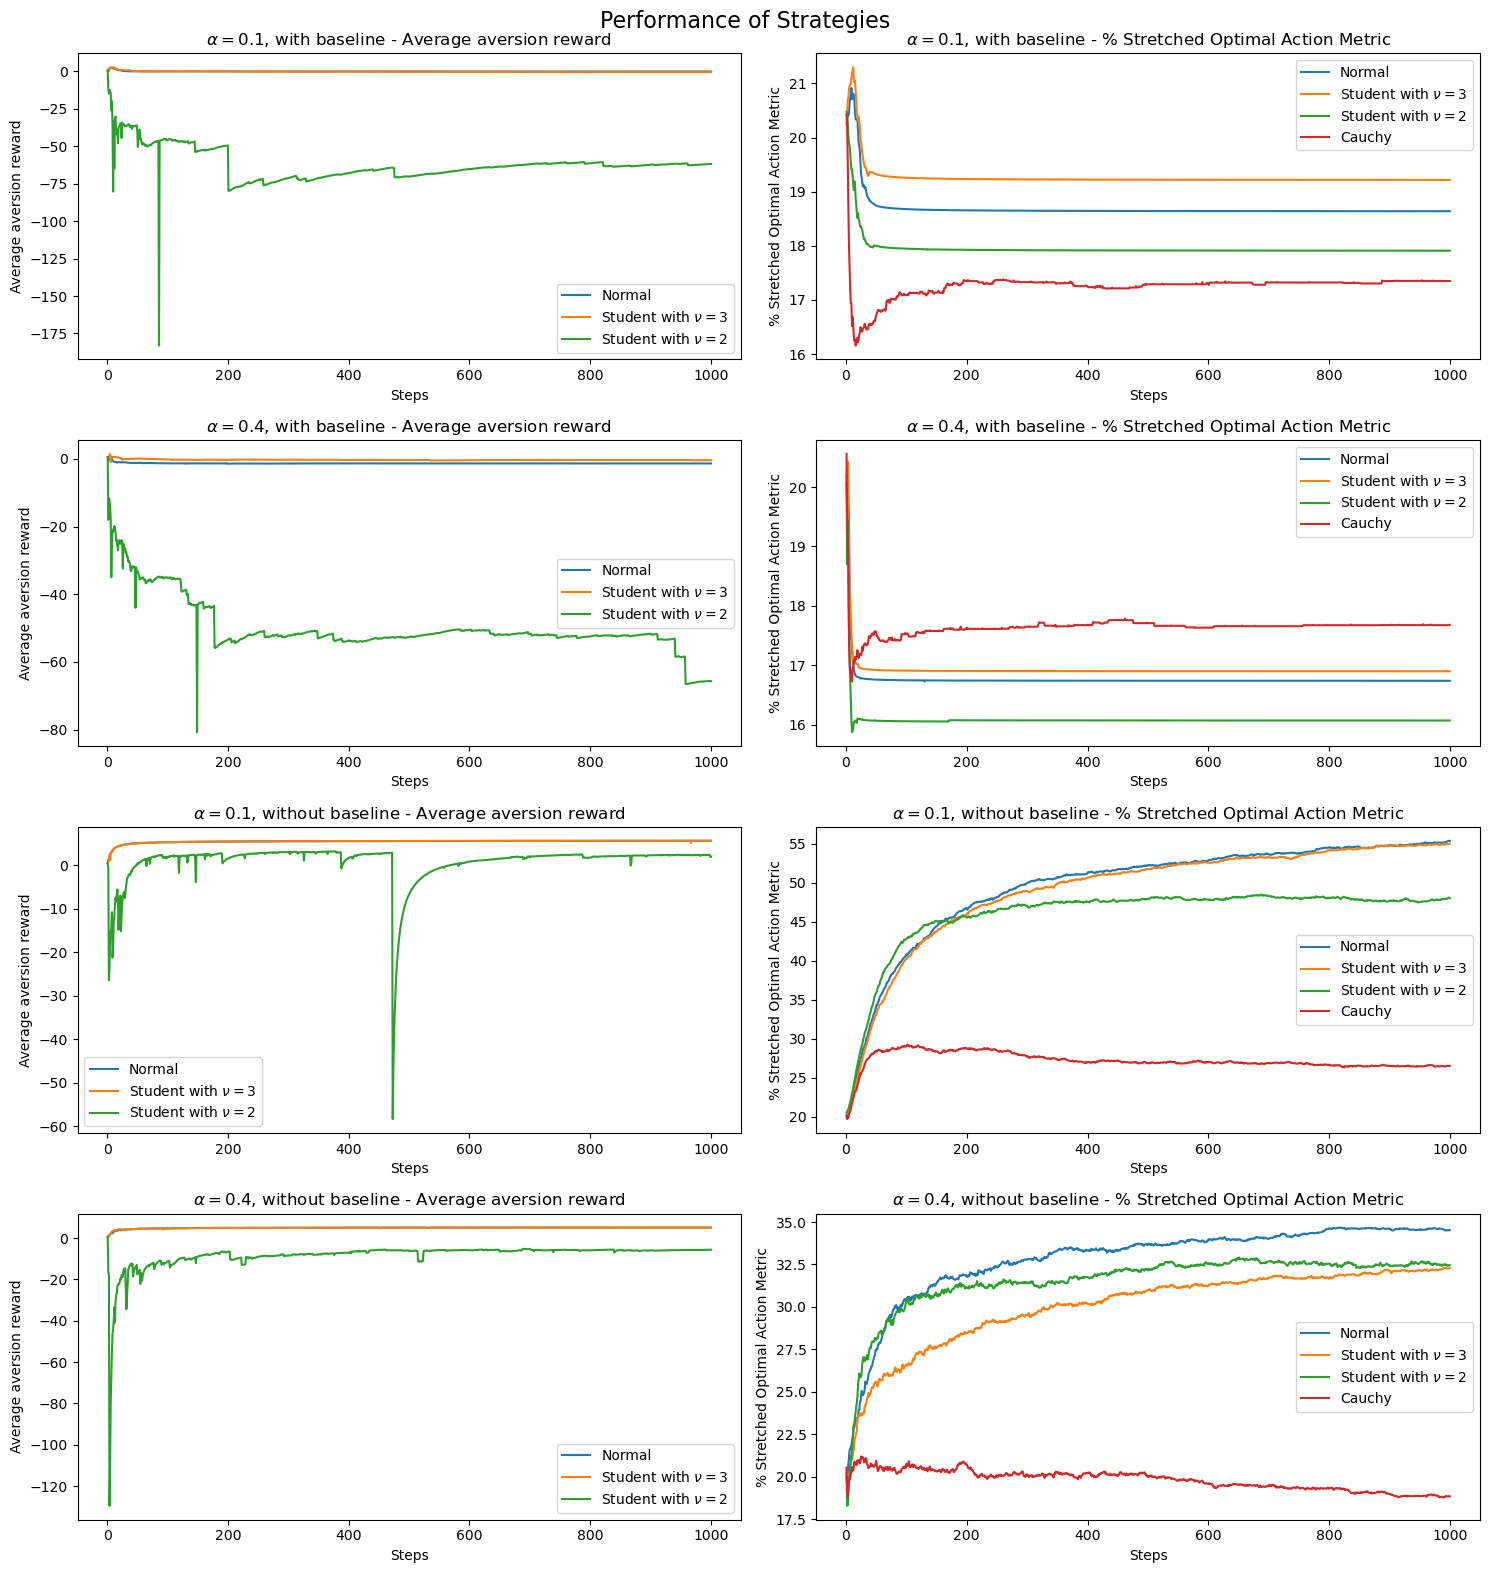
\includegraphics[scale=0.13,center]{images/theory_images/gradient_bandits/one_strat.png}
    \end{frame}
    \begin{frame}{Выводы}
        \begin{itemize}
            \item<1-> Алгоритм в сочетании с $\epsilon$-greedy дает отличное приближение вероятностей.
            \item<2-> При уменьшении $\nu$ VDBE и UCB начинают работать лучше, чем $\epsilon$-greedy.
            \item<3-> График зависимости точности оптимальных действий от коэффициента неприятия к риску имеет выраженный максимум.
        \end{itemize}
    \end{frame}

\section{Заключение}
    \begin{frame}{Заключение}
        В результате написания работы:
        \begin{itemize}
            \item<1-> Проанализированы известные подходы в классической задаче о многоруких бандитах на предмет применимости для распределений, отличных от нормального.
            \item<2-> Придуманы алгоритмы и подходы для решения задачи о многоруких бандитах с учетом степени отвращения к риску.
            \item<3-> Протестированы созданные подходы на различных распределениях, получены хорошие результаты.
        \end{itemize}
    \end{frame}

\section{Источники}
    \begin{frame}{Источники}
        \printbibliography
    \end{frame}

\end{document}
